\documentclass[11pt,a4paper,twoside]{report}

\usepackage[noTeX]{mmap}%чтобы можно было искать и копировать текст на русском и формулы
\usepackage[T2A]{fontenc}
\usepackage[utf8]{inputenc}
\usepackage[english,russian]{babel}
\usepackage{amssymb,amsfonts,amsmath,mathtext,enumerate,float,amsthm,xfrac,empheq} 
\usepackage{mathrsfs}%Ralph Smith’s Formal Script Font

\usepackage{setspace} 
\onehalfspacing

\usepackage{geometry}
\geometry{left=3cm, right=2cm, top=2cm, bottom=2.5cm}

\usepackage{tocloft}%чтобы точки были в содержании
\renewcommand{\cftsecleader}{\cftdotfill{\cftdotsep}}

\usepackage{tikz}%для рисования диаграмм
\tikzset{node distance=3cm, auto}

\usepackage{indentfirst}%чтобы первый параграф был с отступом

\usepackage{hyperref}%добавляет гиперссылки
\usepackage[hypcap]{caption}%чтобы правильно отрабатывался переход по ссылке на изображение
\usepackage{cancel}%для зачёркивания символов

\usepackage{biblatex}
\defbibheading{bibliography}{\chapter*{Литература}\addcontentsline{toc}{chapter}{Литература}}
\bibliography{main}
\AtEveryBibitem{\clearlist{language}}

%чтобы списки были более сжатыми по вертикали
\newlength{\wideitemsep}
\setlength{\wideitemsep}{.5\itemsep}
\addtolength{\wideitemsep}{-7pt}
\let\olditem\item
\renewcommand{\item}{\setlength{\itemsep}{\wideitemsep}\olditem}

\numberwithin{equation}{section}

\def\multiset#1#2{\ensuremath{\left(\kern-.3em\left(\genfrac{}{}{0pt}{}{#1}{#2}\right)\kern-.3em\right)}}

\newcommand{\coker}{\operatorname{coker}}
\newcommand{\im}{\operatorname{im}}
\newcommand{\tr}{\operatorname{tr}}
\renewcommand{\mod}{\operatorname{mod}\;}

\newcommand{\str}{\operatorname{Str}}
\newcommand{\symstr}{\operatorname{Sym-Str}}
\newcommand{\symd}{\operatorname{Sym-D}}
\newcommand{\supp}{\operatorname{supp}}

\newcommand{\rank}[1]{R\left(#1\right)}
\newcommand{\brank}[1]{\underline{R}\left(#1\right)}
\newcommand{\ceilfrac}[2]{\left\lceil \frac{#1}{#2} \right\rceil}
\newcommand{\ceil}[1]{\left\lceil #1 \right\rceil}

\newcommand{\ab}[1]{\left\langle #1 \right\rangle}
\newcommand{\mt}[1]{\ab{#1}}

\newcommand{\cb}[1]{\left\{ #1 \right\}}

\newcommand{\RR}{\mathbb{R}}
\newcommand{\ZZ}{\mathbb{Z}}
\newcommand{\QQ}{\mathbb{Q}}
\newcommand{\CC}{\mathbb{C}}

\newcommand{\GF}[1]{\mathbb{F}_{#1}}
\newcommand{\GL}[2]{GL_{#1}(#2)}

\newcommand{\fa}[1]{F_{#1}^{ab}}
\newcommand{\chr}[1]{\operatorname{char}(#1)}
\newcommand\restr[2]{{% we make the whole thing an ordinary symbol
  \left.\kern-\nulldelimiterspace % automatically resize the bar with \right
  #1 % the function
  \vphantom{\big|} % pretend it's a little taller at normal size
  \right|_{#2} % this is the delimiter
  }}
  
%чтобы у всех видов теорем нумерация была сквозной в пределах section
\newcounter{dummy} 

\newtheorem{theorem}[dummy]{Теорема}
\newtheorem{lemma}[dummy]{Лемма}
\newtheorem{prop}[dummy]{Утверждение}
\newtheorem{corollary}[dummy]{Следствие}
\newtheorem{conj}[dummy]{Гипотеза}
\newtheorem{remark}[dummy]{Замечание}
\theoremstyle{definition}
\newtheorem{definition}[dummy]{Определение}
\newtheorem{example}[dummy]{Пример}
\theoremstyle{remark}
\newtheorem{observation}[dummy]{Наблюдение}
\newtheorem{notation}[dummy]{Обозначение}
\newtheorem{reseach}[dummy]{Исследовательская задача}
\newtheorem{exercise}[dummy]{Упражнение}

\usepackage{mdframed}
\newmdtheoremenv{question}{Вопрос}

\begin{document}
	\begin{titlepage}
	\begin{center}
	
	\vspace{12em}
	
	\textbf{\Large Теоретико-групповой подход к быстрому умножению матриц}
	\vspace{1em}
	
	Иванов Дмитрий Михайлович - аспирант кафедры математической логики, алгебры\\
	и теории чисел Ярославского Государственного Университета

	\vspace{\fill}

	Ярославль 2013
	\end{center}
\end{titlepage}

	
	\tableofcontents 
	\clearpage
	
	\chapter*{Предисловие}
	\addcontentsline{toc}{chapter}{Предисловие}
	Данное учебное пособие предназначено для студентов, которые хотели бы больше узнать о современных алгоритмах для быстрого перемножения матриц и связанной с ними теорией. Для того, чтобы понять изложенный материал, будет достаточно начальных сведений из линейной алгебры и теории групп, всё, что будет сверх этого, уже содержится в пособии либо в основном тексте, либо в одном из подразделов \hyperref[appendix]{дополнения}.

Пособие представляет из себя по большей части перевод с пояснениями статей Кона, Уманса и других \cite{Cohn03,Cohn05,Cohn12}. Многие понятия введённые авторами не получили ещё устоявшегося перевода на русский, поэтому в таких случаях вслед за моим переводом будет дано их английское название. 

В начале пособия идёт перевод лекций Маркуса Блазера \cite{Lecture} о теории алгебраической сложности, без которой статьи Кона невозможно понять. 


		
	\chapter*{Список обозначений}
	\addcontentsline{toc}{chapter}{Список обозначений}
	\begin{tabular}{lp{11cm}}
  \textit{Обозначение} & \textit{Смысл} \\
  \hline
  $\ln x$ & натуральный лографм: $\log_e x$  \\
  $\left\lceil \frac{g}{f} \right\rceil$ & функция потолок, то есть округление $\frac{g}{f}$ до ближайшего целого в большую сторону (стр. \pageref{lem:bi:6.5})\\
  $\left\langle n,m,p \right\rangle_F$ & тензор прямоугольного матричного умножения для $n \times m$ и $m \times p$-матриц с элементами из поля $F$. Если $F = \mathbb{C}$, то будем писать просто $\left\langle n,m,p \right\rangle$ (стр. \pageref{matrix_tensor})\\
  $R(t)$ & ранг тензора $t$ (стр. \pageref{def:tensor_rank})\\
  $\omega$ & экспонента матричного умножения над полем $\mathbb{C}$ (стр. \pageref{def:omega})\\
  $Cyc_k$ & циклическая группа порядка $k$ со сложением в качестве групповой операции\\
  $[k]$ & множество $\left\{ 1,2, \dotsc, k \right\}$, где $k$ натуральное число \\
  $A \setminus B$ & множество ${\{a \in A \mid a \notin B\}}$\\
  $A - B$ & множество $\{a - b \mid a \in A, b \in B\}$, где $A$ и $B$ являются подмножествами абелевой группы\\
  $S_M$ & группа перестановок элементов множества $M$\\
  $S_n$ & группа перестановок элементов множества $[n]$\\
  $R[G]$ & групповая алгебра над $G$ с коэффициентами из $R$, где $G$ --- группа, а $R$ --- кольцо (стр. \pageref{group_algebra})\\
  $g \cdot a$ & элемент группы $G$ \textit{действует слева} на элемент множества $A$ (стр. \pageref{action})\\
  $a^g$ & элемент группы $G$ \textit{действует справа} на элемент множества $A$ (стр. \pageref{action})\\
  $H \rtimes G, \; G \ltimes H$ & полупрямое произведение (стр. \pageref{semidirect_product})\\
  $O(g(x))$ & $O$-большое от функции $g(x)$ (стр. \pageref{o_notation})\\
  $o(1)$ & функция, стремящаяся к 0 при стремлении к бесконечности какой-то переменной из контекста, например, таковой будет $1/x$ при $x \to \infty$ (стр. \pageref{little-oh})\\
  $\binom{N}{\mu}$ & мультиномиальный коэффициент, то есть $\frac{N!}{\mu_1! \dotsm \mu_n!}$ (стр. \pageref{lem:05:1.1})\\
  $2^S$ & множество всех подмножеств $S$ (стр. \pageref{def:05:6.5})\\
  $fin(S)$ & множества всех \textit{конечных} подмножеств $S$ (стр. \pageref{sec:general_model})\\
  $Q(S)$ & множество правых частных $S$, то есть $\{ s_1 s_2^{-1} \mid s_1, s_2 \in S\}$ (стр. \pageref{sec:realizing})\\
\end{tabular}

	
	\chapter*{Введение}
	\addcontentsline{toc}{chapter}{Введение}
	Задача умножения матриц является одной из самых фундаментальных проблем в алгоритмической линейной алгебре. Матричное умножение важно само по себе, но оно становится ещё важнее из-за множества задач, которые к нему сводятся.
 
В 1969 Штрассен \cite{Strassen:1969} создал \hyperref[Strassen_algorithm]{алгоритм} для умножения $n \times n$ матриц, который требовал $O(n^{2.81})$ операций. За этим открытием последовала серия улучшений, которые смогли дать лучшие оценки экспоненты матричного умножения. Копперсмит и Виноград \cite{Coppersmith:1990} в 1990 показали, что $\omega \leq 2.376$. Небольшим улучшением их метода стала работа Вильямс в 2011 \cite{Williams:2011}, которая показала, что $\omega \leq 2.3727$, что является наилучшей оценкой сверху на данный момент. 

Лучшей нижней оценкой является $2 \leq \omega$, её можно получить, если заметить, что для матричного произведения необходимо вычислить $n^2$ элементов. Многие исследователи верят, что эту нижнюю оценку можно достичь, то есть $\omega = 2$.

Недавно американские математики Кон и Уманс \cite{Cohn03} предложили новый теоретико-групповой подход для создания алгоритмов матричного умножения. В их схеме выбирается конечная группа $G$, удовлетворяющая определённому свойству, которое позволяет свести умножение $n \times n$ матриц к умножению элементов из \hyperref[group_algebra]{групповой алгебры} $\mathbb{C}[G]$. Это последнее умножение производится через преобразование Фурье, которое сводит его к нескольким меньшим матричным умножениям, чьи размеры зависят от \hyperref[def:characters_degree]{степеней характеров} $G$. Данное построение естественным образом даёт рекурсивный алгоритм, чьё время выполнения зависит от степеней характеров. Таким образом, проблема создания алгоритма матричного умножения в этой схеме переводится в область теории групп и \hyperref[representation]{теории представлений}.


	
	\chapter{Сложность билинейных задач}
	\section{Алгоритм Штрассена}\label{Strassen_algorithm}

\begin{definition}\cite{wiki:bf}
	Если $V$ --- это векторное пространство над полем скаляров $F$, то \textbf{билинейной формой} называют функцию $f: V \times V \to F$, которая удовлетворяет следующим условиям:
	\begin{enumerate}[(1)]
	     \item $f(u + v, w) = f(u, w) + f(v, w), f(u, v + w) = f(u, v) + f(u, w)$ и $f(kv, w) = kf(v, w) = f(v, kw)$ для всех $u, v, w \in V$ и всех $v, w \in V$.
	     \item $f$ называется \textbf{симметричной билинейной формой}, если она также удовлетворяет:
	     $f(v, w) = f(w, v)$ для всех $v, w \in V$
	\end{enumerate}
\end{definition}

Пусть даны две $n \times n$-матрицы $X=(x_{ik})$ и $Y=(y_{kj})$, чьи элементы являются неизвестными из поля $K$. Мы хотим вычислить их произведение $XY=(z_{ij})$. Элементы $z_{ij}$ задаются следующими хорошо известными билинейными формами:
\[
	z_{ij}= \sum\limits_{k=1}^{n} x_{ik} y_{kj}, \; 1 \leq i,j \leq n.
\]

Каждый $z_{ij}$ --- это сумма $n$ произведений, поэтому чтобы вычислить $z_{ij}$ нужно $n$ умножений и $n-1$ сложение. В итоге получим алгоритм, требующий в общей сложности $n^3$ умножений и $n^2(n-1)$ сложение. Этот алгоритм выглядит так естественно и интуитивно, что очень сложно представить, что существует лучший способ перемножения матриц. Однако в 1969 году Штрассен \cite{Strassen:1969} придумал как перемножить $2 \times 2$-матрицы всего за 7 умножений, но 18 сложений.

Пусть $z_{ij}\; 1 \leq i,j \leq 2$ задаются как
\[
	\left( 
	\begin{array}{cc}
	  z_{11} & z_{12}\\
	  z_{21} & z_{22}
	\end{array}
	 \right)=
	 \left( 
	\begin{array}{cc}
	  x_{11} & x_{12}\\
	  x_{21} & x_{22}
	\end{array}
	 \right)
	 \left( 
	\begin{array}{cc}
	  y_{11} & y_{12}\\
	  y_{21} & y_{22}
	\end{array}
	 \right).
\]
Вычислим семь произведений
\[
	\begin{array}{l}
	  p_1=(x_{11}+x_{22})(y_{11}+y_{22})\\
  	  p_2=(x_{11}+x_{22})y_{11}\\
  	  p_3=x_{11}(y_{12}-y_{22})\\
  	  p_4=x_{22}(-y_{11}+y_{12})\\
  	  p_5=(x_{11}+x_{12})y_{22}\\
  	  p_6=(-x_{11}+x_{21})(y_{11}+y_{12})\\
  	  p_7=(x_{12}-x_{22})(y_{21}+y_{22})\\
	\end{array}
\]
и тогда можно выразить каждый из $z_{ij}$ как линейную комбинацию этих семи произведений, а именно
\[
	\left( 
	\begin{array}{cc}
	  z_{11} & z_{12}\\
	  z_{21} & z_{22}
	\end{array}
	 \right)=
	 \left( 
	\begin{array}{cc}
	  p_1+p_4-p_5+p_7 & p_3+p_5\\
	  p_2+p_4 & p_1+p_3-p_2+p_6
	\end{array}
	 \right).
\]

Возникает вопрос, стоит ли сохранять одно умножение, чтобы получить 14 дополнительных сложений? Важным моментом является то, что алгоритм Штрассена работает не только над полями, но и над некоммутативными кольцами. В частности, элементы $2 \times 2$-матриц могут сами быть матрицами, и можно применять этот алгоритм рекурсивно. А для матриц умножение --- по крайней мере если использовать наивный алгоритм --- гораздо дороже сложения, а именно \hyperref[o_notation]{$O(n^3)$} против $n^2$.











	\section{Общая модель вычислений и сложности}\label{sec:general_model}

В этом разделе будет определена структура вычислений и стоимости достаточно общая, чтобы объяснить все последующие примеры. Для множества $S$ обозначим через $fin(S)$ множества всех конечных подмножеств $S$.

\begin{definition}
  \textbf{Вычислительная структура} --- это множества $M$ вместе с отображением $\gamma:M \times fin(M) \to [0, \infty]$ таким, что:
  \begin{enumerate}[1.]
    \item $im(\gamma)$ хорошо упорядочено, то есть любое подмножество $im(\gamma)$ имеет минимум.
    \item $\gamma(\omega,U)=0$, если $\omega \in U$
    \item $U \subseteq V \Longrightarrow \gamma(\omega,V) \leq \gamma(\omega,U) $ для всех $\omega \in M; \; U,V \subseteq fin(M)$
  \end{enumerate}
\end{definition}

$M$ --- множество объектов, с которыми мы производим вычисления. $\gamma(\omega,U)$ --- стоимость вычисления $\omega$ при данном $U$ <<за один шаг>>. \\
$\gamma(\omega,U)=0$, если $\omega \in U$ потому, что не нужно платить за уже вычисленный элемент. $\gamma(\omega,U)=1$, если существуют $u,v \in U$ такие, что $\omega = u\; op\; v$, где $op$ обозначает какую-то арифметическую операцию, то есть $\omega$ вычисляется из $u$ и $v$ за одну арифметическую операцию. Во всех остальных случаях $\gamma(\omega,U)=\infty$, то есть нельзя вычислить $\omega$ <<за один шаг>> из $U$.

\begin{definition}
  \begin{enumerate}[1.]
	\item  Последовательность $\beta=(\omega_1, \ldots, \omega_m)$ элементов из $M$ называется \textbf{вычислением} или \textbf{алгоритмом} со входом $X \subseteq fin(M)$, если
    	\[
    		\forall j \leq m: \omega_j \in X \lor \gamma(\omega_j, V_j) < \infty \mbox{, где } V_j = \{ \omega_1, \ldots, \omega_{j-1} \}
    	\]
    	\item $\beta$ \textbf{вычисляет} множество $Y \in fin(M)$, если $Y \subseteq \{ \omega_1, \ldots, \omega_m \}$
    	\item \textbf{Стоимость} $\beta$ --- это $\Gamma(\beta, X) \overset{Def}{=} \sum\limits_{j=1}^{m} \gamma(\omega,V_j)$  
  \end{enumerate}
\end{definition}
В вычислении каждый $\omega_i$ может быть получен из вычисленных до этого элементов, то есть элементов $V_j$ или из $X$ (<<входа>>).

\begin{definition}
  \textbf{Сложность} $Y$ при данном $X$ определяется как
  \[
  	C(Y,X) \overset{Def}{=} min \{ \Gamma(\beta,X) \mid \beta \mbox{ вычисляет } Y \mbox{ по } X \}
  \]
\end{definition}
Сложность множества $Y$ --- это не более чем стоимость самого дешевого вычисления, с помощью которого можно получить $Y$. 

Если множество $X$ пустое или понятно из контекста, то вместо $C(Y,X)$ будем писать $C(Y)$. Если вычисляется один элемент, то есть $Y = \left\{ y \right\}$, то вместо $C(\left\{ y \right\},X)$ будет $C(y,X)$.

\textbf{Мерой Островского} называют вычислительную структуру, где $M = K(x_1, \ldots , x_n)$ --- поле рациональных функций от неизвестных $x_1, \ldots , x_n$ над полем $K$, и где есть четыре (или три) бинарных операции, а именно умножение, деление, сложение и вычитание. Деление --- частичная операция, определённая только если второй аргумент ненулевой. Для любого $\lambda \in K$ существует ещё унарная операция, а именно умножение на скаляр $\lambda$. Стоимости этих операций задаются так:
\begin{center}
  \begin{tabular}{c|c}
	  операция  & стоимость   \\
	  \hline
	  $\cdot,/$ & 1 \\
	  $+,-$ & 0 \\
	  $\lambda \cdot$ & 0
  \end{tabular}
\end{center}

Сложность, даваемая мерой Островского, будет обозначаться как $C^{*/}$, а если не используется деление, то $C^{*}$.



	\section{Билинейные задачи}

\begin{definition}\cite{wiki:qf}
  \textbf{Квадратичной формой} называют однородный многочлен степени 2 от нескольких переменных. Например,
  \[
  	4x^2+2xy-3y^2
  \]
  будет квадратичной формой от переменных $x$ и $y$.
\end{definition}

Пусть $K$ --- поле, обычно оно называется полем скаляров, и пусть $M=K(x_1, \ldots, x_N)$. Мера Островского потребуется для следующего. Мы будем задаваться вопросами вида
\[
	C^{*/}(F)=?,
\]
где $F=\{ f_1, \ldots, f_k \}$ --- множество квадратичных форм
\[
	f_\kappa = \sum\limits_{\mu,\nu=1}^{N} t_{\kappa \mu \nu} x_\mu x_\nu.
\]

Большую часть времени мы будем рассматривать особый случай билинейных форм, то есть наши переменные разделены на два непересекающихся множества и только произведения одной переменной из первого множества и одной из второго встречаются в $f_k$.

<<Трехмерный массив>> $t:=(t_{\kappa \mu \nu})_{\kappa = 1, \ldots, k;  \mu ,\nu = 1, \ldots, N } \in K^{k \times N \times N}$ называется \textbf{тензором, соответствующим $F$}. Так как $x_\mu x_\nu = x_\nu x_\mu$, существует несколько тензоров, представляющих одну и ту же задачу $F$. Тензор $s$ является \textbf{симметрически эквивалентным} тензору $t$, если
\[
	s_{\kappa \mu \nu} + s_{\kappa \nu \mu} = t_{\kappa \mu \nu} + t_{\kappa \nu \mu} \mbox{ для всех } \kappa, \mu, \nu.
\]

Два тензора описывают одно и тоже множество квадратичных форм, если они симметрически эквивалентны.



	\section{Ранг билинейных задач}

Штрассен \cite{Strassen:1973} показал, что для вычисления множества билинейных форм деления не нужны при условии, что поле скаляров достаточно большое.

\begin{theorem}\label{th:3.1}
Пусть $f_\kappa = \sum\limits_{\mu,\nu=1}^{N} t_{\kappa \mu \nu} x_\mu x_\nu, \; 1 \leq \kappa \leq k$. Если $|K| = \infty$ и $C^{*/}(F)=\ell$, тогда существует оптимальное вычисление (то есть за меньшее количество операций задачу не посчитать), состоящее из произведений
\[
	P_\lambda = \left( \sum\limits_{i=1}^{N} u_{\lambda i} x_i  \right) \left( \sum\limits_{i=1}^{N} v_{\lambda i} x_i  \right), \; 1 \leq \lambda \leq \ell,
\]  
такое, что $F \subseteq lin_K \{ P_1 , \ldots, P_\ell  \} = \{ \alpha_1 P_1 + \ldots + \alpha_\ell P_\ell |\alpha_i \in K \}$. В частности, $C^{*/}(F)=C^{*}(F)$.
\end{theorem}

Матричное умножение и умножение многочленов являются билинейными задачами, поэтому мы можем разделить переменные на два множества $\{ x_1, \ldots, x_M  \}$ и $\{ y_1, \ldots, y_N  \}$ и записать квадратичные формы как 
\[
	f_k = \sum\limits_{\mu=1}^{M} \sum\limits_{\nu=1}^{N} t_{\kappa \mu \nu} x_\mu y_\nu, \; 1 \leq \kappa \leq k.
\]
Тензор $(t_{\kappa \mu \nu}) \in K^{k \times M \times N}$ будет единственным и поэтому понятие симметрической эквивалентности не потребуется.

Теорема \ref{th:3.1} говорит нам, что при использовании меры Островского мы должны рассматривать только произведения линейных форм. При вычислении билинейных форм будет естественным ограничиться произведениями вида, где линейная форма от переменных $\{ x_1, \ldots, x_M  \}$  умножается на линейную форму от $\{ y_1, \ldots, y_N  \}$.

\begin{definition}
  Минимальное число произведений
  \[
  	P_\lambda = \left( \sum\limits_{\mu=1}^{M} u_{\lambda \mu} x_\mu \right) \left( \sum\limits_{\nu=1}^{N} v_{\lambda \nu} y_\nu \right),\; 1 \leq \lambda \leq l
  \]
  таких, что $F \subseteq lin_K \{ P_1 , \ldots, P_\ell  \}$ называется \textbf{рангом} $F = \{ f_1, \ldots f_k \}$ или \textbf{билинейной сложностью $F$} и обозначается как $R(F)$.
\end{definition}

Мы можем также определить ранг в терминах тензоров. Пусть $(t_{\kappa \mu \nu})$ тензор задачи $F$. Имеем, что $ R(F) \leq l$\\
$\Longleftrightarrow $ существуют линейные формы  $u_1, \ldots, u_\ell $ от $x_1, \ldots, x_M$  и $v_1, \ldots, v_\ell $  от $y_1, \ldots, y_N$  такие, что $F  \subseteq lin_K \{ u_1v_1 , \ldots, u_\ell v_\ell  \}$\\
$\Longleftrightarrow$ существуют $w_{\lambda \kappa} \in K,\; 1 \leq \lambda \leq l, \; 1 \leq \kappa \leq k$  такие, что 
\[
	f_\kappa = \sum\limits_{\lambda=1}^{l} w_{\lambda \kappa} u_\lambda v_\lambda = \sum\limits_{\lambda=1}^{l} \left( \sum\limits_{\mu=1}^{M} u_{\lambda \mu} x_\mu \right)\left( \sum\limits_{\nu=1}^{N} v_{\lambda \nu}y_\nu \right), \; 1 \leq \kappa \leq k.
\]
Сравнив коэффициенты, получим
\[
	t_{\kappa \mu \nu} = \sum\limits_{\lambda=1}^{l} w_{\lambda \kappa} u_{\lambda \mu} v_{\lambda \nu}, \; 1 \leq \kappa \leq k, \; 1 \leq \mu \leq M, \; 1 \leq \nu \leq N.
\]

\begin{definition}
  Пусть $w \in K^k,\; u \in K^M,\; v \in K^N$. Тензор $w \otimes u \otimes v \in K^{k \times M \times N}$ с элементом $w_k u_\mu v_\nu$ в позиции $(\kappa, \mu, \nu)$ называется \textbf{триадой}. 
\end{definition}

Из приведённых выше вычислений получим, что $R(F) \leq l$\\
$\Longleftrightarrow $ существуют $w_1, \ldots, w_\ell \in K^k, \; u_1, \ldots, u_\ell \in K^M$ и $v_1, \ldots, v_\ell \in K^N $ такие, что
\[
	t = (t_{\kappa \mu \nu}) = \sum\limits_{\lambda=1}^{l} \underbrace{w_\lambda \otimes u_\lambda \otimes v_\lambda}_\text{триада}.
\]

Определим \phantomsection \label{def:tensor_rank} ранг $R(t)$ тензора $t$ как минимальное число триад таких, что $t$ является их суммой. Каждое множество билинейных форм $F$  имеет соответствующий тензор $t$ и наоборот. Как видно их ранги совпадают.

Мультипликативная сложность и ранг линейно связаны.
\begin{theorem}\label{th:bi:3.7} 
  Пусть $F = \left\{ f_1, \dotsc, f_k \right\}$ --- это множество билинейных форм от переменных $\left\{ x_1, \dotsc, x_M \right\}$ и $\left\{ y_1, \dotsc, y_N \right\}$. Тогда
\[
	C^{*/}(F) \leq R(F) \leq 2 C^{*/}(F).
\]
\end{theorem}
\begin{proof}
  Первое неравенство должно быть ясно --- число билинейных умножений никак не может быть меньше числа обычных умножений. Для второго неравенства предположим, что $C^{*/}(F) = \ell$ и рассмотрим оптимальное вычисление. Мы имеем
\begin{align*}
  f_\kappa & = 
\sum_{\lambda=1}^{\ell} w_{\lambda \kappa} 
\left( \sum_{\mu=1}^{M} u_{\lambda \mu} x_{\mu} + \sum_{\nu=1}^{N} u_{\lambda \nu}' y_{\nu} \right)
\left( \sum_{\mu=1}^{M} v_{\lambda \mu}' x_{\mu} + \sum_{\nu=1}^{N} v_{\lambda \nu} y_{\nu} \right)\\
  & = 
\sum_{\lambda=1}^{\ell} w_{\lambda \kappa} \left( \sum_{\mu=1}^{M} u_{\lambda \mu} x_{\mu} \right) \left( \sum_{\nu=1}^{N} v_{\lambda \nu} y_{\nu} \right) + 
\sum_{\lambda=1}^{\ell} w_{\lambda \kappa} \left( \sum_{\mu=1}^{M} v_{\lambda \mu}' x_{\mu} \right)\left( \sum_{\nu=1}^{N} u_{\lambda \nu}' y_{\nu} \right).
\end{align*}
Члены вида $x_i x_j$ и $y_i y_j$ должны компенсировать друг друга, так как они не появляются в $f_{\kappa}$.
\end{proof}





	\section{Экспонента матричного умножения}

Обозначим через $M_K(n)$ общее число арифметических операций $\left\{ \times , +, - \right\}$ необходимых чтобы перемножить две $n \times n$-матрицы над полем $K$.
\begin{definition}\label{def:omega}
	\textbf{Экспонентой матричного умножения над $K$} называют наименьшее действительное число $\omega(K) > 0$, определяемое как
	\[
		\omega(K) := \inf \left\{ \tau \in \mathbb{R}^+ \mid M_K(n) = O(n^\tau), n \to \infty \right\}
	\]
\end{definition}
Обозначение $\omega(K)$ призвано показать возможную зависимость от базового поля $K$. Было доказано, что $\omega(K)$ не измениться, если мы заменим $K$ на любое алгебраическое расширение $\overline{K}$ \cite[383]{bur}. Также было доказано, что $\omega(K)$ определяется только характеристикой $Char(K)$ поля $K$, поэтому $\omega(K) = \omega(\mathbb{Q})$, если $Char(K) = 0$, и $\omega(K) = \omega(\mathbb{Z}_p)$ в противном случае, где $\mathbb{Z}_p$ --- это конечное поле целых чисел по модулю простого $p$ с характеристикой $p$ \cite{Pan1984}. Так как $Char(\mathbb{C}) = Char(\mathbb{R}) = Char(\mathbb{Q}) = 0$, это означает, что $\omega(\mathbb{C}) = \omega(\mathbb{R}) = \omega(\mathbb{Q})$. В этом подразделе мы продолжим писать $\omega(K)$, чтобы показать зависимость от базового поля, но в следующих разделах оставим формализм и будем писать просто $\omega$, потому как дальше речь пойдёт исключительно о произведениях комплексных матриц.

Но вернёмся к $M_K(n)$. Чтобы получить произведение $n \times n$-матриц $A B = C$ при помощи стандартного алгоритма, потребуется вычислить $n^2$ элементов вида $C_{ik} = \sum_{1 \leq j \leq n} A_{ij} B_{jk}$ для всех $1 \leq i,k \leq n$. Это потребует $n^3$ умножений и $n^3 - n^2$ сложений, что даёт верхнюю оценку $M_K(n) = 2n^3 - n^2 < 2 n^3 = O(n^3)$, то есть $M_K(n) < C' n^3$ для константы $C' = 2$, и означает верхнюю оценку $\omega(K) \leq 3$. Для нижней оценки заметим, что так как произведение двух $n \times n$-матриц состоит из $n^2$ элементов, то общее число операций будет по меньшей мере равнo $C n^2$ для $C \geq 1$, что обозначается как $M_K(n) = \Omega(n^2)$ и эквивалентно нижней оценке $2 \leq \omega(K)$ \cite[375]{bur}. Неформально мы доказали следующий элементарный результат:

\begin{prop}\label{prop:mol:2.11}
     Для любого поля $K$
	\begin{enumerate}
	     \item $2 \leq \omega(K) \leq 3$
	     \item $\omega(K) = h \iff \Omega(n^{h + \varepsilon}) = M_K(n) = O(n^{h + \varepsilon})$, где $h$ минимально для любого $\varepsilon > 0$
	\end{enumerate}
\end{prop}

Следующее утверждение связывает экспоненту и концепцию билинейного ранга:
\begin{prop}\label{prop:bur:15.1}(утверждение 15.1 из \cite[376-377]{bur})
Для любого поля $K$
	\[
		\omega(K) = \inf \{ \tau \in \mathbb{R} \mid R(\langle n,n,n \rangle) = O(n^\tau), n \to \infty \},
	\]
	где $\langle n,n,n \rangle$ обозначает тензор матричного умножения двух $n \times n$-матриц над полем $K$.  
\end{prop}
Это означает, что для данного поля $K$ и любого $\varepsilon > 0$ существует константа $C_{K, \varepsilon}$, независящая от $n$ такая, что $R(\left\langle n,n,n \right\rangle) \leq C_{K,\varepsilon} n^{\omega(K)+\varepsilon}$ для всех $n$. Есть гипотеза, что $\omega(\mathbb{C}) = 2$. С этого момента $\omega$ будет обозначать $\omega(\mathbb{C})$.


	\section{Тензоры}

В этом разделе будут введены некоторые операции над тензорами и изучено то, как они влияют на ранг.

Далее $\langle k,m,n \rangle:K^{k \times m} \times K^{m \times n} \to K^{k \times n}$ обозначает билинейное отображение, которое переводит $k \times m$-матрицу $A$ и $m \times n$-матрицу $B$ в их произведение $AB$. Потому как нет опасности запутаться, также будет обозначаться соответствующий тензор и множество билинейных форм
\[
	\left\{ \sum\limits_{\mu=1}^{m} X_{\kappa \mu} Y_{\mu \nu}| 1 \leq \kappa \leq k,\; 1 \leq \nu \leq n \right\}.
\]

\subsection{Перестановки}

Пусть $t \in K^{k \times m \times n}$ и $t = \sum_{j=1}^{r} t_j$ с триадами $t_j = a_{j1} \otimes a_{j2} \otimes a_{j3}, \; 1 \leq j \leq r $. Пусть $\pi \in S_3$. Для триады $t_j$ пусть $\pi t_j = a_{j \pi^{-1}(1)} \otimes a_{j \pi^{-1}(2)} \otimes a_{j \pi^{-1}(3)}$ и $\pi t = \sum_{j=1}^{r} \pi t_j$. Заданное таким образом отображение $\pi$ будет вполне определено, то есть не будет зависеть от способа декомпозиции $t$ в сумму триад. Чтобы это увидеть, пусть $t = \sum_{i=1}^{s} b_{i1} \otimes b_{i2} \otimes b_{i3}$ --- вторая декомпозиция $t$. Знаем, что
\[
	\sum_{j=1}^{r} a_{j1} \otimes a_{j2} \otimes a_{j3} = \sum_{i=1}^{s} b_{i1} \otimes b_{i2} \otimes b_{i3}.
\]
И хотим доказать, что
\[
	\sum_{j=1}^{r} a_{j \pi^{-1}(1)} \otimes a_{j \pi^{-1}(2)} \otimes a_{j \pi^{-1}(3)} = \sum_{i=1}^{s} b_{i \pi^{-1}(1)} \otimes b_{i \pi^{-1}(2)} \otimes b_{i \pi^{-1}(3)}.
\]
Пусть $a_{j1} = \left( a_{j11}, \dotsc, a_{j1k} \right)$ и $b_{i1} = \left( b_{i11}, \dotsc, b_{i1k} \right)$, и пусть $a_{j2}, \; a_{j3}, \; b_{j2}, \; b_{j3}$ задаются аналогично.
Получится, что у тензора $t$ в позиции $\left( e_1,e_2,e_3 \right)$ стоит
\[
	t_{e_1e_2e_3} = \sum\limits_{j=1}^{r} a_{j1e_1} \otimes a_{j2e_2} \otimes a_{j3e_3} = \sum\limits_{i=1}^{s} b_{i1e_1} \otimes b_{i2e_2} \otimes b_{i3e_3}.
\]
Таким образом, у тензора $\pi t$ в позиции $(e_1, e_2, e_3)$ стоит
\[
	\begin{array}{rcl}
	  \pi t_{e_1e_2e_3} & = & \sum\limits_{j=1}^{r} a_{j \pi^{-1}(1) e_{\pi^{-1}(1)}} \otimes a_{j \pi^{-1}(2) e_{\pi^{-1}(2)}} \otimes a_{j \pi^{-1}(3) e_{\pi^{-1}(3)}}\\
	  & = & \sum\limits_{i=1}^{s} b_{i \pi^{-1}(1) e_{\pi^{-1}(1)}} \otimes b_{i \pi^{-1}(2) e_{\pi^{-1}(2)}} \otimes b_{i \pi^{-1}(3) e_{\pi^{-1}(3)}}.
	\end{array}
\]
\begin{question}
  Не совсем понятно, как приведённое равенство доказывает утверждение о том, что действие вполне определено. 
\end{question}

\begin{figure}[H]
	\centering
    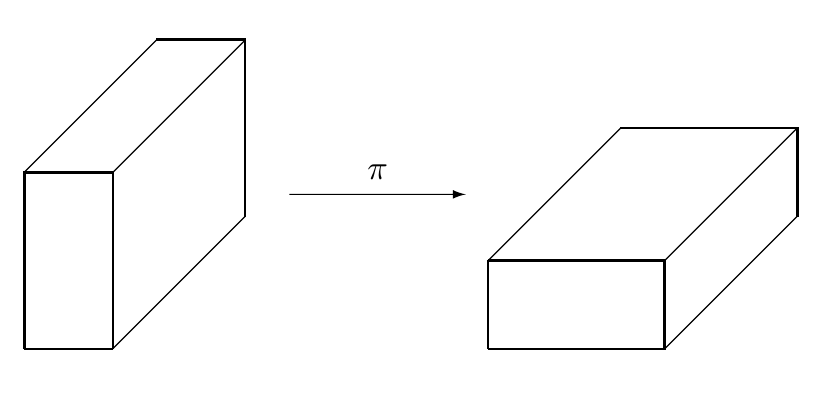
\includegraphics[width=0.5\textwidth]{figures/dimensions_permutation}
	\caption{Перестановка измерений}
	\label{fig:dimensions_permutation}
\end{figure}

Доказательство следующей леммы очевидно.
\begin{lemma}\label{lem:bi:4.3}
  $R(t) = R(\pi t)$
\end{lemma}

Кроме перестановки измерений тензора можно также переставлять его слои. Пусть $t=(t_{ij \ell}) \in K^{k \times m \times n}$ и $\sigma \in S_k$. Тогда для $t'=(t_{\sigma(i)j \ell})$, $R(t')=R(t)$.
\begin{figure}[H]
	\centering
    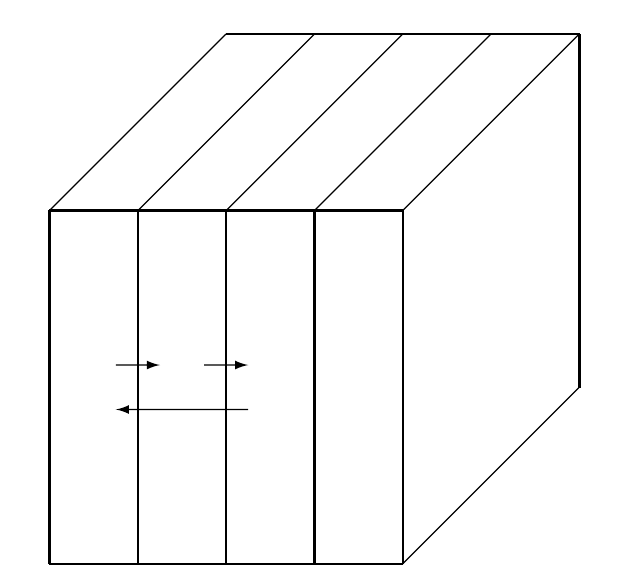
\includegraphics[width=0.5\textwidth]{figures/slices_permutation}
	\caption{Перестановка слоёв тензора}
	\label{fig:slices_permutation}
\end{figure}

В более общем смысле, пусть $A: K^{k} \to K^{k'}, B: K^{m} \to K^{m'}$ и $C: K^{n} \to K^{n'}$ являются гомоморфизмами. Пусть $t = \sum_{j=1}^{r} t_j$ с триадами $t_j = a_{j1} \otimes a_{j2} \otimes a_{j3}$. Для триад $t_j$ зададим
\[
	(A \otimes B \otimes C) t_j = A(a_{j1}) \otimes B(a_{j2}) \otimes C(a_{j3})
\]
и
\[
	(A \otimes B \otimes C) t = \sum_{j=1}^r (A \otimes B \otimes C) t_j.
\]
Также как и выше, если рассмотреть отдельный элемент $t$, то легко увидеть, что это отображение вполне определено.

Доказательство следующей леммы очевидно.
\begin{lemma}\label{lem:bi:4.4}
  $R((A \otimes B \otimes C)t) \leq R(t)$.
\end{lemma}
Равенство выполняется, если $A, B$ и $C$ изоморфизмы.

Как же выглядит тензор матричного умножения? Вспомним, что его билинейные формы задаются как
\[\label{matrix_tensor}
	Z_{\kappa \nu} = \sum\limits_{\mu=1}^{m} X_{\kappa \mu} Y_{\mu \nu}, \; 1 \leq \kappa \leq k,\; 1 \leq \nu \leq n.
\]
Элементы соответствующего тензора
\[
	\left( t_{\kappa \bar{\mu}, \mu \bar{\nu}, \nu \bar{\kappa}} \right) = t \in K^{(k \times m) \times (m \times n) \times (n \times k)}
\]
задаются как
\[
	t_{\kappa \bar{\mu}, \mu \bar{\nu}, \nu \bar{\kappa}} = \delta_{\bar{\kappa}\kappa} \delta_{\bar{\mu} \mu} \delta_{\bar{\nu} \nu},
\]
где $\delta_{ij}$ --- это дельта Кронекера --- функция равная 1, если $i=j$, и 0, если $i \neq j$. (Здесь каждое измерение тензора индексируется двумя числами, что является отражением способа нумерации элементов в матрице. Если вам так больше нравится, то можно нумеровать элементы тензора индексами $1, \dotsc, km; 1, \dotsc mn; 1, \dotsc nk$. Также были <<транспонированы>> индексы в третьем слое, чтобы тензор имел более симметричный вид.) 

Пусть $\pi = \left( 1\;2\;3 \right)$. Тогда для $t' := \pi t \in K^{(n \times k) \times (k \times m) \times (m \times n)}$ получим
\[
	\begin{array}{lcl}
		t'_{\nu \bar{\kappa}, \kappa \bar{\mu}, \mu \bar{\nu}  } & = & \delta_{\bar{\nu} \nu} \delta_{\bar{\kappa}\kappa} \delta_{\bar{\mu} \mu} \\
		& = & \delta_{\bar{\kappa}\kappa} \delta_{\bar{\mu} \mu} \delta_{\bar{\nu} \nu}\\
		& = & t_{\kappa \bar{\mu}, \mu \bar{\nu}, \nu \bar{\kappa}   }.
	\end{array}
\]
Поэтому $t' = \left\langle n,k,m \right\rangle$ (напомню, что $t = \left\langle k,m,n \right\rangle$). Ничто не мешает применить $\pi$ к $t'$, и тогда $\pi t' = \left\langle m,n,k \right\rangle$. Отсюда по лемме \ref{lem:bi:4.3} $R \left( \left\langle k, m, n \right\rangle \right) = R \left( \left\langle n, k, m \right\rangle \right) = R \left( \left\langle m, n, k \right\rangle \right)$.

Теперь пусть $t'':=\left( t_{\mu \bar{\kappa}, \nu \bar{\mu}, \kappa \bar{\nu} } \right) \in K^{(m \times k) \times (n \times m) \times (k \times n)}$. Получим, что $R(t)=R(t'')$, потому как перестановка <<внутренних>> индексов соответствует перестановке слоёв тензора.

Затем положим $\pi = (1\;2)(3)$. И пусть $t''':= \pi t'' \in K^{(n \times m) \times (m \times k) \times (k \times n)}$. Получим, что
\begin{align*}
     t'''_{\nu \bar{\mu}, \mu \bar{\kappa}, \kappa \bar{\nu}   } & = \delta_{\mu \bar{\mu} } \delta_{\kappa \bar{\kappa} } \delta_{\nu \bar{\nu} }\\
     & = t_{\bar{\kappa}\mu, \bar{\mu} \nu, \bar{\nu} \kappa}.
\end{align*}
Отсюда $R \left( \left\langle k,m,n \right\rangle \right) = R \left( \left\langle n,m,k \right\rangle \right)$. Это соответствует известному факту для матриц:
\[
	\underset{k \times m}{A} \cdot \underset{m \times n}{B} = \underset{k \times n}{C} \implies \underset{n \times m}{B^T} \cdot \underset{m \times k}{A^T} = \underset{n \times k}{C^T}.
\]

\subsection{Произведение и сумма}

Пусть $t \in K^{k \times m \times n}$ и $t' \in K^{k' \times m' \times n'}$. \textbf{Прямой суммой} $t$ и $t'$ называют тензор $s := t \oplus t' \in K^{(k+k') \times (m+m') \times (n+n')}$, задаваемый как:
\[
	s_{\kappa \mu \nu} = 
	\begin{cases}
	  t_{\kappa \mu \nu} & \text{если } 1 \leq \kappa \leq k, 1 \leq \mu \leq m, 1 \leq \nu \leq n\\
	  t'_{\kappa - k, \mu - m, \nu -n} & \parbox[t]{.6\textwidth}{если  ${k+1 \leq \kappa \leq k+k'}, {m+1 \leq \mu \leq m+m'}, {n+1 \leq \nu \leq n+n'}$} \\
	  0 & \text{иначе }
	\end{cases}
\]
\begin{figure}[H]
	\centering
    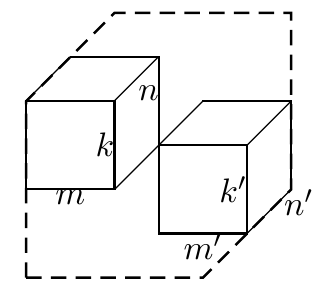
\includegraphics[width=0.25\textwidth]{figures/direct_sum}
	\caption{Прямая сумма двух тензоров}
	\label{fig:direct_sum}
\end{figure}

\begin{lemma}\label{lem:bi:4.5}
  $R \left( t \oplus t' \right) \leq R(t) + R(t')$. 
\end{lemma}
\begin{proof}
  Пусть $t = \sum_{i=1}^r u_i \otimes v_i \otimes w_i$ и $t' = \sum_{i=1}^{r'} u_i' \otimes v_i' \otimes w_i'$. Пусть
  \begin{align*}
    \widehat{u}_i & = (\underbrace{u_{i1}, \dotsc, u_{ik}}_{u_i},\underbrace{0, \dotsc, 0}_{k'})   \text{ и }\\
    \widehat{u}_i' & = (\underbrace{0, \dotsc, 0}_{k}, \underbrace{u_{i1}', \dotsc, u_{ik}'}_{u_i'}).
  \end{align*}
  и определим $\widehat{v}_i, \widehat{w}_i$ и $\widehat{v}_i', \widehat{w}_i'$ аналогично. Простые вычисления показывают, что
  \[
  	t \oplus t' = \sum_{i=1}^{r} \widehat{u}_i \otimes \widehat{v}_i \otimes \widehat{w}_i + \sum_{j=1}^{r'} \widehat{u}_j' \otimes \widehat{v}_j' \otimes \widehat{w}_j',
  \]
  то есть $R(t \oplus t') \leq r + r' = R(t) + R(t')$.
\end{proof}

\begin{reseach}[Аддитивная гипотеза Штрассена]\label{res:bi:4.1}
	Показать, что для всех тензоров $t$ и $t'$: $R(t \oplus t') = R(t) + R(t')$, то есть в лемме выше всегда имеет место равенство.
\end{reseach}

\textbf{Тензорное произведение} $t \otimes t' \in K^{kk' \times mm' \times nn'}$ двух тензоров $t \in K^{k \times m \times n}$ и $t' \in K^{k' \times m' \times n'}$ задаётся как 
\[
	t \otimes t' = \left( t_{\kappa \mu \nu} t'_{\kappa' \mu' \nu'} \right)_{\substack{
		1 \leq \kappa \leq k, \; 1 \leq \kappa' \leq k' \\
		1 \leq \mu \leq m, \; 1 \leq \mu' \leq m'\\
		1 \leq \nu \leq n, \; 1 \leq \nu' \leq n'}}
\]
\begin{figure}[H]
	\centering
    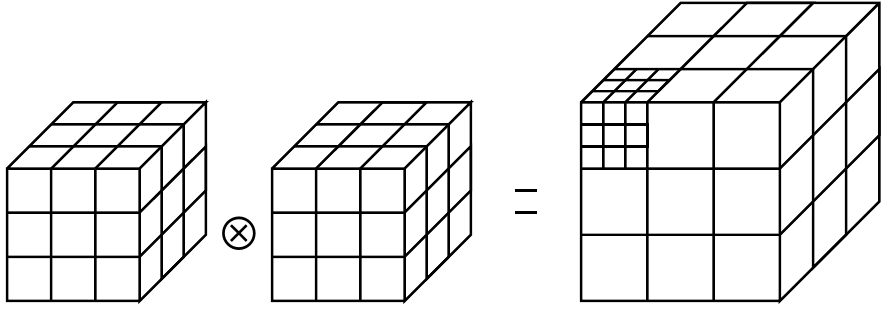
\includegraphics[width=0.75\textwidth]{figures/tensor_product}
	\caption{Тензорное произведение}
	\label{fig:tensor_product}
\end{figure}
\begin{lemma}
  $R \left( t \otimes t' \right) \leq R(t) R(t')$. 
\end{lemma}
\begin{proof}
  Пусть $t = \sum_{i=1}^r u_i \otimes v_i \otimes w_i$ и $t' = \sum_{i=1}^{r'} u_i' \otimes v_i' \otimes w_i'$. Пусть $u_i \otimes u_j' \overset{Def}{=} (u_{i \kappa} u_{j \kappa'}') \in K^{k k'}$
  Тем же образом определим $v_i \otimes v_j', w_i \otimes w_j'$. Имеем
  \begin{align*}
    (u_i \otimes u_j') \otimes (v_i \otimes v_j') \otimes (w_i \otimes w_j') & = (u_{i \kappa} u_{j \kappa'}' \cdot v_{j \mu} v_{j \mu'}' \cdot w_{i \nu} w_{j \nu'}')_{\substack{
		1 \leq \kappa \leq k, \; 1 \leq \kappa' \leq k' \\
		1 \leq \mu \leq m, \; 1 \leq \mu' \leq m'\\
		1 \leq \nu \leq n, \; 1 \leq \nu' \leq n'}} \\
		& \in K^{k k' \times m m' \times n n'} \cong K^{(k \times k') \times (m \times m') \times (n \times n')}   
  \end{align*}
  и
  \begin{align*}
    \sum_{i=1}^r \sum_{j=1}^{r'} (u_i \otimes u_j') \otimes (v_i \otimes v_j') \otimes (w_i \otimes w_j') & = 
    			\left( \sum_{i=1}^r \sum_{j=1}^{r'} u_{i \kappa} u_{j \kappa'}' v_{i \mu} v_{j \mu'}' w_{i \nu} w_{j \nu'}' \right)_{\substack{
		1 \leq \kappa \leq k, \; 1 \leq \kappa' \leq k' \\
		1 \leq \mu \leq m, \; 1 \leq \mu' \leq m'\\
		1 \leq \nu \leq n, \; 1 \leq \nu' \leq n'}}    \\
		& = \bigg( \underbrace{\left( \sum_{i=1}^r u_{i \kappa} v_{i \mu} w_{i \nu} \right)}_{t_{\kappa \mu \nu}} \cdot \underbrace{\left( \sum_{j=1}^{r'} u_{j \kappa'}' v_{j \mu'}' w_{j \nu'}' \right)}_{t_{\kappa' \mu' \nu'}'} \bigg)_{\substack{
		1 \leq \kappa \leq k, \; 1 \leq \kappa' \leq k' \\
		1 \leq \mu \leq m, \; 1 \leq \mu' \leq m'\\
		1 \leq \nu \leq n, \; 1 \leq \nu' \leq n'}}    \\
		& = t \otimes t',
  \end{align*}
  то есть $R(t \otimes  t') \leq r r' = R(t) R(t')$.
\end{proof}

Для тензорного произведения матричных умножений получим, что
\[
	\begin{array}{lcl}
		\left\langle k,m,n \right\rangle \otimes \left\langle k', m', n' \right\rangle	& = & \left( 
			\delta_{\kappa \bar{\kappa}} \delta_{\mu \bar{\mu}} \delta_{\nu \bar{\nu}} 
			\delta_{\kappa' \bar{\kappa'}} \delta_{\mu' \bar{\mu'}} \delta_{\nu' \bar{\nu'}}
		\right)\\
		& = & \left( \delta_{\kappa \bar{\kappa}} \delta_{\kappa' \bar{\kappa'}} \delta_{\mu \bar{\mu}} \delta_{\mu' \bar{\mu'}} \delta_{\nu \bar{\nu}} \delta_{\nu' \bar{\nu'}}\right)\\
		& = & \left( \delta_{(\kappa, \kappa'), (\bar{\kappa}, \bar{\kappa'})}, \delta_{(\mu, \mu'), (\bar{\mu}, \bar{\mu'})}, \delta_{(\nu, \nu'), (\bar{\nu}, \bar{\nu'})} \right)\\
		& = & \left\langle kk', mm', nn' \right\rangle
	\end{array}
\]

Таким образом, тензорное произведение двух матричных тензоров будет снова матричным тензором, но больших размеров, что соответствует тождеству для произведений Кронекера
\[
	(A \otimes B)(A' \otimes B') = (AA' \otimes BB').
\]

\begin{theorem}\label{th:4.7}
	Для всех $k,m,n$ получим, что $(kmn)^{\omega/3} \leq R(\left\langle k,m,n \right\rangle)$.
\end{theorem}
\begin{proof}
	Пусть $R(\left\langle k,m,n \right\rangle) \leq r$, тогда $R(\left\langle n,k,m \right\rangle) \leq r$ и $R(\left\langle m,n,k \right\rangle) \leq r$. Поэтому
	\[
		R(\underbrace{\left\langle k,m,n \right\rangle \otimes \left\langle n,k,m \right\rangle \otimes \left\langle m,n,k \right\rangle}_{=\left\langle kmn, kmn, kmn \right\rangle}) \leq r^3.
	\]
	Положив, $M=kmn$ получим $R(\langle M , M, M \rangle) \leq r^3$. Тогда для всех $N \geq 1$, при помощи дополнения до
следующей наибольшей степени $M^i$ числа $M$,
	\[
		R(\left\langle N,N,N \right\rangle) \leq R(\left\langle M^i, M^i, M^i \right\rangle) \leq r^{3i} = (M^{3 \log_M r})^i = (M^i)^{3 \log_M r} = O(N^{3 \log_M r})
	\]
	 Поэтому 
	  \begin{align*}
	    \omega & \leq 3 \log_M r   \\
	    M^{\omega/3} & \leq r \\
	    (k m n)^{\omega/3} & \leq r.
	  \end{align*} 
	По определению $R(\left\langle k,m,n \right\rangle)$ является положительным целым, и так как $R(\left\langle k,m,n \right\rangle) \leq R(\left\langle k,m,n \right\rangle)$ то получим, что $(k m n)^{\omega/3} \leq R(\left\langle k,m,n \right\rangle)$. Это будет эквивалентно $\omega \leq \frac{\log R(\left\langle k,m,n \right\rangle)}{\log (kmn)^{1/3}}$.
\end{proof}

Стандартное применение теоремы \ref{th:4.7} будет следующим: допустим, что доказано $R(\left\langle 2,2,2 \right\rangle) \leq 7$ (в данном случае это результат Штрассена 1969 года \cite{Strassen:1969}), отсюда будет следовать нетривиальная верхняя оценка на экспоненту матричного умножения 
\[
	\omega \leq 3 \log_{2^3} 7 = \log_2 7 \approx 2.81.
\]











	\section{Граничный ранг}

\begin{definition}
  \textbf{Полунепрерывность} функции является более слабым свойством, чем непрерывность. \textbf{Функция полунепрерывна сверху в точке}, если значения функции в близких точках не сильно превышают значение функции в ней. \textbf{Функция полунепрерывна снизу в точке}, если значения функции в близких точках не сильно меньше значения функции в ней.
\end{definition}
Над $\mathbb{R}$ и $\mathbb{C}$ матричный ранг является полунепрерывным. Пусть
\[
	\mathbb{C}^{n \times n} \ni A_j \to A = \lim_{j \to \infty} A_j.
\]
Будем обозначать ранг матрицы $M$ через $rk(M)$. Если для всех $j$ верно $rk(A_j) \leq r$, то $rk(A) \leq r$. Неравенство $rk(A_j) \leq r$ означает, что все $(r+1) \times (r+1)$-миноры обнуляются. (Напомню, что $k \times k$-минором матрицы $A$ называют определитель квадратной матрицы $B$, составленной из элементов матрицы $A$, стоящих на пересечении каких-то $k$ столбцов и каких-то $k$ строк.) Но так как миноры являются непрерывными функциями, то все $(r+1) \times (r+1)$-миноры $A$ также обнуляются.

Тоже самое будет верно для трёхмерных тензоров. Рассмотрим произведение многочленов первой степени от одной переменной по модулю $X^2$:
\[
	(a_0+a_1 X)(b_0 + b_1 X)= a_0 b_0 + (a_1 b_0 + a_0 b_1)X + a_1 b_1 X^2.
\]
Тензор, соответствующий двум билинейным формам $a_0 b_0$ и $a_1 b_0 + a_0 b_1$, имеет ранг 3:
\begin{align*}
  \begin{array}{|c|c|}
  \hline
  1 & 0 \\
  \hline
  0 & 0\\
  \hline
 \end{array}  & \;\;\;\;
 \begin{array}{|c|c|}
  \hline
  0 & 1 \\
  \hline
  1 & 0\\
  \hline
 \end{array} 
\end{align*}

Напомню, что ранги билинейной задачи и её тензора совпадают. В данном случае мы решаем билинейную задачу $F = \left\{ a_0 b_0, a_1 b_0 + a_0 b_1 \right\}$. Чтобы найти её ранг, нужно узнать скольких произведений вида
\[
	P_{\lambda} = \left( \alpha_{\lambda 0} a_0 + \alpha_{\lambda 1} a_1 \right) \cdot \left( \beta_{\lambda 0} b_0 + \beta_{\lambda 1} b_1 \right), 1 \leq \lambda \leq \ell
\]
будет достаточно, чтобы $F$ была в линейной оболочке $lin_{\mathbb{C}}\left\{ P_1, \dotsc, P_{\ell} \right\}$, то есть чему равно число $\ell$.

Чтобы показать, что ранг $F$ больше или равен 3, будем использовать метод подстановок. Сначала положим $a_0=0, b_0=1$. Тогда нам всё ещё нужно вычислить $a_1$, значит есть произведение, зависящее от $a_1$. Скажем, пусть один из его множителей равен $\alpha_{\lambda 0} a_0 + \underbrace{\alpha_{\lambda 1} a_1}_{\neq 0}$. Тогда, заменив $a_1$ на $- \frac{\alpha_{\lambda 0}}{\alpha_{\lambda 1}} a_0$, сможем избавиться от одного произведения. После этого мы будем решать более простую задачу $F' = \left\{ a_0 b_0, -\frac{\alpha_{\lambda 0}}{\alpha_{\lambda 1}}a_0 b_0 + a_0 b_1 \right\}$. Если мы присвоим $a_0=1, b_0=0$, то всё ещё будем вычислять $b_1$. Мы сможем избавиться от другого произведения, выполнив аналогичную подстановку для $b_1$, а именно пусть один из множителей равен $\beta_{\lambda 0} b_0 + \beta_{\lambda 1} b_1$, тогда подставим $-\frac{\beta_{\lambda 0}}{\beta_{\lambda 1}} b_0$ вместо $b_1$.  После всего этого мы всё ещё должны вычислить $F'' = \left\{ a_0 b_0  \right\} $, что требует одного произведения. Очевидно, что ранг будет меньше равен 3, так как 
\[
	F  = \left\{ a_0 b_0, a_1 b_0 + a_0 b_1 \right\} \subseteq lin_{\mathbb{C}}\left\{ P_1 = a_0 b_0, P_2 = a_1 b_0, P_3 = a_0 b_1 \right\}.
\] 

\phantomsection
\label{border_rank_2}
Однако мы можем аппроксимировать тензор, упомянутый выше, с помощью тензоров c рангом два. Пусть
\[
	t(\varepsilon)=(1,\varepsilon) \otimes (1,\varepsilon) \otimes (0, \frac{1}{\varepsilon}) + (1,0) \otimes (1,0) \otimes (1, -\frac{1}{\varepsilon}).
\]

Очевидно, что $t(\varepsilon)$ имеет ранг два для любого $\varepsilon > 0$. Слои $t(\varepsilon)$ будут выглядеть следующим образом
\begin{align*}
  \begin{array}{|c|c|}
  \hline
  1 & 0 \\
  \hline
  0 & 0\\
  \hline
 \end{array}  & \;\;\;\;
 \begin{array}{|c|c|}
  \hline
  0 & 1 \\
  \hline
  1 & \varepsilon\\
  \hline
 \end{array} 
\end{align*}
Поэтому $t(\varepsilon) \to t$, когда $\varepsilon \to 0$.

Бини и др. \cite{Bini} использовали этот эффект, чтобы разработать лучший алгоритм для перемножения матриц. Они начали со следующего частичного матричного умножения:
\[
	\begin{pmatrix}
	  x_{11} & x_{12}\\
	  x_{21} & x_{22} 
	\end{pmatrix}
	\left( 
	\begin{array}{c|c}
	  y_{11} & y_{12}\\
	  y_{21} & \cancel{y_{22}}
	\end{array}
	 \right)
	 =
	 \left( 
	\begin{array}{c|c}
	  z_{11} & z_{12}\\
	  z_{21} & \cancel{z_{22}}
	\end{array}
	 \right),
\]
где они хотели вычислить только три элемента результирующей матрицы. Получаем, что $R(\left\{ z_{11}, z_{12}, z_{21} \right\})=6$, хотя можно приблизительно вычислить $\left\{ z_{11}, z_{12}, z_{21} \right\}$, используя только пять умножений.

То что ранг равен шести, можно показать используя метод подстановок. Рассмотрим $z_{12}$. Ясно, что он зависит от $y_{12}$, поэтому существует произведение, у которого один из множителей равен $y_{12} + \ell(y_{11}, y_{21}, y_{22})$, где $\ell$ --- это линейная форма. Подстановка $y_{12} \to -\ell(y_{11}, y_{21}, y_{22})$ повлияет только на $z_{12}$. После неё мы всё ещё вычисляем $\overline{z_{12}}=x_{11}(-\ell(y_{11},y_{21},y_{22})) + x_{12}y_{22}$. Билинейная форма $\overline{z_{12}}$ всё ещё зависит от $y_{22}$. Поэтому можно снова выполнить подстановку $y_{22} \to -\ell'(y_{11}, y_{21})$. Это уничтожит два произведения, и мы всё ещё вычисляем $z_{11},z_{21}$.

Рассмотрим следующие пять произведений:
\begin{align*}
  p_1 & = (x_{12} + \varepsilon x_{22})   y_{21}\\
  p_2 & = x_{11} (y_{11} + \varepsilon y_{12})\\
  p_3 & = x_{12} (y_{12} + y_{21} + \varepsilon y_{22})\\
  p_4 & = (x_{11} + x_{12} + \varepsilon x_{21}) y_{11}\\
  p_5 & = (x_{12} + \varepsilon x_{21}) (y_{11} + \varepsilon y_{22})
\end{align*}
Получим, что
\begin{align*}
  \varepsilon z_{11}   & = \varepsilon p_1 + \varepsilon p_2 + O(\varepsilon^2)\\
  \varepsilon z_{12} & = p_2 - p_4 + p_5 + O(\varepsilon^2)\\
  \varepsilon z_{21} & = p_1 - p_3 + p_5 + O(\varepsilon^2)
\end{align*}

Теперь возьмём вторую копию того же частичного матричного умножения с новыми переменными. Используя эти две копии, можно перемножать $2 \times 2$ и $2 \times 3$-матрицы (при помощи отождествления некоторых переменных в копии). Поэтому мы можем приблизительно вычислить $\left\langle 2,2,3 \right\rangle$ с помощью 10 умножений. Если бы приближение было бы так же хорошо как точное вычисление, то мы получили бы из этого $\omega \leq 2.79$.

Формализуем концепцию приближения. Пусть $K$ --- поле, и $\widehat{K}:=K[[\varepsilon]]$. (Напомню, что $K[[\varepsilon]]$ обозначает множество всех формальных степенных рядов от переменной $\varepsilon$.) Пусть теперь $\varepsilon$ обозначает неизвестную, а не малую величину как в начале подраздела.

\begin{definition}\label{def:bi:5.1}
	Пусть $h \in \mathbb{N}, t \in K^{k \times m \times n}$.
	\begin{enumerate}
		\item $R_h(t) = \min\{ r \mid \exists u_\rho \in K[\varepsilon]^k, v_\rho \in K[\varepsilon]^m, w_\rho \in K[\varepsilon]^n : \sum_{\rho=1}^r u_{\rho} \otimes v_{\rho} \otimes w_{\rho} = \varepsilon^h t + O(\varepsilon^{h+1}) \}$
		\item $\underline{R}(t)=\min\limits_h R_h(t)$, $\underline{R}(t)$ называется \textbf{граничным рангом} $t$.
	\end{enumerate}
\end{definition}

\begin{remark}\label{rem:bi:5.2}\ 
	\begin{enumerate}
		\item $R_0(t)= R(t)$
		\item $R_0(t) \geq R_1(t) \geq \dotsb = \underline{R}(t)$
		\item Для $R_h$ в $u_{\rho}, v_{\rho}, w_{\rho}$ достаточно будет рассматривать степени вплоть до $\varepsilon^h$.
	\end{enumerate}
\end{remark}

\begin{theorem}\label{th:bi:5.3}
  Пусть $t \in K^{k \times m \times n}, t' \in K^{k' \times m' \times n'}$. Мы имеем
  \begin{enumerate}
       \item $\forall \pi \in S_3: R_h(\pi t) = R_h(t)$.\label{itm:1:th:bi:5.3}
       \item $R_{\max \left\{ h, h' \right\}}(t \oplus t') \leq R_h(t) + R_{h'}(t')$.\label{itm:2:th:bi:5.3}
       \item $R_{h+h'}(t \otimes t') \leq R_{h}(t) \cdot R_{h'}(t')$.\label{itm:3:th:bi:5.3}
  \end{enumerate} 
\end{theorem}
\begin{proof}\ 
  \begin{enumerate}
       \item Очевидно.
       \item Без ограничения общности положим $h \geq h'$. Существуют приблизительные вычисления такие, что
       \begin{align*}
         \sum_{\rho=1}^r u_{\rho} \otimes v_{\rho}  \otimes w_{\rho} & = \varepsilon^h t + O(\varepsilon^{h+1}) \\
         \sum_{\rho=1}^{r'} \varepsilon^{h-h'} u_{\rho}' \otimes v_{\rho}'  \otimes w_{\rho}' & = \varepsilon^{h-h'}\left( \varepsilon^{h'} t' + O(\varepsilon^{h' + 1}) \right) = \varepsilon^h t' + O(\varepsilon^{h+1})
       \end{align*}
       Теперь можно объединить два эти вычисления, так же как делали раньше в случае рангов.
       \item Пусть $t=(t_{ij \ell})$ и $t'=(t_{i' j' \ell'}')$. Имеем $t \otimes t' = (t_{i j \ell} \cdot t_{i' j' \ell'}') \in K^{k k' \times m m' \times n n'}$. Возьмём два приблизительных вычисления для $t$ и $t'$, наподобие тех, что были выше. Если смотреть на них, как на точные вычисления в поле $K[[\varepsilon]]$, то их тензорное произведение вычисляется следующим образом:
       \begin{align*}
         T = \varepsilon^h t + \varepsilon^{h+1} \widehat{t}, &\;\;\;  T' = \varepsilon^{h'} t' + \varepsilon^{h' + 1} \widehat{t}',
       \end{align*}
       где $\widehat{t} \in K[\varepsilon]^{k \times m \times n}$ и $\widehat{t}' \in K[\varepsilon]^{k' \times m' \times n'}$. Их тензорное произведение будет вычислять:
       \begin{align*}
         T \otimes T' & = (\varepsilon^h t_{ij \ell} + \varepsilon^{h+1} \widehat{t}_{ij \ell})(\varepsilon^{h'} t_{i'j'\ell'}' + \varepsilon^{h' + 1}\widehat{t}_{i'j'\ell'}')\\
         & = (\varepsilon^{h+h'}t_{ij \ell} t_{i'j'\ell'}' + O(\varepsilon^{h+h'+1}))\\
         & = \varepsilon^{h+h'} t \otimes t' + O(\varepsilon^{h + h' + 1})
       \end{align*}
       Но это будет приблизительным вычислением для $t \otimes t'$. \qedhere
  \end{enumerate}
\end{proof}

Следующая лемма покажет, что можно превращать приблизительные вычисления в точные.
\begin{lemma}\label{lem:bi:5.4}
  Существует константа $c_h$ такая, что для всех $t$: $R(t) \leq c_h R_h(t)$. $c_h$ зависит полиномиально от $h$, в частности $c_h \leq \binom{h+2}{2}$.
\end{lemma}
\begin{remark}
  \textit{(Наилучшая оценка для $c_h$)} Над конечными полями даже $c_h=1 + 2h$ будет достаточно.
\end{remark}
\begin{proof}
  Пусть $t$ будет тензором с граничным рангом $r$ и пусть
  \[
  	\sum_{\rho=1}^r \underbrace{\left( \sum_{\alpha=0}^h \varepsilon^\alpha u_{\rho \alpha} \right)}_{\in K[\varepsilon]^k} \otimes \left( \sum_{\beta=0}^h \varepsilon^\beta v_{\rho \beta} \right) \otimes \left( \sum_{\gamma=0}^h \varepsilon^\gamma w_{\rho \gamma} \right) = \varepsilon^h t + O(\varepsilon^{h+1}).
  \]
  \begin{figure}[H]
	\centering
    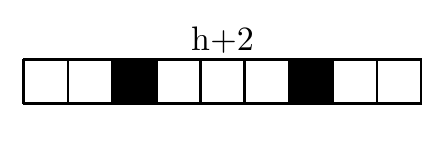
\includegraphics[width=0.3\textwidth]{figures/decomposition}
	\caption{Выбрав два из $h+2$ квадратов, получим разложение $h$ на три части. Поэтому существует всего $\binom{h+2}{2}$ таких разложений.}
	\label{fig:bi:5.1}
  \end{figure}
  Левую часть уравнения можно переписать следующим образом:
  \[
  	\sum_{\rho=1}^r \sum_{\alpha=0}^h \sum_{\beta=0}^h \sum_{\gamma=0}^h \varepsilon^{\alpha+\beta+\gamma} u_{\rho \alpha} \otimes v_{\rho \beta} \otimes w_{\rho \gamma}.
  \]
  Сравнивая коэффициенты при степенях $\varepsilon$, увидим, что $t$ является суммой всех $u_{\rho \alpha} \otimes v_{\rho \beta} \otimes w_{\rho \gamma}$, где $\alpha + \beta + \gamma = h$. Поэтому всё, что необходимо, это вычислить $\binom{h+2}{2}$ произведений.
\end{proof}

В качестве первой попытки использования полученных результатов сделаем следующее:
\begin{align*}
  R_1(\left\langle 2,2,3 \right\rangle)   & \leq 10 \\
  R_1(\left\langle 3,2,2 \right\rangle)   & \leq 10 & (\text{Теорема } \ref{th:bi:5.3}.\ref{itm:1:th:bi:5.3})\\
  R_1(\left\langle 2,3,2 \right\rangle)   & \leq 10 \\
  R_3(\left\langle 12,12,12 \right\rangle)& \leq 1000 & (\text{Теорема } \ref{th:bi:5.3}.\ref{itm:3:th:bi:5.3})\\
  \implies R(\left\langle 12,12,12 \right\rangle) & \leq \binom{3+2}{2} \cdot 1000 = 10 \cdot 1000 = 10000
\end{align*}
Но легко можно получить, что $R(\left\langle 12,12,12 \right\rangle) \leq 12^3 = 1728$. Оказывается, что лучше сначала возвести в тензорную степень, а затем превратить приближённое вычисление в точное.
\begin{theorem}\label{th:bi:5.6} 
  Если $\underline{R}(\left\langle k,m,n \right\rangle) \leq r$, то $\omega \leq 3 \log_{kmn} r$.
\end{theorem}
\begin{proof}
  Пусть $M=kmn$ и пусть $R_h(\left\langle k,m,n \right\rangle) \leq r$. По теореме \ref{th:bi:5.3} получим, что $R_{3h}(\left\langle M,M,M \right\rangle) \leq r^3$ и $R_{3hs}(\left\langle M^s, M^s, M^s \right\rangle) \leq r^{3s}$ для всех $s$. По лемме \ref{lem:bi:5.4} это даст $R(\left\langle M^s, M^s, M^s \right\rangle) \leq c_{3hs} r^{3s}$. Поэтому
  \begin{align*}
    \omega  & \leq  \log_{M^s} (c_{3hs} r^{3s})\\
    & = 3s \log_{M^s}(r) + \log_{M^s}(c_{3hs})\\
    & = 3 \log_M(r) + \underbrace{\frac{1}{s} \log_M(\text{ многочлен от } s)}_{\to 0 \text{ при } s \to \infty}.
  \end{align*}
  Так как $\omega$ является инфимумом, то получим $\omega \leq 3 \log_M(r)$.
\end{proof}

\begin{corollary}
  $\omega \leq 2.79 \dotso$
\end{corollary}

	\section{$\tau$-теорема}

В этом разделе мы рассмотрим прямые суммы матричных тензоров, а именно суммы вида $\left\langle k,1,n \right\rangle \oplus \left\langle 1,m,1 \right\rangle$. Первое слагаемое является произведением вектора длины $k$ и вектора длины $n$, которое даёт матрицу ранга 1. Второе слагаемое --- это скалярное произведение двух векторов длины $m$.

\begin{remark}\label{rem:bi:6.1}\ 
  	\begin{enumerate}
	     \item $R(\left\langle k,1,n \right\rangle \oplus \left\langle 1,m,1 \right\rangle) = k \cdot n + m$
	     \item $\underline{R}(\left\langle k,1,n \right\rangle) = k \cdot n$ и $\underline{R}(\left\langle 1,m,1 \right\rangle) = m$
	     \item $\underline{R}(\left\langle k,1,n \right\rangle \oplus \left\langle 1,m,1 \right\rangle) \leq k \cdot n + 1$, где $m = (n-1)(k-1)$. 
	\end{enumerate}	
\end{remark}

Первое утверждение можно доказать, используя метод подстановок. Мы сначала заменяем $m$ переменных, принадлежащих одному из векторов $\left\langle 1,m,1 \right\rangle$. Затем мы устанавливаем переменные другого вектора в ноль. Мы всё ещё вычисляем $\left\langle k,1,n \right\rangle$.

Для второго утверждения достаточно заметить, что оба тензора состоят из $kn$ и $m$ линейно независимых слоёв соответственно.

Для третьего утверждения мы только докажем случай $k=n=3$. Из него общее построение станет очевидным. Итак мы хотим вычислить $a_i b_j$ для $1 \leq i,j \leq 3$ и $\sum_{\mu=1}^4 u_{\mu} v_{\mu}$. Рассмотрим следующие произведения
\begin{align*}
  p_1 & = (a_1 + \varepsilon u_1)(b_1 + \varepsilon v_1)\\
  p_2 & = (a_1 + \varepsilon u_2)(b_2 + \varepsilon v_2)\\
  p_3 & = (a_2 + \varepsilon u_3)(b_1 + \varepsilon v_3)\\    
  p_4 & = (a_2 + \varepsilon u_4)(b_2 + \varepsilon v_4)\\
  p_5 & = (a_3 - \varepsilon u_1 - \varepsilon u_3)b_1\\
  p_6 & = (a_3 - \varepsilon u_2 - \varepsilon u_4)b_2\\
  p_7 & = a_1 (b_3 - \varepsilon v_1 - \varepsilon v_2)\\
  p_8 & = a_2 (b_3 - \varepsilon v_3 - \varepsilon v_4)\\
  p_9 & = a_3 b_3
\end{align*}
Эти девять произведений очевидно вычисляют $a_i b_j, \; 1 \leq i,j \leq 3$. Более того
\[
	\varepsilon^2 \sum_{\mu=1}^4 u_{\mu} v_{\mu} = p_1 + \dotsb + p_9 - (a_1 + a_2 + a_3)(b_1 + b_2 + b_3)
\]
Таким образом десяти произведений оказывается достаточным, чтобы приближённо вычислить $\left\langle 3,1,3 \right\rangle \oplus \left\langle 1,4,1 \right\rangle$.

Второе и третье утверждения вместе показывают, что аддитивная гипотеза \ref{res:bi:4.1} не верна для граничного ранга. Мы попытаемся использовать это следующим образом.

\begin{definition}\label{def:bi:6.2}
     Пусть $t \in K^{k \times m \times n}$ и $t' \in K^{k' \times m' \times n'}$.
	\begin{enumerate}
	     \item $t$ называется \textbf{ограничением} $t'$, если существуют гомоморфизмы $\alpha: K^{k'} \to K^{k}, \beta: K^{m'} \to K^{m}$ и $\gamma: K^{n'} \to K^{n}$ такие, что $t = (\alpha \otimes \beta \otimes \gamma)t'$. Будем писать $t \leq t'$.
	     \item $t$ и $t'$ будут изоморфными, если $\alpha, \beta, \gamma$ --- изоморфизмы ($t \cong t'$).
	\end{enumerate}
\end{definition}

В дальнейшем $\left\langle r \right\rangle$ будет обозначать тензор в $K^{r \times r \times r}$, который имеет 1 в позициях $(\rho, \rho, \rho)$ и 0 во всех остальных. Этот тензор соответствует $r$ билинейным формам $x_{\rho} y_{\rho}, 1 \leq \rho \leq r$ ($r$ независимых произведений)

\begin{lemma}\label{lem:bi:6.3}
  $R(t) \leq r \iff t \leq \left\langle r \right\rangle$
\end{lemma}
\begin{proof}\ \\
  ($\Longleftarrow$) Немедленно из леммы \ref{lem:bi:4.4}.\\
  ($\Longrightarrow$) $\left\langle r \right\rangle = \sum_{\rho = 1}^r e_{\rho} \otimes e_{\rho} \otimes e_{\rho}$, где $e_{\rho}$ --- это $\rho$-ый единичный вектор. Если ранг $t$ меньше равен $r$, то мы можем записать $t$ как сумму $r$ триад
\[
	t = \sum_{\rho=1}^r u_{\rho} \otimes v_{\rho} \otimes w_{\rho}.
\]
Определим три гомоморфизма:
\begin{align*}
	\alpha & \text{ задаётся как } e_{\rho} \mapsto u_{\rho}; \; 1 \leq \rho \leq r\\
	\beta & \text{ задаётся как } e_{\rho} \mapsto v_{\rho}; \; 1 \leq \rho \leq r\\
	\gamma & \text{ задаётся как } e_{\rho} \mapsto w_{\rho}; \; 1 \leq \rho \leq r\\
\end{align*}
По построению
\[
	(\alpha \otimes \beta \otimes \gamma)\left\langle r \right\rangle = \sum_{\rho=1}^r \underbrace{\alpha(e_{\rho})}_{=u_{\rho}} \otimes \underbrace{\beta(e_{\rho})}_{=v_{\rho}} \otimes \underbrace{\gamma(e_{\rho})}_{=w_{\rho}} = t,
\]
что завершает доказательство.
\end{proof}

\begin{observation}\ 
  \begin{enumerate}
       \item $t \otimes t' \cong t' \otimes t$
       \item $t \otimes (t' \otimes t'') \cong (t \otimes t') \otimes t''$
       \item $t \oplus t' \cong t' \oplus t$
       \item $t \oplus (t' \oplus t'') \cong (t \oplus t') \oplus t''$
       \item $t \otimes \left\langle 1 \right\rangle \cong t$
       \item $t \oplus \left\langle 0 \right\rangle \cong t$
       \item $t \otimes (t' \oplus t'') \cong t \otimes t' \oplus t \otimes t''$
  \end{enumerate}
\end{observation}

Выше $\left\langle 0 \right\rangle$ обозначает пустой тензор в $K^{0 \times 0 \times 0}$. Поэтому тензоры (точнее классы изоморфизмов тензоров) образуют полукольцо. От кольца оно отличается тем, что не требуется существование обратного по сложению элемента. Например, полукольцом будет множество натуральных чисел $\mathbb{N}$. (Замечание: Если два тензора изоморфны, то они живут в одном пространстве $K^{k \times m \times n}$. Если $t$ --- любой тензор, и $n$ --- тензор заполненный одними нулями, то $t$ не изоморфен $t \oplus n$. Но с точки зрения вычислений эти тензоры \textbf{одинаковы}. Поэтому будет удобно использовать более широкое понятие эквивалентности. Будем говорить, что два тензоры $t$ и $t'$ изоморфны, если существуют тензоры $n$ и $n'$, состоящие из одних нулей, такие, что $t \oplus n$ и $t' \oplus n'$ изоморфны.) 

Основным результатом из этого раздела будет следующая теорема за авторством Шёнхаге \cite{Schonhage81}. В литературе она часто называется $\tau$-теоремой, потому что $\tau$ играет важную роль в оригинальном доказательстве. В нашем доказательстве её роль скромнее.

\begin{theorem}[$\tau$-теорема Шёнхаге]\label{th:bi:6.4} Если $\brank{\bigoplus_{i=1}^p \mt{k_i, m_i, n_i}} \leq r$, где $r > p$, то $\omega \leq 3 \tau$, где $\tau$ определена следующим образом
\[
	\sum_{i=1}^p (k_i m_i n_i)^{\tau} = r.
\]
Если не использовать $\tau$, то утверждение будет иметь следующий вид
\[
	\brank{\bigoplus_{i=1}^p \mt{k_i, m_i, n_i}} \leq r \implies \sum_{i=1}^p (k_i m_i n_i)^{\omega/3} \leq r.
\]
\end{theorem}

\begin{notation}
  Пусть $f \in \mathbb{N}$, $t$ --- это тензор. $f \odot t \overset{Def}{=} \underbrace{t \oplus \dotsb \oplus t}_{f \text{ раз }}$.
\end{notation}

\begin{lemma}\label{lem:bi:6.5} 
	Если $R(f \odot \mt{k, m, n}) \leq g$, то $\omega \leq 3 \cdot \frac{\log \ceilfrac{g}{f}}{\log (kmn)}$.
\end{lemma}
\begin{proof}
 	Сначала покажем, что для всех $s$, $R(f \odot \mt{k^s, m^s, n^s}) \leq \ceilfrac{g}{f}^s \cdot f$.

	Доказательство индукцией по $s$: Если $s=1$, то это просто условие леммы.\\
	$s \to s+1$: Имеем
	\begin{align*}
		f \odot \mt{k^{s+1}, m^{s+1}, n^{s+1}} & = \underbrace{(f \odot \mt{k, m, n})}_{\leq \mt{g}} \otimes \mt{k^s, m^s, n^s}\\
		& \leq \mt{g} \otimes \mt{k^s, m^s, n^s}\\
		& = g \odot \mt{k^s, m^s, n^s}
	\end{align*}
	Поэтому
	\begin{align*}
		\rank{f \odot \mt{k^{s+1}, m^{s+1}, n^{s+1}}} & \leq \rank{g \odot \mt{k^s, m^s, n^s}}\\
		& \rank{ \ceilfrac{g}{f} \cdot f \odot \mt{k^s, m^s, n^s}}\\
		& = \ceilfrac{g}{f} \ceilfrac{g}{f}^s  f\\
		& = \ceilfrac{g}{f}^{s+1} f
	\end{align*}
	Это доказывает утверждение. Теперь используем это утверждение, чтобы доказать лемму: 
	\[
		R(\mt{k^s, m^s, n^s}) \leq R(f \odot \mt{k^s, m^s, n^s}) = \ceilfrac{g}{f}^s \cdot f	
	\]
	означает, что по теореме \ref{th:4.7}
	\[
		\omega \leq 3 \frac{\log \ceilfrac{g}{f}^s f}{\log (kmn)^s} = \frac{3s \log \ceilfrac{g}{f} + 3 \log f}{s \cdot \log (kmn)} = \frac{3 \log \ceilfrac{g}{f} + \overbrace{\frac{3}{s} \log f}^{\to 0 \text{ при } s \to \infty}}{\log (kmn)}.
	\]
	Так как $\omega$ является инфимумом, получим $\omega \leq \frac{3 \log \ceilfrac{g}{f}}{\log(kmn)}$.
\end{proof}

\begin{proof}[Доказательство теоремы \ref{th:bi:6.4}]
	Существует $h$ такой, что
	\[
		R_h (\bigoplus_{i=1}^p \left\langle k_i, m_i, n_i \right\rangle) \leq r.
	\]
	Взяв тензорную степень и используя факт, что тензоры образуют полукольцо, получим
	\[
		R_{hs} \left( \bigoplus_{\sigma_1 + \dotsb + \sigma_p = s} \frac{s!}{\sigma_1! \dotsm \sigma_p!} \odot \left\langle \underbrace{\prod_{i=1}^p k_i^{\sigma_i}}_{=k'}, \underbrace{\prod_{i=1}^p m_i^{\sigma_i}}_{=m'}, \underbrace{\prod_{i=1}^p n_i^{\sigma_i}}_{=n'} \right\rangle \right) \leq r^s.
	\]
	$k', m', n'$ зависят от $\sigma_1, \dotsc, \sigma_p$. Затем превратим приближённое вычисление в точное и получим
	\[
		R \left( \bigoplus_{\sigma_1 + \dotsb + \sigma_p = s} \frac{s!}{\sigma_1! \dotsm \sigma_p!} \odot \left\langle k', m', n' \right\rangle \right) \leq r^s \cdot \underbrace{c_{hs}}_{\text{многочлен от } h \text{ и } s}.
	\]
	Определим $\tau$ как $\sum\limits_{\sigma_1 + \dotsb + \sigma_p = s} \underbrace{\frac{s!}{\sigma_1! \dotsm \sigma_p!} (k' m' n')^{\tau}}_{=(1)} = r^s$.
	
	Зафиксируем $\sigma_1, \dotsc, \sigma_p$ такими, что $(1)$ максимально. Тогда $k', m'$ и $n'$ будут константами. Чтобы применить лемму \ref{lem:bi:6.5}, зададим
	\begin{align*}
		f & = \frac{s!}{\sigma_1! \dotsm \sigma_p!} < p^s,\\
		g & = r^s \cdot c_{hs}\\
		k & = k', \; m = m', \; n = n'.   
	\end{align*}
	Число всех $\vec{\sigma}$, где $\sigma_1 + \dotsb + \sigma_p = s$ равно
	\[
		\dbinom{s + p - 1}{p-1} = \frac{s+p-1}{p-1} \cdot \frac{s+p-2}{p-2} \dotso \leq (s+1)^{p-1}.
	\]
	Таким образом
	\[
		f \cdot (kmn)^{\tau} \geq \frac{r^s}{(s+1)^{p-1}}.
	\]
	Мы получим, что
	\[
		\left\lceil \frac{g}{f} \right\rceil \leq \frac{r^s \cdot c_{hs}}{f} + 1 \leq (kmn)^{\tau} \cdot (s+1)^{p-1} \cdot c_{hs}.
	\]
	Более того
	\begin{equation}\label{eq:bi:6.1}
		(kmn)^{\tau} \geq \frac{r^s}{(s+1)^{p-1} f} \geq \frac{r^s}{(s+1)^{p-1} p^s}.
	\end{equation}
	Заметив, что если ранг прямой суммы матричный тензоров меньше равен $g$, то тогда и ранг наибольшего слагаемого будет меньше равен $g$, то есть
	\[
		R(f \odot \left\langle k,m,n \right\rangle) \leq g,
	\]
	и применив лемму \ref{lem:bi:6.5}, получим
	\begin{align*}
		\omega & \leq 3 \frac{\tau \log(kmn) + (p-1) \log(s+1) + \log(c_{hs})}{\log(kmn)}   \\
		& = 3 \tau + \frac{(p-1) \log(s+1) + \log(c_{hs})}{\log(kmn)} \underset{s \to \infty}{\to} 3 \tau,
	\end{align*}
	потому что $\log(kmn) \geq \frac{1}{\tau} s \underbrace{(\log r - \log p)}_{> 0} - O(\log s)$ согласно неравенству \eqref{eq:bi:6.1}.
\end{proof}

Используя пример из начала этого раздела с $k=4$ и $n=4$, получим следующую оценку из $\tau$-теоремы.
\begin{corollary}
	$\omega < 2.55$.
\end{corollary}






























	\section{Лазерный метод Штрассена}

Рассмотрим следующий тензор
\[
	\str = \sum_{i=1}^q \left(\underbrace{e_i \otimes e_0 \otimes e_i}_{\mt{q,1,1}} + \underbrace{e_0 \otimes e_i \otimes e_i}_{\mt{1,1,q}} \right)
\]
Этот тензор подобен $\mt{1,2,q}$, только <<направления>> этих двух скалярных произведений не одинаковы. Однако тензор Штрассена может быть очень эффективно приближен. Мы имеем
\[
	\sum_{i=1}^q (e_0 + \varepsilon e_i) \otimes (e_0 + \varepsilon e_i) \otimes e_i 
	= \sum_{i=1}^q e_0 \otimes e_0 \otimes e_i + \varepsilon \sum_{i=1}^q \left( e_i \otimes e_0 \otimes e_i + e_0 \otimes e_i \otimes e_i \right) + O(\varepsilon^2)
\]
Если мы вычтем триаду $e_i \otimes e_i \otimes \sum_{i=1}^q e_i$, мы получим приближение $\str$. Таким образом $\brank{\str} \leq q+1$.

\begin{definition}\label{def:bi:7.1}
	Пусть $t \in K^{k \times m \times n}$ является тензором. Пусть множества $I_i, J_j, L_{\ell}$ такие, что:
	\begin{align*}
		1 \leq i \leq p: & \; I_i \subseteq \left\{ 1, \dotsc, k \right\}   \\
		1 \leq j \leq q: & \; J_j \subseteq \left\{ 1, \dotsc, m \right\}   \\
		1 \leq \ell \leq s: & \; L_{\ell} \subseteq \left\{ 1, \dotsc, n \right\}   
	\end{align*}
	Эти множества называют \textbf{разложением $D$}, если следующее выполнено:
	\begin{align*}
		I_1 \sqcup I_2 \sqcup \dotsb \sqcup I_p & = \left\{ 1, \dotsc, k \right\}, \\
		J_1 \sqcup J_2 \sqcup \dotsb \sqcup J_q & = \left\{ 1, \dotsc, m \right\}, \\
		L_1 \sqcup L_2 \sqcup \dotsb \sqcup L_s & = \left\{ 1, \dotsc, n \right\},
	\end{align*}
	где $\sqcup$ обозначает объединение непересекающихся множеств. $t_{I_i, J_j, L_{\ell}} \in K^{|I_i| \times |J_j| \times |L_{\ell}|}$ будет тензором, который получается при ограничении $t$ до слоёв $I_i, J_j, L_{\ell}$, то есть
	\[
		(t_{I_i, J_j, L_{\ell}})_{a,b,c} = t_{\widehat{a}, \widehat{b}, \widehat{c}}
	\]
	где $\widehat{a}$ --- это $a$-ый наибольший элемент в $I_i$, $\widehat{b}$ и $\widehat{c}$ определяются аналогично. $t_D \in K^{p \times q \times s} = (t_{D,i,j,\ell})$ задаётся как
	\[
		t_{D,i,j,\ell} =
		\begin{cases}
			1 & \text{если } t_{I_i, J_j, L_{\ell}} \neq 0\\
			0 & \text{иначе }
		\end{cases}
	\]
	Наконец $\supp_D t \overset{Def}{=} \left\{ (i,j,\ell) \mid  t_{I_i, J_j, L_{\ell}} \neq 0\right\}$.
\end{definition}

Мы можем думать о наделении тензоров <<внутренней>> и <<внешней>> структурой. $t_{I_i, J_j, L_{\ell}}$ будет внутренним тензором, а тензор $t_D$ --- внешней структурой. Теперь разложим тензор Штрассена $\str$ и проанализируем его внешнюю структуру: определим $D$ следующим образом:
\[
	\begin{cases}
		\begin{array}{cccc}
			\underset{=I_0}{\left\{ 0 \right\}} & \sqcup & \underset{=I_1}{\left\{ 1, \dotsc, q \right\}} &	= \left\{ 0, \dotsc, q \right\}\\
			\underset{=J_0}{\left\{ 0 \right\}} & \sqcup & \underset{=J_1}{\left\{ 1, \dotsc, q \right\}} &	= \left\{ 0, \dotsc, q \right\}\\
			& & \underset{=L_1}{\left\{ 1, \dotsc, q \right\}} &	= \left\{ 1, \dotsc, q \right\}
		\end{array}
	\end{cases}
\]
Внешняя структура также будет матричным тензором
\[
	\str_D = 
	\begin{pmatrix}
		1 & 0 \\
		0 & 1    
	\end{pmatrix}
	= \mt{1,2,1}.
\]
Внутренние структуры также будут матричными тензорами
\[
	\str_{I_i, J_j, L_{\ell}} \in \left\{ \mt{q,1,1}, \mt{1,1,q} \right\}, \text{ для всех } (i,j,\ell) \in \supp_D \str.
\]


\begin{lemma}\label{lem:bi:7.2} 
	Пусть $\mathcal{T}, \mathcal{T}'$ являются множествами тензоров. Пусть $t \in K^{k \times m \times n}, t' \in K^{k' \times m' \times n'}$ имеют разложения $D, D'$. Допустим, что $t_{I_i, J_j, L_{\ell}} \in \mathcal{T}$ для всех $(i,j,\ell) \in \supp_D t$ и $t_{I_i', J_j', L_{\ell}'}' \in \mathcal{T}'$ для всех $(i,j,\ell) \in \supp_D t'$. Тогда
	\[
		D \otimes D' := 
		\begin{cases}
			\begin{array}{rrr}
				I_i \times I_{i'}' & ,1 \leq i \leq p & ,1 \leq i' \leq p'\\
				J_j \times J_{j'}' & ,1 \leq j \leq q & ,1 \leq j' \leq q'\\
				L_{\ell} \times L_{\ell'}' & ,1 \leq \ell \leq s & ,1 \leq \ell' \leq s'
			\end{array}
		\end{cases}
	\]
	является разложением $t \otimes t'$ таким, что
	\[
		(t \otimes t')_{D \otimes D'} \cong t_D \otimes t_{D'}'.
	\]
	Более того
	\[
		(t \otimes t')_{I_i \times I_{i'}', J_j \times J_{j'}', L_{\ell} \times L_{\ell'}'} \in \mathcal{T} \underbrace{\otimes}_{\text{поэлементно}} \mathcal{T}'
	\]
	для всех $(i,j,\ell) \in \supp_D t$ и $(i', j', \ell') \in \supp_{D'} t'$.
\end{lemma}

\begin{exercise}
	Доказать эту лемму.
\end{exercise}

Тем же способом мы можем доказать аналогичную теорему для сумм тензоров и для перестановок тензора.

Теперь возьмём перестановку $\pi = (1 \; 2 \; 3)$. Мы имеем
\[
	\pi \str_{\pi D} = \mt{1,1,2} \text{ и } \pi^2 \str_{\pi^2 D} = \mt{2,1,1}
\]
Взяв тензорное произведение этих трёх тензоров и использовав лемму \ref{lem:bi:7.2}, получим:
\[
	(\str \otimes \pi \str \otimes \pi^2 \str)_{D \otimes \pi D \otimes \pi^2 D} \overset{Def}{=} \symstr = \mt{2,2,2},
\]
где каждый ненулевой внутренний тензор в начале является элементом из множества
\[
	\left\{ \mt{k,m,n} \mid k m n = q^3 \right\}.
\]

Если тензор $t$ есть ограничение тензора $t'$, тогда $\rank{t} \leq \rank{t'}$. Легко проверить, что также $\brank{t} \leq \brank{t'}$. Мы можем обобщить ограничения так, что они будут всё ещё согласованы с граничным рангом (но не с обычным рангом). Пусть $A(\varepsilon) \in K[\varepsilon]^{k \times k'}, \; B(\varepsilon) \in K[\varepsilon]^{m \times m'}, \; C(\varepsilon) \in K[\varepsilon]^{n \times n'}$ --- полиномиальные матрицы, то есть матрицы чьими элементами являются многочлены от $\varepsilon$. Для тензора $t' \in K^{k' \times m' \times n'}$ с разложением $t' = \sum_{\rho=1}^r u_{\rho} \otimes v_{\rho} \otimes w_{\rho}$, мы положим
\[
	(A(\varepsilon) \otimes B(\varepsilon) \otimes C(\varepsilon)) t' \overset{Def}{=} \sum_{\rho=1}^r A(\varepsilon) u_{\rho} \otimes B(\varepsilon) v_{\rho} \otimes C(\varepsilon) w_{\rho}.
\]
Как и раньше, легко проверить, что это определение не зависит от разложения и поэтому вполне определено.

\begin{definition}\label{def:bi:7.3}
	Пусть $t \in K^{k \times m \times n}, \; t' \in K^{k' \times m' \times n'}$. $t$ называется \textbf{вырождением} (англ. degeneration) $t'$, если существуют $A(\varepsilon) \in K[\varepsilon]^{k \times k'}, \; B(\varepsilon) \in K[\varepsilon]^{m \times m'}, \; C(\varepsilon) \in K[\varepsilon]^{n \times n'}$ и $q \in \mathbb{N}$ такие, что
	\[
		\varepsilon^q t = (A(\varepsilon) \otimes B(\varepsilon) \otimes C(\varepsilon)) t' + O(\varepsilon^{q+1}).
	\]
	Мы будем писать $t \unlhd_q t'$ или $t \unlhd t'$.
\end{definition}

\begin{remark}
	$\brank{t} \leq r \iff t \unlhd \left\langle r \right\rangle$
\end{remark}

\begin{lemma}\label{lem:bi:7.5} 
	Для всех нечётных $n$
	\[
		\mt{\ceil{\frac{3}{4} n^2}} \unlhd \mt{n, n, n}.
	\]
	Более того это вырождение можно получить с помощью мономиального отображения, то есть матрицы $A(\varepsilon)$, $B(\varepsilon)$ и $C(\varepsilon)$ будут диагональными матрицами со степенями $\varepsilon$ на диагонали.
\end{lemma}

Прежде чем доказать эту лемму, поясним что она означает. $\brank{\mt{n,n,n}} \leq r$ или эквивалентно $\mt{n,n,n} \unlhd \mt{r}$ значит, что за $r$ билинейных умножений мы можем <<купить>> тензор $\mt{n,n,n}$. $\mt{\ell} \unlhd \mt{n,n,n}$ означает, что если мы <<перепродадим>> тензор $\mt{n,n,n}$, то мы получим обратно $\ell$ билинейных умножений.

\begin{proof}
	Пусть $n = 2 \nu + 1$. Мы проиндексируем строки и столбцы матриц числами $-\nu, \dotsc, \nu$. Мы зададим матрицы $A$, $B$ и $C$, указав их значения на стандартном базисе $k^{n \times n}$ (элементы $e_{ij}$ будут векторами длины $n^2$, для нумерации которых используется двойной индекс):
	\[
		\begin{array}{ll}
			A: & e_{ij} \to e_{ij} \varepsilon^{i^2 + 2ij}\\
			B: & e_{jk} \to e_{jk} \varepsilon^{j^2 + 2jk}\\
			C: & e_{ki} \to e_{ki} \varepsilon^{k^2 + 2ki}  
		\end{array}
	\]
	поэтому каждая матрица будет диагональной размера $n^2 \times n^2$ со степенями $\varepsilon$ на диагонали.
	
	Мы имеем
	\[
		\mt{n,n,n} = \sum_{i,j,k = -\nu}^{\nu} e_{ij} \otimes e_{jk} \otimes e_{ki},
	\]
	таким образом
	\[
		A \otimes B \otimes C \mt{n,n,n} = \sum_{i,j,k= -\nu}^{\nu} \underbrace{\varepsilon^{i^2 + 2ij + j^2 + 2jk + k^2 + 2ki}}_{= \varepsilon^{(i+j+k)^2}} e_{ij} \otimes e_{jk} \otimes e_{ki}.
	\]
	Если $i + j + k = 0$, то $\left\{ \begin{array}{c} i,k \\ i,j \\ j,k \end{array} \right\}$ определяет $\left\{ \begin{array}{c} j\\k\\i \end{array} \right\}$. Поэтому все члены со степенью 0 образуют множество независимых произведений. Легко увидеть, что существует $\geq \frac{3}{4} n^2$ троек $(i,j,k)$, для которых $i + j + k = 0$.
	\begin{question}
		Я этого не вижу.
	\end{question}
\end{proof}

Теперь мы начнём с тензора $\symstr$ и соответствующего разложения $\symd$. Затем мы возьмём $s$-ую тензорную степень. Внешняя структура $\symstr_{\symd^{\otimes s}}^{\otimes s}$ изоморфна $\mt{2^s, 2^s, 2^s}$. Ненулевые тензоры внутренней структуры все вида $\mt{k,m,n}$, где $kmn = q^{3s}$.

Мы имеем
\[
	\mt{\frac{3}{4} 2^{2s}} \underbrace{\unlhd}_{\text{Лемма \ref{lem:bi:7.5}} } (\symstr)_{\symd^{\otimes s}}^{\otimes s}
\]
\begin{question}
	Вообще то эта лемма была для нечетных $n$.
\end{question}
Так как это вырождение есть мономиальное вырождение, мы получим, расширив вырождение до всего тензора, что прямая сумма $\frac{3}{4} 2^{2s}$ матричных тензоров $\mt{k_i,m_i,n_i}$, $1 \leq i \leq \frac{3}{4} 2^s$, где $k_i m_i n_i = q^{3s}$, имеет граничный ранг меньший или равный $\brank{\symstr}^s = \brank{\str}^{3s} = (q+1)^{3s}$. К этой сумме мы можем применить $\tau$-теорему и получить
\begin{align*}
	(q^{3s})^\tau \frac{3}{4} 2^{2s} & \leq (q+1)^{3s}\\
	q^{3 \tau} \underbrace{\sqrt[s]{\frac{3}{4}}}_{\to 1} 2^2   & \leq (q+1)^3.
\end{align*}
Таким образом $\omega \leq \log_q \frac{(q+1)^3}{4}$. Минимум достигается при $q=5$, и это даёт результат $\omega \leq 2.48$.

\begin{theorem}[Штрассен \cite{Strassen1987}]\label{th:bi:7.6} 
	$\omega \leq 2.48$
\end{theorem}

\begin{reseach}
	Каким будет $\brank{\symstr}$? Будет ли он строго меньше, чем $(q+1)^3$.
\end{reseach}


























	
	\chapter{Статья Кона и Уманса 2003 года \cite{Cohn03}}
	\section{Аналогия с быстрым умножением многочленов}

Существует близкое сходство между тем, что было предложено Коном и Умансом в их статье 2003 года, и хорошо известным алгоритмом перемножения двух многочленов за $O(n \log n)$ операций с использованием быстрого преобразования Фурье (БПФ). Текущий раздел будет посвящён этой аналогии, которая поможет получить общее представление о технике, изложенной в статье.

Пусть мы хотим перемножить многочлены $A(x)=\sum_{i=0}^{n-1} a_i x^i$ и $B(x)=\sum_{i=0}^{n-1} b_i x^i$. Наивный способ потребует вычисления $n^2$ произведений вида $a_i b_j$ и получения из них $2n-1$ коэффициента $A(x)B(x)$. Конечно, существуют гораздо лучшие алгоритмы. Ниже будет описан один из таких. Вдобавок его будет легко перевести в схему, разработанную Коном и Умансом.

Пусть $G$ --- группа и пусть $\mathbb{C}[G]$ --- групповая алгебра, то есть каждый элемент $\mathbb{C}[G]$ является формальной суммой $\sum_{g \in G} a_g g$, где $a_g \in \mathbb{C}$, и произведение двух элементов будет вычисляться следующим образом:
\[
	\left( \sum_{g \in G} a_g g \right) \cdot \left( \sum_{h \in G} b_h h \right) = \sum_{f \in G} \left( \sum_{gh=f} a_g b_h \right) f.
\]
Подробнее групповые алгебры описаны на странице \pageref{group_algebra}.

Мы часто будем отождествлять элемент $\sum_{g \in G} a_g g$ с вектором его коэффициентов. Если $G$ --- циклическая группа порядка $m$, то произведение двух элементов $a=(a_g)_{g \in G}$ и $b=(b_g)_{g \in G}$ является циклической свёрткой векторов $a$ и $b$. Важно заметить, что циклическая свёртка --- это почти то, что нам нужно для вычисления произведения $A(x)B(x)$. Единственная проблема в том, что она закольцовывается. Чтобы избежать этого, мы представим $A(x)$ и $B(x)$ как элементы $\overline{A}, \overline{B} \in \mathbb{C}[G]$ следующим образом: пусть $z$ является порождающим элементом группы $G$, которая будет циклической группой порядка $m > 2n-1$, и определим
\[
	\overline{A}=\sum_{i=0}^{n-1} a_i z^i \text{ и } \overline{B}=\sum_{i=0}^{n-1} b_i z^i.
\]
Так как порядок $m$ группы достаточно большой, чтобы избежать закольцовывания, мы можем получить коэффициенты произведения многочленов из $\overline{A} \cdot \overline{B} \in \mathbb{C}[G]$: коэффициент при $x^i$ в $A(x)B(x)$ будет равен коэффициенту при $z^i$ в $\overline{A} \cdot \overline{B}$. Казалось бы мы зря потратили столько слов, чтобы описать такое простое соответствие, но вознаграждение близко. Дискретное преобразование Фурье (ДПФ) для $\mathbb{C}[G]$ будет обратимым линейным преобразованием $D:\mathbb{C}[G] \to \mathbb{C}^{|G|}$, которое переводит умножение в $\mathbb{C}[G]$ в поточечное умножение векторов в $\mathbb{C}^{|G|}$. Поэтому мы можем получить $\overline{A} \cdot \overline{B}$, вычислив сперва $D(\overline{A})$ и $D(\overline{B})$, а затем вычислив обратное ДПФ их поточечного произведения. Таким образом, используя $O(m \log m)$-алгоритм быстрого преобразования Фурье, можно произвести умножение в $\mathbb{C}[G]$ (и поэтому умножение многочленов через выше описанное вложение) за $O(m \log m)$ операций.

Одним из основных результатов статьи 2003 года, стало то, что \textit{аналогичным способом можно матричное умножение вложить в умножение в групповой алгебре}. Это вложение будет не таким простым как в случае с многочленами, но оно будет просто и естественно описываться в терминах свойств подмножеств группы $G$ (которые часто будут подгруппами). В частности, если $S,T$ и $U$ --- подмножества $G$, а $A=(a_{s,t})_{s \in S, t \in T}$ и $B=(b_{t,u})_{t \in T, u \in U}$ --- $|S| \times |T|$ и $|T| \times |U|$-матрицы соответственно, тогда определим
\[
	\overline{A}=\sum a_{s,t} s^{-1}t \text{ и } \overline{B}=\sum b_{t,u} t^{-1}u.
\]
Если $S,T,U$ удовлетворяют свойству тройного произведения (определение \ref{def:tpp}), то элементы матричного произведения $AB$ можно получить из $\overline{A} \cdot \overline{B} \in \mathbb{C}[G]$: элемент $(AB)_{s,u}$ будет просто коэффициентом группового элемента $s^{-1}u$.

В случае умножения многочленов простота вложения скрывала тот факт, что если $G$ будет слишком большой (например, если $|G|=n^2$, а не $O(n)$), то всё преимущество схемы пропадает. Поэтому основным испытанием становится то, как бы не попасть в эту ловушку. Мы хотим вложить матричное умножение в групповую алгебру над небольшой группой $G$, так как размер $G$ будет нижней оценкой сложности умножения в $\mathbb{C}[G]$. Например, нет ничего удивительного в том, что умножение $n \times n$-матриц можно вложить в групповую алгебру группы порядка $n^3$. Кон и Уманс показали, что абелевы группы не смогут побить $n^3$, но существуют семейства неабелевых групп размера $n^{2+o(1)}$, которые допускают такое вложение.

Может показаться, что этот результат вместе с выше описанной уловкой для выполнения умножения в групповой алгебре (то есть взятие ДПФ, умножение в области Фурье и, наконец, обратное преобразование) будут означать, что $\omega=2$. Однако существуют две сложности, которые появляются из-за того, что приходится работать с неабелевыми группами. Первая в том, что \textit{быстрые алгоритмы} для вычисления ДПФ известны только для ограниченного класса неабелевых групп (смотри раздел 13.5 в \cite{bur}). Однако \textit{обычное} ДПФ будет линейным, и из-за рекурсивной структуры алгоритма <<разделяй и властвуй>> для матричного умножения, линейные преобразования, применяемые до и после рекурсивного шага, будут <<бесплатны>>. Например, в первоначальном алгоритме Штрассена число матричных сложений и скалярных умножений на рекурсивном шаге не влияло на оценку $\omega$. Поэтому эта потенциальная сложность не будет являться проблемой.

Вторая сложность в том, что для $\mathbb{C}[G]$, когда $G$ неабелева, умножение в области Фурье не будет простым поточечным умножением векторов в $\mathbb{C}^{|G|}$. Вместо этого оно будет блочно-диагональным матричным умножением, где размеры блоков являются степенями неприводимых представлений $G$. Таким образом, умножение $n \times n$-матриц сводится к нескольким умножениям матриц меньшего размера, что даёт неравенство с участием матричной экспоненты $\omega$. Если размер $G$ был бы в точности $n^2$, то из этого неравенства получалось бы, что $\omega=2$. Однако наименьший возможный порядок $G$ будет $n^{2+o(1)}$, и тогда вопрос о том, будет ли неравенство означать $\omega=2$, переводится в область теории представлений $G$. Кон и Уманс показали, что, когда $|G|=n^{2+o(1)}$, даже небольшого контроля над степенью наибольшего неприводимого представления будет достаточно, чтобы достичь $\omega=2$. Какой-то контроль будет необходим всегда, чтобы избегать тривиальностей вроде сведения матричного произведения к задаче перемножения матриц большего размера.



	\section{Реализация матричного умножения с помощью групп}\label{sec:realizing}

Если $S$ --- подмножество группы, то пусть $Q(S)$ обозначает множество правых частных $S$, то есть $Q(S)=\{ s_1 s_2^{-1} \mid s_1,s_2 \in S\}$.

\begin{definition}\label{def:tpp}
  \textbf{Группа $G$ реализует} $\langle n_1, n_2, n_3 \rangle$, если существуют подмножества $S_1, S_2, S_3 \subseteq G$ такие, что $|S_i| = n_i$, и для всех $q_i \in Q(S_i)$, если 
  \[
  	q_1 q_2 q_3 = 1,
  \]
  тогда $q_1 = q_2 = q_3 = 1$. Это условие на $S_1, S_2, S_3$ называется \textbf{свойством тройного произведения}  (англ. triple product property).
\end{definition}

В большинстве примеров матричное умножение будет реализовываться через подгруппы $H_1, H_2, H_3$ группы $G$, а не через случайные подмножества. В этом случае свойство тройного произведения особенно просто, потому что $Q(H_i)=H_i$: оно гласит, что если $h_1 h_2 h_3 = 1$ и $h_i \in H_i$, тогда $h_1 = h_2 = h_3 = 1$. Эквивалентная формулировка заменяет $h_1 h_2 h_3 = 1$ на $h_1 h_2 = h_3$.

Возможно самым простым примером будет произведение $Cyc_n \times Cyc_m \times Cyc_p$ циклических групп, которое очевидно реализует $\langle n, m, p \rangle$ через $Cyc_n \times \{1\} \times \{1\}$, $\{1\} \times Cyc_m \times \{1\}$ и $\{1\} \times \{1\} \times Cyc_p$.

\begin{lemma}
  Если $G$ реализует $\langle n_1, n_2, n_3 \rangle$, то это будет верно также для любой перестановки $n_1, n_2$ и $n_3$.
\end{lemma}
\begin{proof}
Положим, что $G$ реализует $\langle n_1, n_2, n_3 \rangle$ через $S_1, S_2, S_3$ и положим, что $s_i, s_i' \in S_i$. Нужно доказать, что порядок, в котором появляются 1, 2 и 3 в уравнении
\[
	s_1' s_1^{-1} s_2' s_2^{-1} s_3' s_3^{-1}=1,
\]
не имеет значения. Сопряжение элементом $s_1' s_1^{-1}$ покажет, что это уравнение эквивалентно
\[
	s_2' s_2^{-1} s_3' s_3^{-1} s_1' s_1^{-1} =1,
\]
поэтому мы можем выполнять циклический сдвиг индексов. Чтобы получить транспозицию, возведём в $-1$ степень изначальное уравнение, что даст
\[
	s_3 s_3'^{-1} s_2 s_2'^{-1} s_1 s_1'^{-1}=1,
\]
то есть транспозицию 1 и 3 ($s_i$ и $s_i'$ поменялись ролями, но это не имеет значения). Эти две перестановки порождают все перестановки $\{1, 2, 3 \}$, это следует из элементарного факта теории групп, что $S_3 = \langle (1\;2\;3), (1\;3) \rangle$. 
\end{proof}

\begin{lemma}\label{lem:03:2.2}
  Если $N$ --- нормальная подгруппа $G$, которая реализует $\langle n_1, n_2, n_3 \rangle$ и $G/N$ реализует $\langle m_1, m_2, m_3 \rangle$, тогда $G$ реализует $\langle n_1m_1, n_2m_2, n_3m_3\rangle$.
\end{lemma}
\begin{proof}
Положим, что $N$ реализует $\langle n_1, n_2, n_3 \rangle$ через $S_1, S_2, S_3$ и пусть $G/N$ реализует $\left\langle m_1,m_2,m_3 \right\rangle$ через множества $U_1, U_2, U_3$, состоящие из смежных классов подгруппы $N$, то есть
\[
	U_i = \left\{ u_i = v_i N \mid v_i \in G \right\}
\]
Определим \textbf{подъёмы} $T_i \subseteq G$ множеств $U_i$ как
\[
	T_i = \left\{ t_i \in G \mid t_i = v_i n_i \text{ для какого-то } n_i \in N \text{ и } u_i = v_i N \in U_i \text{ для какого-то } v_i \in G  \right\}.
\]
Другими словами в $T_i$ попадает лишь по одному представителю из каждого смежного класса, входящего в $U_i$. Множества $T_i$, которые необязательно будут уникальными для $U_i$, обладают свойствами 
\begin{enumerate}
     \item $t_i N = u_i$ для всех $t_i \in T_i$ и $u_i \in U_i$
     \item $t \in T_i$ означает $T_i \cap t N = \left\{ t \right\}$.
\end{enumerate}
Утверждается, что $G$ реализует $\langle n_1m_1, n_2m_2, n_3m_3\rangle$ через поточечные произведения $S_1T_1, S_2T_2, S_3T_3$. Необходимо проверить, что для $s_i, s_i' \in S_i$ и $t_i, t_i' \in T_i$
\begin{equation}\label{eq:lem2.2}
	(s_1't_1')(s_1t_1)^{-1}(s_2't_2')(s_2t_2)^{-1}(s_3't_3')(s_3t_3)^{-1}=1_G
\end{equation}
тогда и только тогда, когда $s_i = s_i'$ и $t_i = t_i'$. 

Так как $s_i \in N$ и поэтому $s_iN = N$, то после приведения этого уравнения по модулю $N$ получим
\begin{align*}
     t_1'N(t_1N)^{-1}t_2'N(t_2N)^{-1}t_3'N(t_3N)^{-1} & = N\\
     u_1' u_1^{-1} u_2' u_2^{-1} u_3' u_3^{-1} & = 1_{G/N}.
\end{align*}
Множества $U_i$ удовлетворяют свойству тройного произведения в группе $G/N$, поэтому $u_i' = u_i$, откуда получим $t_i'N=t_iN$. Во множестве $T_i$ есть только по одному представителю от каждого смежного класса, поэтому $t_i'N=t_iN$ тогда и только тогда, когда $t_i'=t_i$. Следовательно уравнение \eqref{eq:lem2.2} в $G$ будет иметь вид
\[
	s_1' s_1^{-1} s_2' s_2^{-1} s_3' s_3^{-1}=1_G=1_H,
\]
откуда следует, что $s_i' = s_i$, так как множества $S_i$ удовлетворяют свойству тройного произведения.
\end{proof}

Один полезный особый случай леммы \ref{lem:03:2.2}: пусть $G_1$ реализует $\langle n_1, m_1, p_1 \rangle$ и $G_2$ реализует $\langle n_2, m_2, p_2 \rangle$, тогда $G_1 \times G_2$ реализует $\langle n_1n_2, m_1m_2, p_1p_2 \rangle$.

Следующая теорема описывает вложение матричного умножения в умножение в групповой алгебре.

\begin{theorem}\label{th:03:2.3}
  Пусть $F$ --- любое поле. Если $G$ реализует $\langle n, m, p \rangle$, тогда число операций необходимых для перемножения $n \times m$ и $m \times p$-матриц над полем $F$ не превосходит числа операций необходимых для перемножения элементов $F[G]$. Более того $\left\langle n,m,p \right\rangle_F \leq F[G]$.
\end{theorem}

Определение отношения <<$\leq$>> из последнего предложения смотрите на странице \pageref{def:bi:6.2}.

\begin{proof}
Пусть $G$ реализует $\langle n, m, p \rangle$ через подмножества $S, T, U$, положим $A$ --- $n \times m$-матрица и $B$ --- $m \times p$-матрица. Будем индексировать строки и столбцы матрицы $A$ элементами множеств $S$ и $T$ соответственно, строки и столбцы $B$ --- множествами $T$ и $U$, а строки и столбцы $AB$ --- множествами $S$ и $U$.

Рассмотрим произведение
\[
	\left( \sum_{s \in S, t \in T} A_{st} s^{-1}t \right)\left( \sum_{t' \in T, u \in U} B_{t'u} t'^{-1}u \right)
\]
в групповой алгебре. Мы имеем
\begin{align*}
     (s^{-1}t)(t'^{-1}u) & = s'^{-1}u'\\
     s's^{-1}tt'^{-1}uu'^{-1} & = 1
\end{align*}
тогда и только тогда, когда $s=s', t=t', u=u'$ поэтому коэффициент при $s^{-1}u$ в произведении равен
\[
	\sum_{t \in T} A_{st}B_{tu} = (AB)_{su}.
\]

Следовательно можно легко получить матричное произведение из произведения в групповой алгебре, если посмотреть на коэффициенты при $s^{-1}u$, где $s \in S, u \in U$. Это доказывает утверждение теоремы.
\end{proof}


\begin{theorem}\label{th:05:1.8}
  Пусть $G$ реализует $\langle n, m, p \rangle$, и $\{ d_i \}$ --- это степени характеров $G$. Тогда
  \[
  	(nmp)^{\omega/3} \leq \sum\limits_i d_i^\omega
  \]
\end{theorem}
\begin{proof}
	По теореме \ref{th:03:2.3}
	\begin{equation}
	  \langle n,m,p \rangle \leq \mathbb{C}[G] \simeq \bigoplus_i \langle d_i, d_i, d_i \rangle \label{inq:1}
	\end{equation}

	Далее потребуется два факта о ранге матричного умножения:\\
	первый (теорема \ref{th:4.7}) о том, что для всех $n',m',p'$
	\[
		(n'm'p')^{\omega/3} \leq R(\langle n',m',p' \rangle),
	\]
	второй (утверждение \ref{prop:bur:15.1}) о том, что для любого $\varepsilon > 0$ существует такое $C > 0$, что для всех $k$,
	\[
		R(\langle k,k,k \rangle) \leq C k ^{\omega+\varepsilon}.
	\]

	Если мы используем равенство
	\[
		\langle n_1, m_1, p_1 \rangle \otimes \langle n_2, m_2, p_2 \rangle \simeq \langle n_1n_2, m_1m_2, p_1p_2 \rangle,
	\]
	то получим, что $\ell$-ая степень тензора \eqref{inq:1} равна
	\[
		\langle n^\ell , m^\ell , p^\ell  \rangle \leq \bigoplus_{i_1, \dotsc, i_\ell } \langle d_{i_1} \dotsm d_{i_\ell }, d_{i_1} \dotsm d_{i_\ell }, d_{i_1} \dotsm d_{i_\ell } \rangle.
	\]
	Если взять ранг от левой части этого неравенства и воспользоваться теоремой \ref{th:4.7}, получим
	\[
		R(\langle n^\ell , m^\ell , p^\ell  \rangle) \geq (n^\ell m^\ell p^\ell )^{\omega/3} = (nmp)^{\omega \ell / 3}.
	\]
	Если взять ранг от правой и использовать утверждение \ref{prop:bur:15.1}, то 
	\begin{align*}
	     R(\bigoplus_{i_1, \dotsc, i_\ell } \langle  d_{i_1} \dotsm d_{i_\ell }, d_{i_1} \dotsm d_{i_\ell }, d_{i_1} \dotsm d_{i_\ell } \rangle) & \leq 
			\sum\limits_{i_1, \dotsc, i_\ell } R(\langle d_{i_1} \dotsm d_{i_\ell }, d_{i_1} \dotsm d_{i_\ell }, d_{i_1} \dotsm d_{i_\ell } \rangle) \\
			& \leq 	\sum\limits_{i_1, \dotsc, i_\ell } C (d_{i_1} \dotsm d_{i_\ell })^{\omega + \varepsilon} \\
			& \leq C \left( \sum\limits_i d_i^{\omega + \varepsilon} \right)^\ell.
	\end{align*}
	\begin{question}
	  Правильно ли я тут извлёк ранги?
	\end{question}
	После объединения этих двух результатов получим
	\[
		(nmp)^{\omega \ell /3} \leq C \left( \sum\limits_i d_i^{\omega + \varepsilon} \right)^\ell .
	\]
	Если теперь извлечь $\ell$-ый корень и устремить $\ell$ в бесконечность, получим
	\[
		(nmp)^{\omega/3} \leq \sum\limits_i d_i^{\omega + \varepsilon},
	\]
	так как $\lim_{\ell \to \infty} \sqrt[\ell]{C} = 1$. Наконец, потому как это неравенство выполняется для всех $\varepsilon > 0$, оно должно выполняться также для $\varepsilon = 0$ по непрерывности.
\end{proof}

\begin{corollary}\label{cor:05:1.9}
  Пусть $G$ реализует $\langle n,m,p \rangle$ и имеет наибольшую степень характера равную $d$. Тогда $(nmp)^{\omega / 3} \leq d ^{\omega-2} |G|$.
\end{corollary}
\begin{proof}
По теореме \ref{th:05:1.8}
\[
	(nmp)^{\omega/3} \leq \sum\limits_i d_i^\omega = \sum\limits_i d_i^2 d_i^{\omega - 2} \leq \sum\limits_i d_i^2 d^{\omega - 2} = d^{\omega - 2} \sum\limits_i d_i^2 = d^{\omega - 2}|G|. \qedhere
\]
\end{proof}

Нужно заметить, что теорема \ref{th:05:1.8} даст нетривиальную оценку на $\omega$, исключив возможность $\omega=3$, тогда и только тогда, когда 
\[
	nmp > \sum\limits_i d_i^3.
\]







	
	\chapter{Статья Кона и других 2005 года \cite{Cohn05}}
В этом разделе будет описан комбинаторный объект, называемый усиленной ОР-матрицей, с помощью которого в сплетении можно построить множества, удовлетворяющие свойству тройного произведения. Использование усиленных ОР-матриц позволяет доказать, что $\omega < 2.48$, и предположить, что существуют усиленные ОР-матрицы, доказывающие, что $\omega = 2$.
	\section{Предварительные замечания}

Единственным фактом из теории представлений, который нам потребуется, будет тот, что групповая алгебра $\mathbb{C}[G]$ конечной группы $G$ разлагается в прямое произведение $\mathbb{C}[G] \cong \mathbb{C}^{d_1 \times d_1} \times \dotsm \times \mathbb{C}^{d_k \times d_k}$ матричных алгебр порядков $d_1, \dotsc , d_k$. Эти порядки являются \hyperref[def:characters_degree]{степенями характеров} $G$, то есть размерностями неприводимых представлений. Из подсчёта размерностей справа и слева следует, что $|G| = \sum_id_i^2$. Также легко доказать, что если $G$ имеет абелеву подгруппу $A$, тогда все степени характеров $G$ меньше или равны индексу $|G:A|$ (утверждение 2.6 в \cite{huppert1998}).

Следующая лемма потребуется нам несколько раз.
\begin{lemma}\label{lem:05:1.1}
  Пусть $s_1, s_2, \ldots, s_n$ неотрицательные действительные числа и положим, что для любого вектора $\mu = (\mu_1, \ldots, \mu_n)$ неотрицательных целых чисел, для которых $\sum_{i=1}^n \mu_i = N$ мы имеем
\[
	{{N}\choose{\mu}} \prod\limits_{i=1}^n s_i^{\mu_i} \leq C^N.
\]
Тогда $\sum_{i=1}^{n} s_i \leq C$.
\end{lemma}
\begin{proof}
	Для любого распределения вероятностей $p=(p_1,\ldots,p_n)$ мы можем устремить $N$ в бесконечность и выбрать $\mu$ так, что $\lim_{N \to \infty} \mu/N = p$.

	Из условия леммы 
	\[
		 {N \choose \mu} \prod\limits_i s_i^{\mu_i} \leq C^N.
	\]
	После извлечения $N$-ого корня получим
	\begin{equation}\label{eq:03:1}
		{N \choose \mu}^{1/N} \prod\limits_i s_i^{\mu_i \over N} \leq C.
	\end{equation}
	Так как
	\begin{align*}
	  \ln {N \choose \mu}^{1/N} & =  \frac{1}{N} \ln \frac{N!}{\mu_1! \dotsm \mu_n!}\\
	  & =  \frac{1}{N} \left( \ln N! - \sum_i \ln \mu_i! \right)\\
	  & \geq  \frac{1}{N} \left( N \ln N - \cancel{N} - \sum_i \mu_i \ln \mu_i + \cancel{\sum_i \mu_i} \right) \text{ (по формуле Стирлинга) }\\
	  & =  \frac{1}{N} \ln \frac{N^N}{\prod_i \mu_i^{\mu_i}} = \frac{1}{N} \ln \frac{\prod_i N^{\mu_i}}{\prod_i \mu_i^{\mu_i}} = \frac{1}{N} \ln \prod_i \left( \frac{N}{\mu_i} \right)^{\mu_i} = \frac{1}{N} \sum_i \mu_i \ln \frac{N}{\mu_i}\\
	  & =  -\sum_i \frac{\mu_i}{N} \ln \frac{\mu_i}{N},
	\end{align*}
	то после взятия натурального логарифма из \eqref{eq:03:1} и устремления $N$ в бесконечность получится
	\[
		-\sum\limits_i p_i \ln p_i + \sum\limits_i p_i \ln s_i \leq \ln C.
	\]
	Положив $S = \sum_i s_i$ и $p_i = s_i / S$, получим
	\begin{align*}
	     -\sum\limits_i p_i \ln p_i + \sum\limits_i p_i \ln S p_i & = -\cancel{\sum\limits_i p_i \ln p_i} + \cancel{\sum\limits_i p_i \ln p_i} + \ln S \sum\limits_i p_i\\
	     & =\ln S \leq \ln C.
	\end{align*}
	В итоге получим, что $S \leq C$.
\end{proof}

Иногда будет нужно оценивать степени характеров у \hyperref[def:wreath_product]{сплетений}.

\begin{lemma}\label{lem:05:1.2}
  Пусть $\{ d_k\}$ степени характеров конечной группы $H$ и пусть $\{ c_j\}$ --- степени характеров $S_n \ltimes H^n$ (где $S_n$ действует переставляя координаты). Тогда $\sum_j c_j^\omega \leq (n!)^{\omega-1}\left( \sum_k d_k^\omega \right)^n$.
\end{lemma}
\begin{proof}[Набросок доказательства] 
Когда $H$ --- абелева группа, теорема следует из элементарных фактов, что степени характеров $S_n \ltimes H^n$ не превосходят $n!$ (это индекс $H^n$ в $S_n \ltimes H^n$), и что $\sum_j c_j^2 = |S_n \ltimes H^n|$. Для произвольного $H$, теорема может быть выведена из общеизвестного описания степеней характеров $S_n \ltimes H^n$ (смотри, например, теорему 25.6 в \cite{huppert1998}).
\end{proof}

Одна конструкция будет особенно полезна. Она включает в себя перестановки точек в треугольном массиве. Пусть
\[
	\Delta_n=\{ (a, b, c) \in \mathbb{Z}^3 \mid a+b+c=n-1 \mbox{ и } a,b,c \geq 0 \}.
\]
Геометрически эти тройки являются барицентрическими координатами для треугольного массива точек с $n$ точками вдоль каждой из сторон, например, для $n=5$ массив будет выглядеть следующим образом, сверху над точками указаны соответствующие элементы из $\Delta_n$:
\begin{figure}[H]
	\centering
    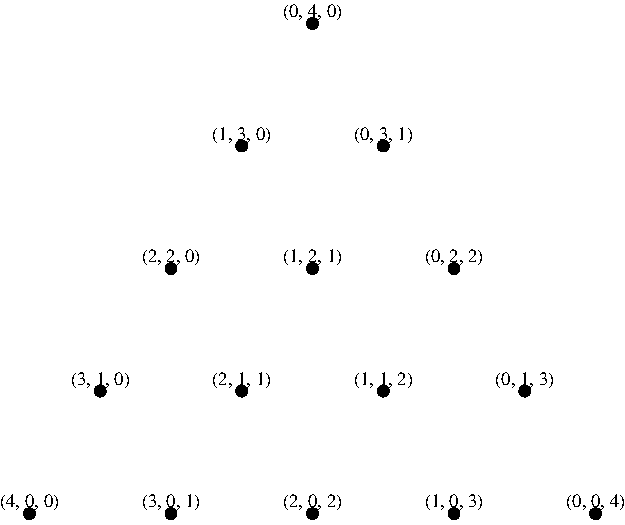
\includegraphics[width=0.45\textwidth]{figures/triangle_array_with_labels}
	\caption{Треугольный массив точек}
	\label{fig:triangle_array_with_labels}
\end{figure}
Взглянув на этот рисунок, можно легко подсчитать количество элементов в $\Delta_n$:
\[
	|\Delta_n| = 1 + 2 + \dotsb + n = \frac{n (n + 1)}{2}.
\]

Для $x \in \Delta_n$ будем писать $x = (x_1,x_2,x_3)$. Пусть $H_1, H_2, H_3$ подгруппы $S_{\Delta_n}$, которые сохраняют первую, вторую и третью координаты соответственно. А именно,
\[
	H_i = \{ \pi \in  S_{\Delta_n} \mid (\pi(x))_i = x_i \mbox{ для всех } x \in \Delta_n\}.
\]

\begin{theorem}\label{th:05:1.7}
  Подгруппы $H_1, H_2, H_3$, определённые выше, удовлетворяют свойству тройного произведения.
\end{theorem}
\begin{proof}
	Пусть $h_1h_2h_3=1$ с $h_i \in H_i$. Упорядочим тройки лексикографически так, что $(0,0,n-1)$ --- наименьшая тройка, а $(n-1,0,0)$ --- наибольшая, и докажем по индукции, что $h_1, h_2$ и $h_3$ фиксируют любую тройку.

	Предположим, что любая из перестановок $h_1, h_2$ и $h_3$ оставляет на месте все тройки меньше $(a,b,c)$ (в базовом случае множество таких троек пустое). Перестановка $h_3$ не может перевести  $(a,b,c)$  в меньшую тройку, так как все меньшие тройки зафиксированы, поэтому $h_3$ должна перевести её в $(a+i, b-i, c)$, где $i \geq 0$. Затем $h_2$ переводит её в $(a+i+j, b-i, c-j)$ для какого-то $j$.

	$h_1$ сможет вернуться к $(a,b,c)$ только если $i+j=0$, значит так оно и есть. Однако $h_1$ оставляет на месте $(a,b-i,c+i)$ для $i \geq 0$ (потому как такая тройка меньше чем $(a,b,c)$) поэтому $i=0$. Отсюда следует, что $(a,b,c)$ фиксируется каждым из $h_1, h_2, h_3$, поэтому по индукции все тройки зафиксированы, то есть $h_1=h_2=h_3=1$. 
\end{proof}

	\section{ОР-матрицы и усиленные ОР-матрицы}

\begin{definition}
  \textbf{Однозначно разрешимой матрицей} (сокр. ОР-матрицей, англ. uniquely solvable puzzle, USP) ширины $k$ называют подмножество $U \subseteq \left\{ 1,2,3 \right\}^k$, удовлетворяющее свойству: 
  
  для любой тройки перестановок $\pi_1, \pi_2, \pi_3 \in S_U$ либо $\pi_1=\pi_2=\pi_3$, либо существуют $u \in U$ и $i \in [k]$ такие, что по меньшей мере два равенства из 
  \[\left( \pi_1(u) \right)_i = 1,\; \left( \pi_2(u) \right)_i = 2,\; \left( \pi_3(u) \right)_i = 3\]
  выполняются. (Здесь $\left( \pi_j(u) \right)_i$ обозначает число, стоящее на $i$-ой позиции в строке $\pi_j(u)$.)
\end{definition}

В качестве примера ОР-матрицы ширины 6 и размера 8 можно привести следующую таблицу:
\begin{figure}[H]
	\begin{center}
	   \begin{tabular}{|c|c|c|c|c|c|}
	    \hline 
	    3 & 3 & 3 & 3 & 3 & 3\\ \hline
	    1 & 3 & 3 & 2 & 3 & 3\\ \hline
	    3 & 1 & 3 & 3 & 2 & 3\\ \hline
	    1 & 1 & 3 & 2 & 2 & 3\\ \hline
	    3 & 3 & 1 & 3 & 3 & 2\\ \hline
	    1 & 3 & 1 & 2 & 3 & 2\\ \hline
	    3 & 1 & 1 & 3 & 2 & 2\\ \hline
	    1 & 1 & 1 & 2 & 2 & 2\\ 
	    \hline
	  \end{tabular}
	\end{center}
	\caption{Пример ОР-матрицы}
	\label{usp}
\end{figure}
Замечу, что порядок, в котором следуют строки, значения не имеет. 

В английском наименовании этого объекта присутствует слово пазл, потому что ОР-матрицу можно рассматривать как своего рода головоломку. Пусть 
\[
u = \begin{array}{|c|c|c|c|c|c|} \hline 3 & 3 & 1 & 3 & 3 & 2 \\ \hline\end{array} 
\]
--- это один из элементов $U$. Он состоит из частей трёх типов
\[
	\begin{array}{|c|c|c|c|c|c|} \hline \; & \; & 1 & \; & \; & \;  \\ \hline\end{array}, 
	\begin{array}{|c|c|c|c|c|c|} \hline \; & \; & \;& \; & \; & 2 \\ \hline\end{array},
	\begin{array}{|c|c|c|c|c|c|} \hline 3 & 3 & \; & 3 & 3 & \; \\ \hline\end{array}.
\]
Чтобы собрать пазл, нужно переместить фрагменты первого, второго и третьего типов всех элементов $U$ в соответствии с перестановками $\pi_1, \pi_2, \pi_3$, и снова объединить их в таблицу так, чтобы в каждой строке новой матрицы были части каждого из трёх типов, и чтобы эти части не накладывались друг на друга. Определение требует, чтобы этот пазл имел единственное решение. То есть если среди перестановок $\pi_1, \pi_2, \pi_3$ будет по крайней мере две не равные между собой, то случится коллизия, то есть наложение частей. Если же все перестановки равны, то полученная в итоге матрица будет отличаться от исходной лишь порядком следования строк, что считается тем же самым решением.

Теперь немного подробнее. Сначала замечу, что для перестановок $\pi_1, \pi_2, \pi_3$ значение имеют только элементы 1,2 и 3 соответственно, стоящие в матрице. Поэтому лучше думать об этих перестановках не как о перемещающих строки целиком, а как о перемещающих фрагменты строк, содержащие их собственные числа. В этой интерпретации ОР-матрица с рисунка \ref{usp} будет выглядеть как:

\begin{figure}[H]
	\centering
    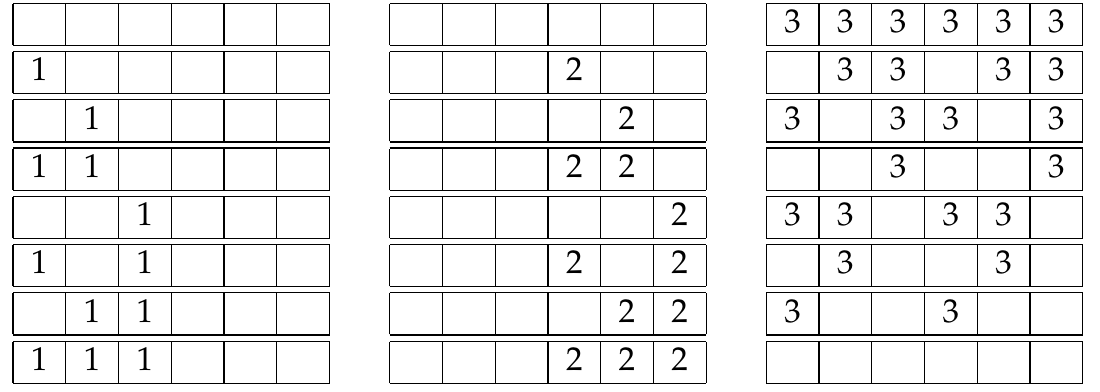
\includegraphics[width=0.5\textwidth]{figures/usp_pieces}
	\caption{фрагменты ОР-матрицы}
	\label{usp:fig3.2}
\end{figure}
Здесь в первую таблицу попадают все вхождения 1 в ОР-матрицу, во вторую --- 2, в третью --- 3. Далее $\pi_j$ перемещает строки таблицы, в которой стоят одни только $j$. В конце эти таблицы совмещаются. Равенство $(\pi_j(u))_i = j$ эквивалентно тому, что в итоговой таблице на пересечении строки $\pi_j(u)$ и столбца $i$ стоит число $j$. Поэтому из определения ОР-матрицы будет следовать, что если не все $\pi_j$ равны, то в итоговой таблице существует строка и столбец, на пересечении которых стоит больше одного элемента, то есть случилась коллизия, иначе говоря фрагменты пазла наложились друг на друга. 

Используя эту интерпретацию, докажем, что таблица с рисунка \ref{usp} на самом деле является ОР-матрицей. Без ограничения общности можно считать, что $\pi_3 = 1$ потому, что перебор всех троек $\pi_1, \pi_2, \pi_3$ эквивалентен перебору троек $\pi_1 \rho, \pi_2 \rho, \pi_3 \rho$ для какого-то $\rho \in S_U$. Выберем $\rho = \pi_3^{-1}$, в этом случае $\pi_1 \rho, \pi_2 \rho$ по-прежнему случайные перестановки, хотя $\pi_3 \rho$ теперь всегда равна 1. Это даст нам начальную позицию, изображённую ниже:
\begin{figure}[H]
	\centering
    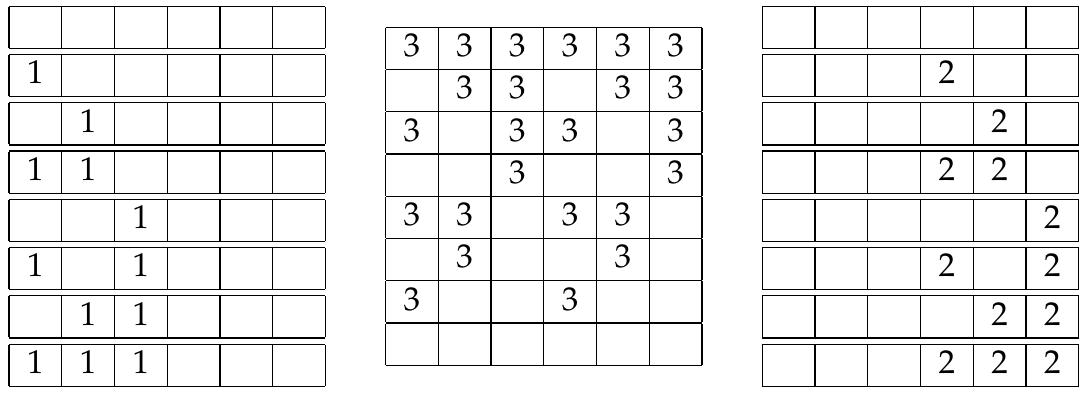
\includegraphics[width=0.5\textwidth]{figures/usp_threes_placed}
	\caption{фрагменты ОР-матрицы, где тройки уже на месте}
	\label{usp:fig3.3}
\end{figure}
Таблица в центре --- это пока ещё не завершённая итоговая таблица, оставшиеся части пазла изображены справа и слева. Так как $\pi_3 = 1$, мы знаем, что тройки уже стоят на своих местах.

Рассмотрим то, как будет выбираться место для фрагмента с тремя 1. Поскольку все строки, кроме последней, содержат 3 в одном из первых трёх столбцов, то попытка вставить этот фрагмент куда-либо помимо последней строки приведёт к коллизии. После того как фрагмент с тремя 1 займёт своё место пазл будет выглядеть так:
\begin{figure}[H]
	\centering
    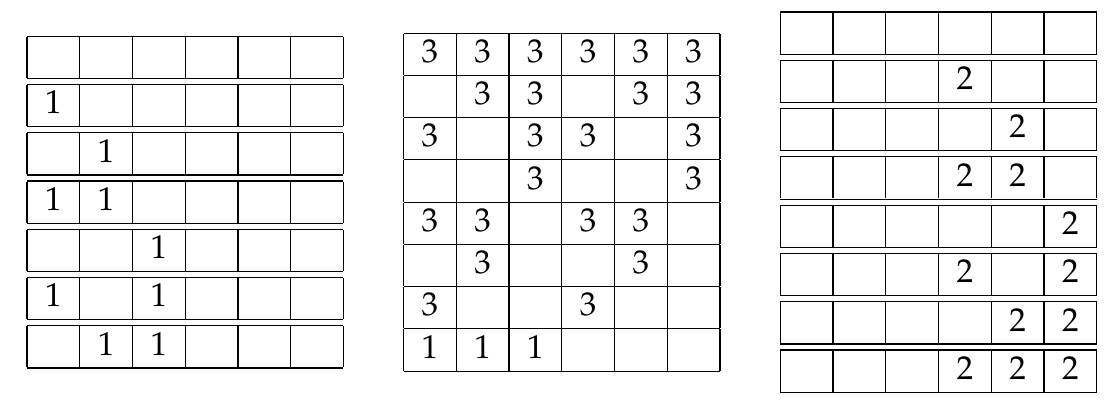
\includegraphics[width=0.5\textwidth]{figures/usp_threes_and_first_piece_placed}
	\caption{фрагменты ОР-матрицы, где тройки и фрагмент с тремя 1 уже на месте}
	\label{usp:fig3.4}
\end{figure}

Теперь рассматривая любой фрагмент с двумя 1, снова убеждаемся, что существует только одно место, куда его можно вставить без коллизий. Подобным же образом размещаются части с одной 1. В итоге получим:
\begin{figure}[H]
	\centering
    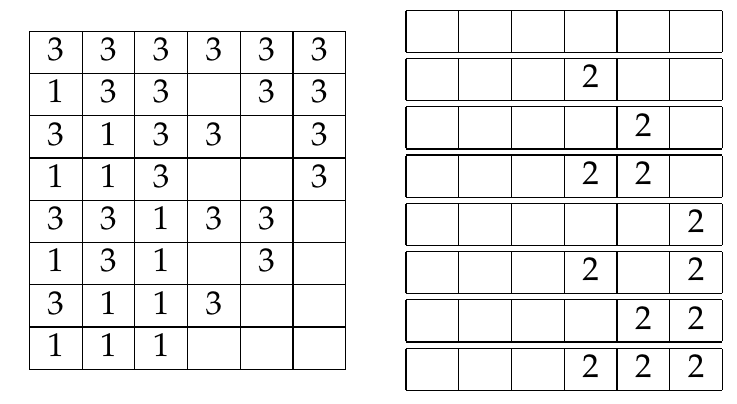
\includegraphics[width=0.5\textwidth]{figures/usp_threes_and_ones_placed.png}
	\caption{фрагменты ОР-матрицы, где тройки и единицы уже на месте}
	\label{usp:fig3.5}
\end{figure}

Так как структура фрагментов с двойками та же самая что и у фрагментов с единицами просто в других столбцах, ясно что они могут быть расположены единственным способом. Таким образом, показали, что матрица с рисунка \ref{usp} имеет единственное решение и поэтому на самом деле будет ОР-матрицей.

Нужно сделать одно дополнительное замечание о том случае, когда у таблицы, претендующей на звание ОР-матрицы, два фрагмента или строки идентичны, то есть имеют одни и те же числа и конфигурацию. В этом случае можно взять перестановку, которая будет просто менять эти две строки местами, что не будет менять саму матрицу, а две другие перестановки взять тривиальными. Тогда итоговая таблица будет идентична изначальной, то есть коллизий не будет, но также не будет выполняться условие $\pi_1=\pi_2=\pi_3$. Поэтому такая матрица не может быть однозначно разрешимой. Эта ситуация похожа на ту, когда в пазле есть два совершенно неотличимых фрагмента, и, конечно же, такой пазл не будет иметь единственного решения.

\begin{definition}
  \textbf{Усиленной ОР-матрицей} (сокр. УОР-матрицей) называют ОР-матрицу, у которой определяющее свойство было усилено следующим образом:
  
  для любой тройки перестановок $\pi_1, \pi_2, \pi_3 \in S_U$ либо $\pi_1=\pi_2=\pi_3$, либо существуют $u \in U$ и $i \in [k]$ такие, что \textbf{в точности} два равенства из 
  \[\left( \pi_1(u) \right)_i = 1,\; \left( \pi_2(u) \right)_i = 2,\; \left( \pi_3(u) \right)_i = 3\]
  выполняются.
\end{definition}

Возвращаясь к аналогии с пазлом, это условие означает, что теперь если в каких-то позициях произойдёт одновременное наложение сразу трёх фрагментов, это не будет нарушением правил сборки головоломки, то есть гораздо меньше матриц будет иметь единственное решение, поэтому это условие будет сильнее чем исходное.

Нетрудно заметить, что матрица с рисунка \ref{usp} будет УОР-матрицей, поскольку в каждом её столбце встречаются только два из возможных трёх символов $\left\{ 1,2,3 \right\}$. Эту конструкцию можно обобщить.

\begin{prop}\label{prop:05:3.1}
  Для любого $k \geq 1$ существует УОР-матрица размера $2^k$ и ширины $2k$.
\end{prop}
\begin{proof}
	Если смотреть на $\left\{ 1,3 \right\}^k \times \left\{ 2,3 \right\}^k$ как на подмножество $\left\{ 1,2,3 \right\}^{2k}$, определим $U$ следующим образом:
	\[
		\left\{ u \in \left\{ 1,3 \right\}^k \times \left\{ 2,3 \right\}^k | \text{ для } i \in [k], \; u_i = 1 \iff u_{i+k} = 2 \right\}.
	\]
	Пусть $\pi_1, \pi_2, \pi_3 \in S_U$. Если $\pi_1 \neq \pi_3$, тогда существует $u \in U$ такой, что $\left( \pi_1(u) \right)_i = 1$ и $\left( \pi_3(u) \right)_i = 3$ для
	какого-то $i \in [k]$. Точно также, если $\pi_2 \neq \pi_3$, тогда существует $u \in U$ такой, что $\left( \pi_2(u) \right)_i = 2$ и $\left( \pi_3(u) \right)_i = 3$ для
	какого-то $i \in [2k]\setminus[k]$. В любом случае в точности два равенства из $\left( \pi_1(u) \right)_i = 1,\; \left( \pi_2(u) \right)_i = 2,\; \left( \pi_3(u) \right)_i = 3$ выполняются, потому что в каждой координате могут встретиться только два из трёх символов $\left\{ 1,2,3 \right\}$. Отсюда следует, что $U$ является УОР-матрицей. 
\end{proof}

\begin{definition}
  \textbf{УОР-ёмкостью} называют наибольшую константу $C$ такую, что существуют УОР-матрицы размера $(C - o(1))^k$ и ширины $k$ для бесконечного количества значений $k$. \textbf{ОР-ёмкость} определяется аналогично.
\end{definition}

Существует простая верхняя оценка для ОР-ёмкости, которая, конечно, также будет верхней оценкой для УОР-ёмкости:
\begin{lemma} \label{lem:05:3.2}
  ОР-ёмкость не превышает ${3 \over 2^{2 / 3}}$.
\end{lemma}
\begin{proof}
  Пусть $U$ --- ОР-матрица ширины $k$. Для каждой тройки $n_1, \; n_2, \; n_3$ неотрицательных целых чисел, дающих в сумме $k$, определим $U_{u_1,u_2,u_3}$ как подмножество элементов $U$, которые имеют $n_1$ позицию с 1, $n_2$ позиций с 2, и $n_3$ с 3. Существует всего $\binom{k+2}{2}$ способов выбрать $n_1, n_2$ и $n_3$ поэтому
  \[
  	|U| \leq \dbinom{k+2}{2} \max_{n_1,n_2,n_3} |U_{n_1,n_2,n_3}|.
  \]
  Если два элемента $U$ имеют 1 в одних и тех же позициях, то если взять в качестве $\pi_1$ перестановку, которая меняет местами эти элементы, а $\pi_2, \pi_3$ взять тривиальными, то получим противоречие с определением ОР-матрицы, поэтому $|U_{n_1,n_2,n_3}|$ не может превосходить число способов, которым можно распределить $n_1$ единицу по имеющимся $k$ позициям, конечно, тоже самое будет верно для 2 и 3. Таким образом,
  \[
  	|U_{n_1,n_2,n_3}| \leq \min_i \dbinom{k}{n_i} \leq \left( {3 \over 2^{2/3}} + o(1)\right)^k,
  \]
  где последнее неравенство выполняется потому, что $\min_i \binom{k}{n_i}$ максимально, когда $n_1=n_2=n_3=k/3$. 
  
  \begin{align*}
    \ln \dbinom{k}{k/3} & = \ln \frac{k!}{(\frac{2k}{3})!(\frac{k}{3})!}\\
    & = \ln k! - \ln \left( \frac{2k}{3} \right)! - \ln \left( \frac{k}{3} \right)! \\
    & = k \ln k - \cancel{k} - \frac{2k}{3} \ln \frac{2k}{3} + \cancel{\frac{2k}{3}} - \frac{k}{3} \ln \frac{k}{3} + \cancel{\frac{k}{3}} + O(\ln k) \text{ (по формуле Стирлинга) }\\
    & = k \left( \ln k - \frac{2}{3} \ln \frac{2k}{3} - \frac{1}{3} \ln \frac{k}{3} \right) + O(\ln k)\\
    & = k \left( \cancel{\ln k} - \cancel{\frac{2}{3} \ln k} - \frac{2}{3} \ln \frac{2}{3} - \cancel{\frac{1}{3} \ln k} - \frac{1}{3} \ln \frac{1}{3} \right) + O(\ln k) \\
    & = k \left( - \frac{2}{3} \ln 2 + \frac{2}{3} \ln 3 + \frac{1}{3} \ln 3 \right) + O(\ln k)\\
    & = k \ln \frac{3}{2^{2/3}} + O(\ln k)\\
    & = k \left( \ln \left( \frac{3}{2^{2/3}} + o(1) \right) \right)
  \end{align*}
  \begin{question}
    Правильно ли я внёс $O(\ln k) / k$ в логарифм с получением в итоге $o(1)$?
  \end{question}
  Отсюда следует, что $|U| \leq \left( {3 \over 2^{2/3}} + o(1)\right)^k$, что и требовалось доказать.
\end{proof}

ОР-матрицы неявно присутствуют в статье Копперсмита и Винограда \cite{Coppersmith:1990}. Раздел 6 их статьи можно интерпретировать как вероятностную конструкцию, показывающую, что лемма \ref{lem:05:3.2} точная.

\begin{theorem} (Копперсмит и Виноград \cite{Coppersmith:1990}) \label{th:05:3.3}
  ОР-ёмкость равна ${3 \over 2^{2 / 3}}$.
\end{theorem}

Кон и др. в статье \cite{Cohn05} выдвинули гипотезу, что тоже будет верно для УОР-ёмкости. Если их гипотеза верна, то это будет означать, что $\omega=2$.
\begin{conj} \label{conj:05:3.4}
  УОР-ёмкость равна ${3 \over 2^{2 / 3}}$.
\end{conj}















	\section{Подсолнечники}

Существуют следствия из различных открытых проблем, которые говорят, что гипотеза \ref{conj:05:3.4} скорее всего неверна, то есть УОР-ёмкость не достигает ${3 \over 2^{2 / 3}}$.
Эти следствия рассматриваются в статье Алона и др. \cite{Alon11} и касаются комбинаторного объекта, называемого подсолнечником.

\begin{definition}
  \textbf{$k$-подсолнечник} --- это коллекция $k$ подмножеств $S_1, \dotsc, S_k$, имеющих одинаковые попарные пересечения. То есть для любого $x \in \bigcup_{i=1}^k S_i$ либо $x$ находится в одном множестве, либо во всех $k$ подмножествах.
\end{definition}

Наиболее интересным вопросом, связанным с подсолнечниками будет следующий: дано семейство $\mathcal{F}$, на сколько большим должно быть семейство чтобы в нём содержался подсолнечник. Эту задачу поставили Эрдёш и Радо в статье 1960 года. В ней они доказали следующую фундаментальную теорему о подсолнечниках:
\begin{theorem}
  Пусть $\mathcal{F}$ --- семейство множеств, каждое с мощностью $s$. Если $|\mathcal{F}| > (k-1)^s s!$, тогда $\mathcal{F}$ содержит $k$-подсолнечник.
\end{theorem}
В той же статье была выдвинута гипотеза, являющаяся одной из самых изучаемых в комбинаторике
\begin{conj}
  Пусть $\mathcal{F}$ --- семейство множеств, каждое с мощностью $s$. Существует константа $c_k$, зависящая только от $k$ такая, что если $|\mathcal{F}| \geq c_k^s$, то $\mathcal{F}$ содержит $k$-подсолнечник.
\end{conj}

Хотя эта гипотеза не связана напрямую с УОР-матрицами, Алон и др. \cite{Alon11} представили серию очень сложных её обобщений, чтобы описать которые потребовалось бы привести всю их статью, поэтому заинтересованным читателям следует обратиться к первоисточнику.

	\section{Использование УОР-матриц}

Дана УОР-матрица $U$ ширины $k$, пусть $H$ --- абелева группа всех функций из $U \times [k]$ в циклическую группу $Cyc_m$ ($H$ является группой относительно поточечного сложения). Симметрическая группа $S_U$ действует на $H$ следующим образом:
\[
	\pi(h)(u,i)=h(\pi^{-1}(u),i)
\]
для $\pi \in S_U, \; h \in H, \; u \in U$ и $i \in [k]$. Интуитивно можно смотреть на элементы из $H$ как на таблицы того же размера что и $U$. Отличие в том, что в таблицах, соответствующих элементам из $H$, стоят элементы из $Cyc_m$, а не числа из $\left\{ 1,2,3 \right\}$. Эти таблицы можно складывать по правилам сложения обычных матриц. Действие $\pi \in S_U$ на $h \in H$ будет переставлять строки в соответствующей таблице.

Пусть $G$ --- полупрямое произведение $H \rtimes S_U$, определим подмножества $S_1, S_2, S_3$ так: $S_i$ состоит из всех произведений $h \pi$, где $\pi \in S_U$, и элемент $h \in H$ удовлетворяет условию:
\[
	h(u,j) \neq 0 \iff u_j=i
\]
для всех $u \in U$ и $j \in [k]$. Возвращаясь к аналогии с таблицами, у таблицы $h$ в данной позиции стоит ненулевой элемент тогда и только тогда, когда в соответствующей позиции  УОР-матрицы $U$ стоит $i$. На перестановку $\pi$ ограничения не налагаются.
\begin{figure}[H]
	\centering
    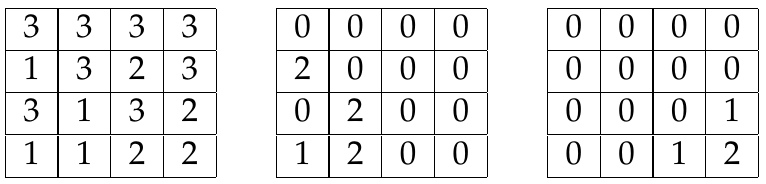
\includegraphics[width=0.5\textwidth]{figures/small_usp_and_group_elements}
	\caption{небольшая УОР-матрица и элементы группы $H$}
	\label{usp:fig3.6}
\end{figure}

На рисунке \ref{usp:fig3.6} показан пример небольшой УОР-матрицы $U$, справа от которой пара элементов из $H$, где $m=3$, и поэтому в них стоят числа из $\left\{ 0,1,2 \right\}$. Здесь элемент, стоящий в центре, будет содержаться в $S_1$, тогда как элемент справа не входит ни в одно из множеств $S_i$.

\begin{prop}\label{prop:05:3.5}
  Если $U$ --- УОР-матрица, то $S_1, S_2, S_3$ удовлетворяют свойству тройного произведения.
\end{prop}
\begin{proof}
  Рассмотрим тройное произведение
  \begin{equation} \label{eq:3.1}
  	h_1 \pi_1 \pi_1'^{-1} h_1'^{-1} h_2 \pi_2 \pi_2'^{-1} h_2'^{-1} h_3 \pi_3 \pi_3'^{-1} h_3'^{-1} = 1, \text{ где } h_i \pi_i, h_i' \pi_i' \in S_i.
  \end{equation}
  
  Если привести это уравнение по всем правилам, действующим в полупрямых произведениях, получим
  \[
  	(h_1 + \pi_1 \pi_1'^{-1} \cdot (h_1'^{-1}h_2) + \pi_1 \pi_1'^{-1} \pi_2 \pi_2'^{-1} \cdot (h_2'^{-1}h_3) + \pi_1 \pi_1'^{-1} \pi_2 \pi_2'^{-1} \pi_3 \pi_3'^{-1} \cdot h_3'^{-1}) \pi_1 \pi_1'^{-1} \pi_2 \pi_2'^{-1} \pi_3 \pi_3'^{-1} = 1,
  \]
  где всё, что стоит в скобках является элементом из $H$, <<$\cdot$>> как обычно обозначает действие. Стоит заметить, что так как $H$ абелева, то операция в ней будет иметь аддитивную форму, то есть все $h_i'^{-1}$ впоследствии будут преобразованы в $-h_i'$.
  
  Чтобы \eqref{eq:3.1} выполнялось должно быть 
  \begin{equation} \label{eq:3.2}
  	\pi_1 \pi_1'^{-1} \pi_2 \pi_2'^{-1} \pi_3 \pi_3'^{-1} = 1.
  \end{equation}
  Зададим $\pi = \pi_1 \pi_1'^{-1}$ и $\rho = \pi_1 \pi_1'^{-1} \pi_2 \pi_2'^{-1}$. Тогда для того, чтобы \eqref{eq:3.1} было верно в группе $H$ должно выполняться условие:
  \begin{equation} \label{eq:3.3}
  	h_1 - h_3' + \pi (h_2 - h_1') + \rho (h_3 - h_2') = 0.
  \end{equation}
  
  Обратите внимание, что
  \begin{align*}
  	(h_1 - h_3')(u,j) & \neq 0  \iff  u_j \in \left\{ 1,3 \right\}\\
  	\pi(h_2 - h_1')(u,j) & \neq 0 \iff  (\pi^{-1}(u))_j \in \left\{ 2,1 \right\}\\
  	\rho(h_3 - h_2')(u,j) & \neq 0 \iff  (\rho^{-1}(u))_j \in \left\{ 3,2 \right\}.
  \end{align*}
  
  По определению УОР-матрицы либо $\pi=\rho=1$, либо существуют $u$ и $j$ такие, что в точности одно из этих трёх условий выполняется, но в этом случае \eqref{eq:3.3} не может быть верным.
  
  Теперь тоже самое, но подробнее. Рассмотрим следующую тройку перестановок $\rho^{-1}, 1, \pi^{-1} \in S_U$, из определения УОР-матрицы получим, что либо $\rho^{-1}= 1= \pi^{-1}$ либо $\exists u \in U, j \in [k]$ такие, что в точности 2 из 3 равенств $(\rho^{-1}(u))_j=1, u_j=2, (\pi^{-1}(u))_j=3$ верны. Пусть не выполняется первое равенство, тогда:
  \begin{align*}
  		(\rho^{-1}(u))_j \in \left\{ 2,3 \right\} & \implies \rho(h_3-h_2')(u,j) \neq 0\\
  		u_j = 2 & \implies (h_1 - h_3')(u,j) = 0\\
  		(\pi^{-1}(u))_j=3 & \implies \pi(h_2 - h_1')(u,j) = 0.
  \end{align*}
  
  Откуда следует, что \eqref{eq:3.3} не может выполняться, так как одно из слагаемых не равно нулю. Аналогично рассматриваются случаи, когда $u_j \neq 2$ и $(\pi^{-1}(u))_j \neq 3$.
  
  Таким образом, $\pi=\rho=1$, что вместе с \eqref{eq:3.2} означает $\pi_i = \pi_i'$ для всех $i$. Тогда имеем $h_1+h_2+h_3=h_1'+h_2'+h_3'$, откуда получаем $h_i'=h_i$ для всех $i$ потому, что только у $h_i$ и $h_i'$ в таблицах ненулевые элементы стоят в одних и тех же позициях. В итоге свойство тройного произведения выполняется.
\end{proof}

\begin{corollary}\label{cor:05:3.6}
  Если $U$ --- УОР-матрица ширины $k$ и $m \geq 3$, тогда 
  \[
  	\omega \leq \frac{3 \ln m}{\ln(m-1)} - \frac{3 \ln |U|!}{|U| k \ln(m-1)}
  \]
  В частности, если УОР-ёмкость равна $C$, тогда
  \[
  	\omega \leq \frac{3(\ln m - \ln C)}{\ln(m-1)}.
  \]
\end{corollary}
\begin{proof}
  Если $G$ реализует $\left\langle |S_1|,|S_2|,|S_3| \right\rangle$, то из следствия \ref{cor:05:1.9} и того, что $|G:H|=|U|!$ является наибольшей степенью неприводимого характера $G$, получим
  \begin{equation}\label{eq:s}
  	(|S_1||S_2||S_3|)^{\omega/3} \leq (|U|!)^{\omega-2}|G|.
  \end{equation}
  Мощность множества
  \[
  	|S_i|=(m-1)^{\text{количество $i$ в $U$}}\cdot |U|!.
  \]
  Итого
  \[
  	|S_1||S_2||S_3| = (m-1)^{|U|k}(|U|!)^3.
  \]
  Отмечу, что $|H|=m^{|U|k}$. Следовательно $|G|=m^{|U|k}|U|!$. Подставив в \eqref{eq:s} посчитанные значения получим:
  \begin{align*}
  	((m-1)^{|U|k}(|U|!)^3)^{\omega/3} & \leq (|U|!)^{\omega-2}m^{|U|k}|U|!\\
  	(m-1)^{\frac{|U|k}{3} \omega} (|U|!)^\omega & \leq \frac{m^{|U|k}}{|U|!}(|U|!)^\omega\\
  	\omega \frac{|U|k}{3} \ln (m-1) & \leq \ln \frac{m^{|U|k}}{|U|!}\\
  	\omega & \leq 3 \frac{|U|k \ln m - \ln |U|!}{|U|k \ln(m-1)} = \frac{3 \ln m}{\ln (m-1)} - \frac{3 \ln |U|!}{|U|k \ln(m-1)}.
  \end{align*}
  Из формулы Стирлинга легко получить, что
  \[
  	\ln n! = \ln \frac{n^n}{e^n} \sqrt{2 \pi n} (1 + o(1)) = n \ln n (1 + o(1)).
  \]
  \begin{question}
    Как выводятся друг из друга различные формы формулы Стирлинга?
    \begin{align*}
      \ln n! & = n \ln n - n + O(\ln(n))\\
      \ln n! & = n \ln n (1 + o(1)) \overset{?}{=} n \ln (n (1 + o(1)))
    \end{align*}
  \end{question}
  По определению УОР-ёмкости $C$ найдутся такие $U$, что $|U|=(C - o(1))^k$.
  \[
  	\frac{3 \ln |U|!}{|U|k \ln(m-1)} = \frac{3 \cancel{|U|} \ln |U| (1+o(1))}{\cancel{|U|}k \ln (m-1)} = \frac{3 \cancel{k} \ln (C - o(1))}{\cancel{k} \ln (m-1)}.
  \]
  \begin{question}
    Правильно ли я здесь обращаюсь с $o(1)$?
  \end{question}
  В итоге
  \[
  	\omega \leq \frac{3 \ln m}{\ln (m-1)} - \frac{3 \ln C}{\ln (m-1)} = \frac{3 (\ln m - \ln C)}{\ln (m-1)}. \qedhere
  \]
\end{proof}

С помощью утверждения \ref{prop:05:3.1} можно получить оценку $\omega < 2.67$ при $m=9$. В следующем разделе будет показано, что УОР-ёмкость по меньшей мере равна $2^{2/3}$, и поэтому $\omega < 2.48$, что является наилучшей известной оценкой, полученной при помощи УОР-матриц.

Если гипотеза \ref{conj:05:3.4} верна, то следствие \ref{cor:05:3.6} даст оценку $\omega = 2$ при $m=3$.




	\section{Треугольная конструкция}\label{triangle_construction}

У УОР-матриц, построенных в утверждении \ref{prop:05:3.1}, было свойство: каждый столбец содержал только два символа из возможных трёх $\left\{ 1,2,3 \right\}$. Любая ОР-матрица, обладающая этим свойством, будет также УОР-матрицей. Ниже будет рассмотрен вопрос насколько большими могут быть матрицы такого вида.

Пусть $U \subseteq \left\{ 1,2,3 \right\}^k$ --- матрица, у которой каждый столбец содержит только два символа. Через $U_{1,2}$ обозначим подматрицу $U$, образованную всеми столбцами, содержащими только символы 1 и 2. Аналогично определим матрицы $U_{2,3}$ и $U_{1,3}$. Без ограничения общности можно считать, что $U$ получается в результате объединения матриц $U_{1,2}, U_{2,3}$ и $U_{1,3}$, поэтому
\[
	U = ||U_{1,2} U_{2,3} U_{1,3}||.
\]

Через $H_1$ обозначим подгруппу $S_U$, сохраняющую столбцы $U$, содержащие только 1 и 2. Иными словами $H_1$ образована всеми перестановками $\pi$, обладающими свойством:\\
\textit{для любой строки $u \in U$ строка $\pi(u)$ совпадает с $u$ во всех координатах, соответствующим столбцам, содержащим только 1 и 2 (таким образом, если $U = ||U_{1,2} U_{2,3} U_{1,3}||$, то $\pi(U) = ||U_{1,2} \widetilde{U}_{2,3} \widetilde{U}_{1,3}||$).}

Аналогично $H_2$ сохраняет столбцы, содержащие только 2 и 3, а $H_3$ --- 1 и 3.

\begin{lemma}\label{lem:05:3.7}
  Множество $U$ является ОР-матрицей тогда и только тогда, когда $H_1,H_2$ и $H_3$ удовлетворяют свойству тройного произведения внутри $S_U$.
\end{lemma}
\begin{proof}
Пусть $\pi_1, \pi_2, \pi_3 \in S_U$. Перестановка $\pi_1 \pi_2^{-1}$ не содержится в $H_1$ тогда и только тогда, когда существует $v \in U$ и координата $i$ такие, что $v_i = 2$ и $((\pi_1 \pi_2^{-1})(v))_i=1$. Если положим $u=\pi_2^{-1}(v)$, то это эквивалентно тому, что $(\pi_2(u))_i=2$ и $(\pi_1(u))_i=1$. Аналогично выводятся условия для $\pi_2 \pi_3^{-1}$ и $\pi_3 \pi_1^{-1}$. Формально все три условия выглядят следующим образом:
\begin{align}
	\label{eq:tc1}
	\pi_1 \pi_2^{-1} \notin H_1  \iff \exists u, i :  (\pi_1(u))_i=1 \text{ и } (\pi_2(u))_i=2\\
	\label{eq:tc2}
	\pi_2 \pi_3^{-1} \notin H_2  \iff \exists u, i :  (\pi_2(u))_i=2 \text{ и } (\pi_3(u))_i=3\\
	\label{eq:tc3}
	\pi_3 \pi_1^{-1} \notin H_3  \iff \exists u, i :  (\pi_3(u))_i=3 \text{ и } (\pi_1(u))_i=1
\end{align}

\begin{question}
  Верны ли мои доказательства, представленные ниже?
\end{question}
$(\Longrightarrow)$ Пусть $U$ --- ОР-матрица, у которой каждый столбец содержит только два символа, докажем, что тогда $H_1, H_2, H_3$ удовлетворяют свойству тройного произведения в $S_U$.
Пусть $h_i \in H_i$ такие, что 
\[
	h_1 h_2 h_3 = 1.
\]
Любые элементы, удовлетворяющие этому равенству, можно записать в виде $h_1 = \pi_1 \pi_2^{-1}, h_2 = \pi_2 \pi_3^{-1}$ и $h_3 = \pi_3 \pi_1^{-1}$. Раз $U$ является ОР-матрицей, то для любых $\pi_1, \pi_2, \pi_3$ верно, что либо $\pi_1= \pi_2= \pi_3$, откуда $h_1=h_2=h_3=1$, либо существуют $u \in U, i \in [k]$ такие, что по крайней мере два равенства из $(\pi_1(u))_i=1, (\pi_2(u))_i=2, (\pi_3(u))_i=3$ выполняются, откуда получим противоречие, так как выходит, что для какого-то $j$ $h_j \notin H_j$. Подробнее, скажем, пусть верны $(\pi_1(u))_i=1$ и $(\pi_2(u))_i=2$, отсюда из \eqref{eq:tc1} будет следовать, что $\pi_1 \pi_2^{-1} = h_1 \notin H_1$.

$(\Longleftarrow)$ $H_1,H_2,H_3$ удовлетворяют свойству тройного произведения. Докажем, что $U$ --- ОР-матрица. Предположим противное, $U$ не является ОР-матрицей. Из этого будет следовать, что существуют перестановки $\pi_1, \pi_2, \pi_3 \in S_U$, хотя бы две из которых не равны и такие, что только 1 из равенств $(\pi_1(u))_i=1, (\pi_2(u))_i=2, (\pi_3(u))_i=3$ выполняется для всех $u \in U$ и всех $i \in [k]$. Из условий \eqref{eq:tc1}, \eqref{eq:tc2}, \eqref{eq:tc3} следует, что в этом случае $\pi_1 \pi_2^{-1} =: h_1 \in H_1, \pi_2 \pi_3^{-1} =: h_2 \in H_2$ и $\pi_3 \pi_1^{-1} =: h_3 \in H_3$. Исходя из задания элементов $h_1, h_2, h_3$ получим, что $h_1 h_2 h_3 = 1$, и так как $H_1, H_2$ и $H_3$ удовлетворяют свойству тройного произведения имеем, что $h_1=h_2=h_3=1$, следовательно $\pi_1= \pi_2= \pi_3$ --- противоречие с тем, что хотя бы две перестановки из $\pi_1, \pi_2, \pi_3$ не равны между собой. 
\end{proof}

\begin{prop}\label{prop:05:3.8}
  Для любого $k \geq 1$ существует УОР-матрица размера ${2^{k-1}(2^k + 1)}$ и ширины $3k$.
  
  Из этого будет следовать, что УОР-ёмкость не меньше, чем $2^{2/3}$ и $\omega < 2.48$.
\end{prop}
\begin{proof}
Рассмотрим треугольник
\[
	\Delta_n = \left\{ (a,b,c) \in \mathbb{Z}^3 \mid a+b+c=n-1 \text{ и } a,b,c \geq 0\right\},
\]
где $n=2^k$, и пусть $H_1, H_2$ и $H_3$ являются подгруппами $S_{\Delta_n}$, сохраняющими первую, вторую и третью координаты у элементов $(a,b,c)$ соответственно. По теореме \ref{th:05:1.7} эти подгруппы удовлетворяют свойству тройного произведения в $S_{\Delta_n}$.

Чтобы построить требуемую УОР-матрицу, выберем подмножество $U \subseteq \left\{ 1,2,3 \right\}^{3k}$ следующим образом. В первых $k$ координатах будут встречаться только 1 и 2, во вторых $k$ координатах только 2 и 3, в третьих --- только 1 и 3. В каждом из этих блоков по $k$ координат существует $2^k$ возможных способов расставить два доступных символа. Пронумеруем эти способы числами от 0 до $2^k-1$ (причём номер получает сам способ чередования двух символов, то есть, какие именно символы чередуются, значения не имеет. Например, при $k=3$ блоки $\begin{array}{|c|c|c|} \hline 2 & 1 & 1 \\ \hline\end{array}, \; \begin{array}{|c|c|c|} \hline 3 & 2 & 2 \\ \hline\end{array}$ и $\begin{array}{|c|c|c|} \hline 3 & 1 & 1 \\ \hline\end{array}$ имеют один и тот же номер.) Элементы из $U$ будут соответствовать элементам из $\Delta_n$ следующим образом: $u \in U$ соответствует $(a,b,c) \in \Delta_n$, если в первых $k$ координатах 2 символа чередуются способом под номером $a$, во вторых --- способом $b$, а в третьих --- способом $c$. Из леммы \ref{lem:05:3.7} следует, что $U$ будет УОР-матрицей. Всего существует $n(n+1)/2$ троек $(a,b,c)$, где $a,b,c \geq 0$ и $a + b + c = n-1$, поэтому  
\[
	|U|=|\Delta_n| = \frac{n(n+1)}{2} = \frac{2^k (2^k + 1)}{2} = 2^{k-1}(2^k + 1).\qedhere
\]
\end{proof}

Можно показать, используя лемму \ref{lem:05:3.7}, что это построение оптимально:
\begin{corollary}
  Если $U$ --- ОР-матрица ширины $k$ такая, что только 2 символа встречаются в каждой координате, то $|U| \leq (2^{2/3} + o(1))^k$.
\end{corollary}

Условие о том, что в каждой координате встречаются только 2 из 3 символов сильно ограничивает выбор, но улучшить утверждение \ref{prop:05:3.8} пока не удалось. Однако также не известно верхних оценок на размер УОР-матриц кроме леммы \ref{lem:05:3.2}. 






































	\section{Свойство совместного двойного произведения}

Существует по меньшей мере два естественных направления для улучшения конструкции из раздела \ref{triangle_construction}. В комбинаторном направлении можно надеяться заменить УОР-матрицу из утверждения \ref{prop:05:3.8} на большую, что позволит достичь экспоненты 2, если гипотеза \ref{conj:05:3.4} верна. В алгебраическом направлении, можно оставить комбинаторную треугольную конструкцию на месте, а вместо этого модифицировать лежащую в основе группу. Такая модификация может быть произведена при помощи свойства совместного двойного произведения, которое приведено ниже, и есть основания полагать, что этим способом также можно достичь $\omega=2$ (гипотеза \ref{conj:05:4.7}).

\begin{definition}
 Будем говорить, что подмножества $S_1, S_2$ группы $H$ удовлетворяют \textbf{свойству двойного произведения} (англ. double product property), если
 \[
 	q_1 q_2 = 1 \implies q_1 = q_2 = 1,
 \]  
 где $q_i \in Q(S_i)$.
\end{definition}

\begin{definition}\label{def:05:4.1}
  Будем говорить, что $n$ пар подмножеств $A_i, B_i$ (для $1 \leq i \leq n$) группы $H$ удовлетворяют \textbf{свойству совместного двойного произведения} (англ. simultaneous double product property), если
  \begin{itemize}
    \item для всех $i$ пары $A_i, B_i$ удовлетворяют свойству двойного произведения и 
    \item для всех $i,j,k$ 
    \[
    	a_i (a_j')^{-1} b_j (b_k')^{-1} = 1 \text{ означает } i=k,
    \]
    где $a_i \in A_i, a_j' \in A_j, b_j \in B_j, b_k' \in B_k$.
  \end{itemize}
\end{definition}

Можно переформулировать последнее условие так: 

\textit{если рассматривать множества
\[
	A_i^{-1} B_j = \left\{ a^{-1}b \mid a \in A_i, b \in B_j \right\}
\]
те из них, у которых $i=j$, не пересекаются с теми, у которых $i \neq j$.}

Тривиальным примером будет $H = Cyc_n^k \times Cyc_n$ и множества $A_i = \left\{ (x,i) \mid x \in Cyc_n^k \right\}$ и $B_i = \left\{ (0,i) \right\}$. Тогда пары $A_i, B_i$ для $i \in Cyc_n$ удовлетворяют свойству совместного двойного произведения.

\begin{lemma}\label{lem:05:4.2}
  Если $n$ пар подмножеств $A_i, B_i \subseteq H$ удовлетворяют свойству совместного двойного произведения, и $n'$ пар подмножеств $A_i', B_i' \subseteq H'$ удовлетворяют свойству совместного двойного произведения, тогда $n n'$ пар $A_i \times A_j', B_i \times B_j' \subseteq H \times H'$ также будут ему удовлетворять.
\end{lemma}

Пары $A_i, B_i$, удовлетворяющие свойству совместного двойного произведения в группе $H$, могут быть преобразованы в подмножества, удовлетворяющие свойству тройного произведения. Напомню, что
\[
	\Delta_n = \left\{ (a,b,c) \in \mathbb{Z}^3 \mid a+b+c=n-1 \text{ и } a,b,c \geq 0\right\}.
\]

Пусть дано $n$ пар подмножеств $A_i, B_i$ в $H$  для $0 \leq i \leq n-1$, определим тройки подмножеств в $H^3$ с индексами $v=(v_1,v_2,v_3) \in \Delta_n$ следующим образом:
\begin{align*}
  \widehat{A}_v & = A_{v_1} \times \left\{ 1 \right\} \times B_{v_3}\\
  \widehat{B}_v & = B_{v_1} \times A_{v_2} \times \left\{ 1 \right\}\\
  \widehat{C}_v & = \left\{ 1 \right\} \times B_{v_2} \times A_{v_3}
\end{align*}

\begin{theorem}\label{th:05:4.3}
  Если $n$ пар подмножеств $A_i, B_i \subseteq H$ (с $0 \leq i \leq n-1$) удовлетворяют свойству совместного двойного произведения, то следующие подмножества $S_1,S_2,S_3$ группы $G=(H^3)^{|\Delta_n|} \rtimes S_{\Delta_n} $ удовлетворяют свойству тройного произведения:
  \begin{align*}
    S_1 & = \left\{ \widehat{a} \pi \mid \pi \in S_{\Delta_n},  \widehat{a}_v \in \widehat{A}_v \text{ для всех } v \right\}\\
    S_2 & = \left\{ \widehat{b} \pi \mid \pi \in S_{\Delta_n},  \widehat{b}_v \in \widehat{B}_v \text{ для всех } v \right\}\\
    S_3 & = \left\{ \widehat{c} \pi \mid \pi \in S_{\Delta_n},  \widehat{c}_v \in \widehat{C}_v \text{ для всех } v \right\}
  \end{align*}
\end{theorem}

Увы, авторы статьи не привели доказательства этой теоремы, известно лишь, что в нём используется теорема \ref{th:05:1.7}, и оно подобно доказательству утверждения \ref{prop:05:3.5}.

\begin{theorem}\label{th:05:4.4}
  Если $H$ --- конечная группа со степенями характеров $\left\{ d_k \right\}$ и парами подмножеств $A_i, B_i \subseteq H$, удовлетворяющих свойству совместного двойного произведения, то
  \[
  	\sum\limits_{i=1}^{n} (|A_i||B_i|)^{\omega/2} \leq \left( \sum\limits_{k} d_k^\omega  \right)^{3/2}.
  \]
\end{theorem}
\begin{proof}
	Пусть $A_j', B_j'$ --- всевозможные $N$-мерные прямые произведения пар $A_i, B_i$ как в лемме \ref{lem:05:4.2}, и пусть $\mu$ --- случайный $n$-вектор неотрицательных целых чисел, для которых $\sum_{i=1}^{n} \mu_i = N$.

	Среди $A_j', B_j'$ всего $M = \binom{N}{\mu}$ пар, для которых 
	\[
		|A_j'||B_j'| = \prod\limits_{i=1}^n (|A_i||B_i|)^{\mu_i}.
	\]
	Назовём эту величину $L$. Зададим $P:=|\Delta_M|$, откуда $P=M(M+1)/2$. Каждое из трёх подмножеств из теоремы \ref{th:05:4.3} имеет размер $P!L^P$.

	Пусть $\left\{ d_k \right\}$ --- степени характеров $H$, $\left\{ f_k \right\}$ --- $H^3$, $\left\{ c_k \right\}$ --- $(H^3)^{|\Delta_n|} \rtimes S_{\Delta_n}$. Из теоремы \ref{th:05:1.8} получаем, что
	\[
		((P!L^P)^3)^{\omega/3} = (P!L^P)^\omega \leq \sum_i c_i^\omega.
	\]
	из леммы \ref{lem:05:1.2} имеем, что
	\[
		\sum_i c_i^\omega \leq (|\Delta_n|!)^{\omega-1} \left( \sum_k f_k^\omega \right)^{|\Delta_n|} = (P!)^{\omega-1}\left( \sum_k f_k^\omega \right)^{P} \overset{?}{=} (P!)^{\omega-1}\left( \sum_k d_k^\omega \right)^{3NP}.
	\]
	\begin{question}
	  Как выполнить переход от $\left\{ f_k \right\}$ к $\left\{ d_k \right\}$?
	\end{question}
	Итого
	\begin{align*}
		(P!L^P)^{\omega} & \leq (P!)^{\omega-1}\left( \sum_k d_k^\omega \right)^{3NP}\\
		P!L^{P \omega} & \leq \left( \sum_k d_k^\omega \right)^{3NP}.
	\end{align*}
	После извлечения $2P$-ого корня и взятия предела при $N \to \infty$ получим
	\begin{align*}
	  (P!)^{\frac{1}{2P}} L^{\frac{\omega}{2}} & \leq  \left( \sum_k d_k^\omega \right)^{3N/2}\\
	  \dbinom{N}{\mu} \left( \prod\limits_{i=1}^n (|A_i||B_i|)^{\mu_i} \right)^{\frac{\omega}{2}} & \leq \left( \sum_k d_k^\omega \right)^{3N/2}
	\end{align*}
	\begin{question}
	  Почему $\left( P! \right)^{\frac{1}{2P}} = \binom{N}{\mu}$?
	\end{question}
	Наконец, применив лемму \ref{lem:05:1.1} с $s_i = \left( |A_i| |B_i| \right)^{\omega/2}$ и $C=\left( \sum_k d_k^\omega \right)^{3/2}$, получим то, что утверждалось. 
\end{proof}

Удобно использовать два параметра $\alpha$ и $\beta$ для того, чтобы описывать пары, удовлетворяющие свойствам совместного двойного произведения: если существует $n$ пар, выберем $\alpha$ и $\beta$ такими, что $|A_i||B_i| \geq n^\alpha$ для всех $i$ и $|H|=n^\beta$. Если $H$ --- абелева, то теорема \ref{th:05:4.4} будет означать, что $\omega \leq \frac{3\beta - 2}{\alpha}$, так как
\begin{align*}
	\sum_{i=1}^{n} (|A_i||B_i|)^{\omega/2} & \leq \left( \sum_{k} d_k^\omega  \right)^{3/2} \\
	\sum_{i=1}^{n} n^{\alpha \omega/2} & \leq \left( \sum_{k=1}^{|H|} 1  \right)^{3/2}\\
	n^{\alpha \omega/2} \sum_{i=1}^{n} 1 & \leq |H|^{3/2} \\
	n^{\frac{\alpha \omega + 2}{2}}	& \leq n^{\frac{3 \beta}{2}} \\
	\alpha \omega + 2 & \leq 3 \beta \\
	\omega & \leq \frac{3\beta - 2}{\alpha}.
\end{align*}
Во второй строке вывода использовали то, что у абелевой группы все степени характеров будут равны 1.

Наилучшая известная конструкция будет следующей:
\begin{prop}\label{prop:05:4.5}
  Для всех $m \geq 2$ существует конструкция в $Cyc_m^{2 \ell}$, удовлетворяющая свойству совместного двойного произведения, где $\alpha=\log_2(m-1)+o(1)$ и $\beta=\log_2 m+o(1)$ при $\ell \to \infty$.
\end{prop}

Если взять $m=6$, получим ту же оценку, что и в разделе \ref{triangle_construction} ($\omega < 2.48$).

\begin{proof}
	Пусть $n=\binom{2 \ell}{\ell}$. Тогда $n=2^{2\ell(1-o(1))}$, 
	\begin{question}
	  Как вывести $\binom{2 \ell}{\ell} = 2^{2\ell(1-o(1))}$?
	\end{question}
	поэтому $\beta=\log_2 m+o(1)$, так как
	\[
		m^{2\ell} = |Cyc_m^{2\ell}| = |H| = n^\beta=2^{2\ell(1-o(1))(\log_2 m+o(1))}=(2^{\log_2 m})^{2\ell} = m^{2\ell}.
	\]
	\begin{question}
	  Верно ли тут обращаюсь с $o(1)$?
	\end{question}

	Для каждого подмножества $S$ множества $2\ell$ координат группы $Cyc_m^{2\ell}$, для которого $|S|=\ell$, зададим $A_S$ как множество элементов, у которых ненулевые элементы стоят в координатах $S$, а в остальных нули. Через $\overline{S}$ обозначим дополнение множества $S$ и зададим $B_S = A_{\overline{S}}$. Для любого $S$ получим, что $|A_S||B_S|=(m-1)^{2\ell}$, откуда $\alpha = \log_2 (m-1)+o(1)$, так как
	\[
		|A_S||B_S| \geq n^\alpha = 2^{2\ell(1-o(1))(\log_2 (m-1)+o(1))} = (2^{\log_2 (m-1)})^{2\ell} = (m-1)^{2\ell}.
	\]

	Покажем, что пары $A_S, B_S$ удовлетворяют свойству совместного двойного произведения. Ясно, что каждая пара удовлетворяет свойству двойного произведения, потому что элементы $A_S$ и $B_S$ имеют ненулевые элементы на непересекающихся подмножествах координат. Каждый элемент $B_S-A_S$ будет ненулевым во всех координатах, но если $Q \neq R$ тогда будет существовать координата в $\overline{R} \cap Q$, в которой стоит 0 (замечу, что именно поэтому требовалось $|Q|=|R|$). Любой элемент $B_Q-A_R$ имеет ноль в этой координате, поэтому 
	\[
		(B_Q-A_R) \cap (B_S-A_S) = \emptyset
	\]
	что и требовалось доказать. 
\end{proof}

Единственное известное ограничение на возможные значения $\alpha$ и $\beta$ будут следующими:
\begin{prop}\label{prop:05:4.6}
  Если $n$ пар подмножеств $A_i, B_i \subseteq H$ удовлетворяет свойству совместного двойного произведения, где $|A_i||B_i| \geq n^\alpha$ для всех $i$ и $|H|=n^\beta$, то $\alpha \leq \beta$ и $\alpha+2 \leq 2\beta$.
\end{prop}
\begin{proof}
	Свойство двойного произведения означает, что фактор-отображение $(a,b) \mapsto a^{-1}b$ из $A_i \times B_i$ в $H$ инъективно и поэтому $|A_i \times B_i| \leq |H| \implies n^\alpha \leq n^\beta \implies \alpha \leq \beta$.

	Для другого неравенства сперва заметим, что $A_1, \dotsc, A_n$ не пересекаются (если $x \in A_i \cap A_j$, где $i \neq j$ и $y \in B_i$, то $x^{-1}y \in (A_i^{-1}B_i) \cap (A_j^{-1}B_i)$, что невозможно). Точно также можно показать, что $B_1, \dotsc, B_n$ не будут пересекаться. Отсюда следует, что отображение
	\[
		S_n \times S_n \times \prod_{i=1}^n A_i \times \prod_{i=1}^n B_i \to (H^n)^2,
	\]
	определяемое как $(\pi, \rho, a, b) \mapsto (\pi a, \rho b)$, будет инъективным. Здесь группа $S_n$ действует переставляя $n$ координат. Сравнивая размеры этих подмножеств, получим, что 
	\begin{align*}
		(n!)^2 (n^\alpha)^n & \leq (n^\beta)^{2n} \\
		\ln((n!)^2 (n^\alpha)^n) & \leq \ln ((n^\beta)^{2n}) \\
		n \alpha \ln n + 2 \ln(n!) & \leq 2n\beta \ln n \\
		n \alpha \ln n + 2 n \ln n - 2 n + O(\ln n) & \leq 2n\beta \ln n \text{ (используя формулу Стирлинга) }\\
		\alpha + 2 - \frac{2}{\ln n} + \frac{O(\ln n)}{n \ln n} & \leq 2 \beta\\
		\alpha + 2 & \leq 2\beta \text{ при } n \to \infty. \qedhere
	\end{align*}
\end{proof}

Обратите внимание, что если начать брать прямые произведения $H$, используя лемму \ref{lem:05:4.2}, то можно сделать $n$ произвольно большим без изменения $\alpha$ и $\beta$. 

Самым важным случаем будет тот, когда $H$ является абелевой группой. В этом случае оценка на $\omega$ будет $\omega \leq (3\beta-2)/ \alpha$, и утверждение \ref{prop:05:4.6} показывает, что единственным способом достичь $\omega=2$ будет $\alpha=\beta=2$. Есть основания полагать, что это возможно:

\begin{conj}\label{conj:05:4.7}
  Для произвольно большого $n$ существует абелева группа $H$ с $n$ парами подмножеств $A_i, B_i$, удовлетворяющих свойству совместного двойного произведения такими, что $|H|=n^{2+o(1)}$ и $|A_i||B_i| \geq n^{2-o(1)}$.
\end{conj}




















































	\section{Свойство совместного тройного произведения}

Каждое из групповых построений, дающих нетривиальные оценки на $\omega$, имеет один и тот же вид, а именно является полупрямым произведением группы перестановок и абелевой группы. Ключевая часть таких построений --- это то, как абелев фактор распределён между подмножествами, удовлетворяющими свойству тройного произведения.

Это распределение можно рассматривать как сведение нескольких независимых задач матричного умножения к единственному умножению в групповой алгебре, используя тройки подмножеств, удовлетворяющих свойству совместного тройного произведения:

\begin{definition}\label{def:05:5.1}
  Будем говорить, что подмножества $A_i, B_i, C_i$ (для $1 \leq i \leq n$) группы $H$ удовлетворяют \textbf{свойству совместного тройного произведения}, если
  \begin{itemize}
    \item для всех $i$ тройки $A_i, B_i, C_i$ удовлетворяют свойству тройного произведения 
    \item для всех $i,j,k$ 
    \[
    	a_i (a_j')^{-1} b_j (b_k')^{-1} c_k (c_i')^{-1} = 1 \text{ означает } i=j=k,
    \]
    где $a_i \in A_i, a_j' \in A_j, b_j \in B_j, b_k' \in B_k, c_k \in C_k$ и $c_i' \in C_i$.
  \end{itemize}  
\end{definition}
Будем говорить, что такая группа одновременно реализует 
\[
	\left\langle |A_1|, |B_1|,|C_1| \right\rangle, \dotsc, \left\langle |A_n|, |B_n|,|C_n| \right\rangle.
\]

В большинстве приложений группа $H$ будет абелевой, в этом случае удобно пользоваться аддитивной записью, тогда второе из условий в определении принимает вид
\[
	a_i-a_j'+b_j-b_k'+c_k-c_i'=0 \text{ влечёт } i=j=k.
\]

Например, пусть $H=Cyc_n^3$, назовём три её фактора как $H_1, H_2, H_3$. Определим множества
\[
	A_1=H_1 \setminus \left\{ 0 \right\},\; B_1=H_2 \setminus \left\{ 0 \right\}, \; C_1=H_3 \setminus \left\{ 0 \right\}
\]
и
\[
	A_2=H_2 \setminus \left\{ 0 \right\},\; B_2=H_3 \setminus \left\{ 0 \right\}, \; C_2=H_1 \setminus \left\{ 0 \right\}.
\]

\begin{prop}\label{prop:05:5.2}
  Две тройки $A_1,B_1,C_1$ и $A_2,B_2,C_2$ удовлетворяют свойству совместного тройного произведения.
\end{prop}
\begin{proof}
	Очевидно, что каждая тройка по отдельности удовлетворяет свойству тройного произведения, поэтому необходимо доказать только второе условие из определения. Для $i \in \left\{ 1,2 \right\}$ обозначим $U_i=A_i-C_i,\; V_i=B_i-A_i$ и $W_i=C_i-B_i$. Нужно доказать, что если $u_i+v_j+w_k=0$, где $u_i \in U_i,\; v_j \in V_j$ и $w_k \in W_k$, то $i=j=k$.

	Имеем 
	\[
		\begin{array}{lclcl}
			U_1 & = & W_2 & = & \left\{ (x,0,z) \in Cyc_n^3 \mid x \neq 0, z \neq 0 \right\}, \\
			V_1 & = & U_2 & = & \left\{ (x,y,0) \in Cyc_n^3 \mid x \neq 0, y \neq 0 \right\}, 
		\end{array}
	\]
	и
	\[
		\begin{array}{lclcl}
			W_1 & = & V_2 & = & \left\{ (0,y,z) \in Cyc_n^3 \mid y \neq 0, z \neq 0 \right\}.
		\end{array}
	\]
	Если $i,j$ и $k$ не равны между собой, то два из них должны быть равны, но отличаться от третьего. В любом случае $U_i, V_j$ и $W_k$ заключают в себе в точности два из трёх подмножеств $Cyc_n^3$, определённых в уравнениях выше, причём одно из двух подмножеств встречается дважды, поэтому сумма $u_i+v_j+w_k$ не может обратиться в ноль, так как у двух элементов в одной из координат будет стоять ноль, в то время как у третьего элемента в этой координате будет всегда ненулевое значение. 
\end{proof}

Причина, по которой в определении свойства совместного тройного произведения есть такое странное условие в том, что именно оно необходимо для того, чтобы свести несколько независимых матричных умножений к одному умножению в групповой алгебре.

\begin{theorem}
  \label{th:05:5.3} Пусть $R$ --- произвольная алгебра над $\mathbb{C}$. Если $H$ одновременно реализует $\left\langle n_1,m_1,p_1  \right\rangle , \dotsc, \left\langle n_k,m_k,p_k \right\rangle$, тогда число операций в кольце, необходимых для выполнения $k$ независимых матричных умножений размеров $n_1 \times m_1$ на $m_1 \times p_1, \dotsc, n_k \times m_k$ на $m_k \times p_k$, не превосходит числа операций необходимых для умножения двух элементов из $R[H]$.
\end{theorem}
  
Доказательство этой теоремы подобно доказательству теоремы \ref{th:03:2.3}.

Другие результаты, полученные для свойства тройного произведения, также легко обобщаются для свойства совместного тройного произведения, например, лемма:
\begin{lemma}
  \label{lem:05:5.4} Если $n$ троек подмножеств $A_i, B_i, C_i \subseteq H$ удовлетворяет свойству совместного тройного произведения, и $n'$ троек $A_j', B_j', C_j' \subseteq H'$ удовлетворяет свойству совместного тройного произведения, тогда $n n'$ троек подмножеств $A_i \times A_j', B_i \times B_j', C_i \times C_j' \subseteq H \times H'$ также будут ему удовлетворять.
\end{lemma}

Используя асимптотическое неравенство для сумм Шёнхаге \eqref{eq:12:2.1}, можно получить оценку на $\omega$ из свойства совместного тройного произведения:
\begin{theorem}
  \label{th:05:5.5} Если группа $H$ одновременно реализует $\left\langle a_1,b_1,c_1 \right\rangle, \dotsc, \left\langle a_n,b_n,c_n \right\rangle$ и имеет степени характеров $\left\{ d_k \right\}$, то
  \[
  	\sum_{i=1}^n (a_i b_i c_i)^{\omega/3} \leq \sum_k d_k^\omega.
  \]
\end{theorem}

Часто $H$ будет абелевой, в этом случае $\sum_k d_k^\omega=|H|$. Так было в примере из утверждения \ref{prop:05:5.2}, которое доказывает $\omega < 2.93$, если применить теорему \ref{th:05:5.5}. В разделе \ref{wreath_construction} будет показано, что любая оценка на $\omega$, которую можно доказать, используя свойство совместного тройного произведения, можно также доказать, используя свойство обычного тройного произведения. Таким образом, свойство совместного тройного произведения не добавляет общности, зато является важным организующим принципом.





























	\section{Использование свойства совместного тройного произведения}

Все групповые построения, с помощью которых авторы статьи доказывают нетривиальные оценки на $\omega$, имеют в своей основе свойство совместного тройного произведения в абелевой группе. Каждое построение также включает сплетение, как объясняется в разделе \ref{wreath_construction}, это будет основным инструментом для работы со свойством совместного тройного произведения. Так как теорема \ref{th:05:5.5} может быть доказана либо через построение со сплетением из раздела \ref{wreath_construction}, либо при помощи асимптотического неравенства для сумм, то выходит, что можно обойтись без неабелевых групп. В этом разделе объясняется, как встречавшиеся ранее конструкции будут выглядеть с новых позиций.

\subsection{Локально усиленные ОР-матрицы}

\begin{definition}
  \label{def:LSUSP} \textbf{Локально усиленная ОР-матрица} (сокр. ЛУОР-матрица) ширины $k$ --- это подмножество $U \subseteq \left\{ 1,2,3 \right\}^k$ такое, что для любой упорядоченной тройки $(u,v,w) \in U^3$, где $u,v$ и $w$ не все равны, существует $i \in [k]$ такое, что $(u_i, v_i, w_i)$ является элементом из
  \[
  	\left\{ (1,2,1), (1,2,2), (1,1,3), (1,3,3), (2,2,3), (3,2,3) \right\}.
  \]
\end{definition}

\begin{lemma}
  \label{lem:05:6.1} Любая ЛУОР-матрица является УОР-матрицей.
\end{lemma}
\begin{proof}
Пусть $U$ - ЛУОР-матрица, и пусть $\pi_1, \pi_2, \pi_3 \in S_U$. Если $\pi_1, \pi_2$ и $\pi_3$ не все равны, то существует $u \in U$ такой, что $\pi_1(u), \pi_2(u)$ и $\pi_3(u)$ не все равны. Также существует $i \in [k]$ такой, что $((\pi_1(u))_i, (\pi_2(u))_i, (\pi_3(u))_i)$ содержится в $\left\{ (1,2,1), (1,2,2), (1,1,3), (1,3,3), (2,2,3), (3,2,3) \right\}$, и следовательно в точности два из $(\pi_1(u))_i=1, (\pi_2(u))_i=2$ и $(\pi_3(u))_i=3$ выполняются, что и требовалось.
\end{proof}

Причина, по которой используется слово <<локально>>, в том, что ЛУОР-матрицы удовлетворяют условию на любую тройку строк, а не более слабому глобальному условию на перестановки. Преимущество ЛУОР-матриц в том, что они естественным путём приводят к построению, удовлетворяющему свойству совместного тройного произведения:
\begin{theorem}
  \label{th:05:6.2} Пусть $U$ --- ЛУОР-матрица ширины $k$, и для любого $u \in U$ определим подмножества $A_u, B_u, C_u \subseteq Cyc_\ell^k$ следующим образом
  \begin{align*}
  	A_u & = \left\{ x \in Cyc_\ell^k \mid x_j \neq 0 \iff u_j = 1 \right\}, \\
  	B_u & = \left\{ x \in Cyc_\ell^k \mid x_j \neq 0 \iff u_j = 2 \right\}, \\
  	C_u & = \left\{ x \in Cyc_\ell^k \mid x_j \neq 0 \iff u_j = 3 \right\}. 
  \end{align*}
  Тогда тройки $A_u, B_u, C_u$ удовлетворяют свойству совместного тройного произведения.
\end{theorem}

Обратите внимание, что это построение подчёркивает основную идею утверждения \ref{prop:05:3.5}.

\begin{proof}
Положим $u,v,w \in U$ не все равны и 
\[
	a_u - a_v' + b_v - b_w' + c_w - c_u' = 0,
\]
где $a_u \in A_u, a_v' \in A_v, b_v \in B_v, b_w' \in B_w, c_w \in C_w$ и $c_u' \in C_u$. По определению ЛУОР-матрицы существует $i \in [k]$ такой, что $(u_i,v_i,w_i)$ содержится в
\[
  	\left\{ (1,2,1), (1,2,2), (1,1,3), (1,3,3), (2,2,3), (3,2,3) \right\}.
\]
В каждом из этих случаев в точности один из $a_u,a_v',b_v,b_w',c_w,c_u'$ будет ненулевым, а именно $a_v',b_v,a_u,c_u',b_w'$ и $c_w$ соответственно. 
\begin{question}
  Как это понимать, ведь:
  \[
  	\begin{array}{c|c}
  		(u_i,v_i,w_i) & \text{ элементы, у которых в $i$-ой координате стоит ненулевое значение }\\
  		\hline
  		(1,2,1) & a_u, b_v \\
  		(1,2,2) & a_u, b_v, b_w'\\
  		(1,1,3) & a_u, a_v', c_w\\
  		(1,3,3) & a_u, c_w\\
  		(2,2,3) & b_v, c_w\\
  		(3,2,3) & c_u', b_v, c_w
  	\end{array}
  \]  
\end{question}
Таким образом, в каждом из случаев уравнение $a_u+b_v+c_w=a_v'+b_w'+c_u'$ невозможно, поэтому $u=v=w$, что и требовалось. 

Осталось показать, что для каждого $u$ множества $A_u, B_u, C_u$ удовлетворяют свойству совместного тройного произведения, что очевидно, так как эти множества поддерживаются на непересекающихся наборах координат.
\end{proof}

На первый взгляд определение ЛУОР-матрицы гораздо сильнее, чем определение УОР-матрицы. Например, УОР-матрицы, построенные в подразделе \ref{triangle_construction}, не являются ЛУОР-матрицами. Однако оказывается, что любая оценка на $\omega$, которую можно доказать с помощью УОР-матриц, можно также доказать, используя ЛУОР-матрицы:
\begin{prop}
  \label{prop:05:6.3} УОР-ёмкость достигается ЛУОР-матрицами. В частности, пусть дана любая УОР-матрица ширины $k$, тогда существует ЛУОР-матрица размера $|U|!$ и ширины $|U|k$.
\end{prop}
\begin{proof}
Пусть $U$ --- УОР-матрица ширины $k$, зафиксируем произвольный порядок $u_1,u_2,\dotsc,u_{|U|}$ элементов из $U$. Для любого $\pi \in S_U$, пусть $U_\pi \in \left\{ 1,2,3 \right\}^{|U|k}$ будет конкатенацией $\pi(u_1), \pi(u_2), \dotsc, \pi(u_{|U|})$. Тогда множество всех векторов $U_{\pi}$ будет ЛУОР-матрицей: пусть даны три элемента $U_{\pi_1}, U_{\pi_2}, U_{\pi_3}$, где $\pi_1, \pi_2, \pi_3$ не все равны, по определению УОР-матрицы существует $u \in U$ и $i \in [k]$ такие, что в точности два из $(\pi_1(u))_i=1, (\pi_2(u))_i=2$ и $(\pi_3(u))_i=3$ выполняются. Тогда у векторов $U_{\pi_1}, U_{\pi_2}, U_{\pi_3}$ элементы в координате с индексами $u$ и $i$ будут из 
\[
\left\{ (1,2,1), (1,2,2), (1,1,3), (1,3,3), (2,2,3), (3,2,3) \right\},
\] что и требовалось.
\end{proof}

Утверждение \ref{prop:05:6.3} объясняет выбор слова <<ёмкость>>: оптимизация размера ЛУОР-матрицы эквивалентна определению ёмкости Спернера какого-то направленно гиперграфа (смотри \cite{Sim01} для справки о ёмкости Спернера).

\subsection{Свободные от треугольников множества}

Построение из теоремы \ref{th:05:4.3} также легко проинтерпретировать в терминах свойства совместного тройного произведения. Вспомните о построении троек 
\begin{align*}
  \widehat{A}_v & = A_{v_1} \times \left\{ 1 \right\} \times B_{v_3},\\
  \widehat{B}_v & = B_{v_1} \times A_{v_2} \times \left\{ 1 \right\},\\
  \widehat{C}_v & = \left\{ 1 \right\} \times B_{v_2} \times A_{v_3}
\end{align*}
с индексами $v \in \Delta_n$, определённых перед теоремой \ref{th:05:4.3}. Эти тройки почти удовлетворяют свойству совместного тройного произведения в следующем смысле: если
\[
	\widehat{a}_u (\widehat{a}_v')^{-1} \widehat{b}_v (\widehat{b}_w')^{-1} \widehat{c}_w (\widehat{c}_u')^{-1} = 1,
\]
то, вспомнив о том, что $\widehat{a}_{u} = (a_{u_1}, 1, b_{u_3}), \; \widehat{b}_v = (b_{v_1}, a_{v_2}, 1), \; \widehat{c}_w = (1, b_{w_2}, a_{w_3})$ и так далее, получим
\begin{empheq}[left=\empheqlbrace]{align*}
     a_{u_1}(a_{v_1}')^{-1}b_{v_1}(b_{w_1}')^{-1} & = 1\\
     a_{v_2}(a_{w_2}')^{-1}b_{w_2}(b_{u_2}')^{-1} & = 1\\
     b_{u_3}(b_{v_3}')^{-1}a_{w_3}(a_{u_3}')^{-1} & = 1.
\end{empheq}
По свойству совместного двойного произведения из $a_i (a_j')^{-1} b_j (b_k')^{-1} = 1$ следует, что $i=k$. Поэтому $u_1 = w_1, v_2 = u_2, w_3 = v_3$. 
\begin{definition}\label{def:triangle-free}
Назовём подмножество $S$ множества $\Delta_n$ \textbf{свободным от треугольников}, если для всех $u,v,w \in S$, удовлетворяющих $u_1 = w_1, v_2 = u_2$ и $w_3 = v_3$, будет следовать, что $u=v=w$.    
\end{definition}
Таким образом, тройки $\widehat{A}_v, \widehat{B}_v, \widehat{C}_v$ с $v$ из свободного от треугольников подмножества $\Delta_n$ удовлетворяют свойству совместного тройного произведения.

Главным вопросом будет существование свободного от треугольников подмножества $\Delta_n$ размера $|\Delta_n|^{1-o(1)}$. Приведём простое построение, использующее множества Салема-Спенcера (смотри \cite{Salem}), позволяющее этого добиться. Пусть $T$ подмножество $[\lfloor n/2 \rfloor]$ размера $n^{1-o(1)}$, которое не содержит три последовательных члена арифметической прогрессии. Легко можно доказать следующую лемму:
\begin{lemma}
  \label{lem:05:6.4} Подмножество $\left\{ (a,b,c) \in \Delta_n \mid b-a \in T \right\}$ будет свободным от треугольников и иметь размер $|\Delta_n|^{1-o(1)}$.
\end{lemma}

\subsection{Локальные ОР-матрицы и обобщения}\label{ssub:05:6.3}

Так же как УОР-матрицы обычные ОР-матрицы имеют локальную версию. \textbf{Локальная ОР-матрица} определяется аналогично ЛУОР-матрице, за исключением того, что $(1,2,3)$ добавляется к тройкам $(1,2,1), (1,2,2), (1,1,3), (1,3,3), (2,2,3)$ и $(3,2,3)$. ЛОР-матрицы будут ОР-матрицами, и они будут достигать ОР-ёмкости: доказательство аналогично доказательствам леммы \ref{lem:05:6.1} и утверждения \ref{prop:05:6.3}. Далее описывается, как поместить это построение в более широкий контекст:

\begin{definition}
  \label{def:05:6.5} Пусть $H$ --- конечная абелева группа. \textbf{$H$-схема} (англ. $H$-chart) $\mathcal{C}=(\Gamma, A,B,C)$ состоит из конечного множества символов $\Gamma$, вместе с тремя отображениями $A,B,C: \Gamma \to 2^H$ такими, что для любого $x \in \Gamma$, множества $A(x), B(x), C(x)$ удовлетворяют свойству тройного произведения. Пусть $\mathcal{H}(\mathcal{C}) \subseteq \Gamma^3$ обозначает множество упорядоченных троек $(x,y,z)$ таких, что 
  \[
  	0 \notin A(x) - A(y) + B(y) - B(z) + C(z) - C(x).
  \]
\textbf{Локальная $\mathcal{C}$-ОР-матрица} ширины $k$ --- это подмножество $U \subseteq \Gamma^k$ такое, что для всех упорядоченных троек $(u,v,w) \in U^3$, где $u,v,w$ не все равны, существует $i \in [k]$ такое, что $(u_i, v_i, w_i) \in \mathcal{H}(\mathcal{C})$.
\end{definition}

Например, ЛОР-матрица является $\mathcal{C}$-ОР-матрицей для $Cyc_\ell$-схемы $\mathcal{C}=(\left\{ 1,2,3 \right\}, A, B, C)$, где $A, B, C$ определены следующим образом (ниже $\widehat{H} = Cyc_\ell \setminus \left\{ 0,1 \right\}$)
\begin{align*}
  	A(1) & = \left\{ 0 \right\} & B(1) & = -\widehat{H} & C(1) & = \left\{ 0 \right\}\\
  	A(2) & = \left\{ 1 \right\} & B(2) & = \left\{ 0 \right\} & C(2) & = \widehat{H}\\
  	A(3) & = \widehat{H} & B(3) & = \left\{ 0 \right\} & C(3) & = \left\{ 0 \right\}
\end{align*}

\begin{theorem}
  \label{th:05:6.6} Пусть $H$ --- конечная абелева группа, $\mathcal{C}$ --- $H$-схема, и $U$ --- локальная $\mathcal{C}$-ОР-матрица ширины $k$. Для любого $u \in U$ определим подмножества $A_u, B_u, C_u \subseteq H^k$ так
  \begin{align*}
  	A_u & = \prod_{i=1}^k A(u_i), & B_u & = \prod_{i=1}^k B(u_i), & C_u & = \prod_{i=1}^k C(u_i).
  \end{align*}
  Тогда эти тройки подмножеств удовлетворяют свойству совместного тройного произведения.
\end{theorem}

Вместе с примером, приведённым выше, эта теорема даст аналог теоремы \ref{th:05:6.2} для локальных ОР-матриц. Используя теорему \ref{th:05:3.3}, этот пример покажет, что $\omega < 2.41$.

Используя более сложную схему с 24 символами, из теоремы \ref{th:05:6.6} можно вывести оценку $\omega < 2.376$, аналогичную оценке из работы \cite{Coppersmith:1990}.























	\section{Построение, использующее сплетение}\label{wreath_construction}

Осталось доказать теорему \ref{th:05:5.5}, используя только теоретико-групповые средства. Кроме самого доказательства покажем также, что обычное свойство тройного произведения из определения \ref{def:tpp} настолько же сильно насколько свойство совместного тройного произведения в том смысле, что оценки, полученные из теоремы \ref{th:05:5.5}, можно также получить, используя теорему \ref{th:05:1.8}.

Для доказательства теоремы \ref{th:05:5.5} воспользуемся построением со сплетением. Пусть $H$ --- группа, определим $G = S_n \ltimes H^n$, где $S_n$ действует на $H^n$ справа, переставляя соответствующим образом координаты $(h^\pi)_i = h_{\pi(i)}$. Запишем элементы $G$ как $h \pi$, где $h \in H^n$ и $\pi \in S_n$.
\begin{question}
  Почему элемент $G = S_n \ltimes H^n$ записывается как $h \pi$, а не $\pi h$, хотя так полагается? Тогда получается, что операция в $G$ выглядит как:
  \[
  	h_1 \pi_1 h_2 \pi_2 = h_1^{\pi_2} h_2 \pi_1 \pi_2?
  \]
\end{question}

\begin{theorem}
  \label{th:05:7.1} Если $n$ троек подмножеств $A_i, B_i, C_i \subseteq H$ удовлетворяют свойству совместного тройного произведения, то следующие подмножества $H_1, H_2, H_3$ группы $G = S_n \ltimes H^n$ удовлетворяют свойству тройного произведения.
  \begin{align*}
    H_1 & = \left\{ h \pi \mid \pi \in S_n, h_i \in A_i \text{ для всех } i\right\}\\
    H_2 & = \left\{ h \pi \mid \pi \in S_n, h_i \in B_i \text{ для всех } i\right\}\\
    H_3 & = \left\{ h \pi \mid \pi \in S_n, h_i \in C_i \text{ для всех } i\right\}
  \end{align*}
\end{theorem}
\begin{proof}
  Оно аналогично доказательству утверждения \ref{prop:05:3.5}. Рассмотрим тройное произведение 
  \begin{equation}\label{eq:7.1}
    h_1 \pi_1 \pi_1'^{-1} h_1'^{-1}  h_2 \pi_2 \pi_2'^{-1} h_2'^{-1}  h_3 \pi_3 \pi_3'^{-1} h_3'^{-1}  = 1,
  \end{equation}
  где $h_i \pi_i, h_i' \pi_i' \in H_i$. (Замечу, что $h_1, h_2, h_3$ --- это различные элементы $H^n$, а не координаты одного элемента $h \in H^n$. Как только вы это поймёте, путаницы возникнуть не должно.) Чтобы \eqref{eq:7.1} выполнялось нужно 
  \begin{equation}\label{eq:7.2}
    \pi_1 \pi_1'^{-1}  \pi_2 \pi_2'^{-1}  \pi_3 \pi_3'^{-1} = 1.
  \end{equation}
  Присвоим $\pi = \pi_1 \pi_1'^{-1}$ и $\rho = \pi_1 \pi_1'^{-1} \pi_2 \pi_2'^{-1}$. Тогда для того чтобы выполнялось \eqref{eq:7.1}, нужно
  \[
  	h_3'^{-1} h_1 (h_1'^{-1} h_2)^\pi (h_2'^{-1} h_3)^\rho = 1,
  \]
  Другими словами для каждой координаты $i$
  \[
  	(h_3'^{-1})_i (h_1)_i (h_1'^{-1})_{\pi(i)} (h_2)_{\pi(i)} (h_2'^{-1})_{\rho(i)} (h_3)_{\rho(i)} = 1.
  \]
  
  Из свойства совместного тройного произведения получим $\pi(i)=\rho(i)=i$. Таким образом, $\pi=\rho=1$, что вместе с \eqref{eq:7.2} означает $\pi_i = \pi_i'$ для всех $i$. Наконец, получим
  \[
  	h_1 h_1'^{-1} h_2 h_2'^{-1} h_3 h_3'^{-1} = 1,
  \]
  что означает $h_1 = h_1', h_2 = h_2'$ и $h_3 = h_3'$, так как каждая тройка $A_i, B_i, C_i$ удовлетворяет свойству тройного произведения.
\end{proof}

Как первый шаг к доказательству теоремы \ref{th:05:5.5} докажем более слабую оценку, в которой геометрическое среднее заменяет арифметическое среднее:
\begin{lemma}
  \label{lem:05:7.2} Если $H$ --- конечная группа со степенями характеров $\left\{ d_k \right\}$, и есть $n$ троек подмножеств $A_i, B_i, C_i \subseteq H$, удовлетворяющих свойству совместного тройного произведения, тогда
  \[
  	n \left( \prod_i (|A_i| |B_i| |C_i|)^{\omega/3} \right)^{1/n} \leq \sum_k d_k^\omega.
  \]
\end{lemma}
\begin{proof}
  Размеры трёх подмножеств $G$ из теоремы \ref{th:05:7.1} равны $n!\prod_i |A_i|, n!\prod_i |B_i|$ и $n!\prod_i |C_i|$ соответственно. Применив теорему \ref{th:05:1.8}, получим неравенство
  \[
  	\left((n!)^3 \prod_i |A_i| |B_i| |C_i|\right)^{\omega/3} \leq \sum_j c_j^\omega,
  \]
  где $\left\{ c_j \right\}$ --- это степени характеров $G$.  По лемме \ref{lem:05:1.2} правая часть не превосходит $(n!)^{\omega-1} \left( \sum_k d_k^\omega \right)^n$, затем, поделив обе части на $(n!)^\omega$, получим
  \[
  	\left(\prod_i |A_i| |B_i| |C_i|\right)^{\omega/3} \leq (n!)^{-1} \left( \sum_k d_k^\omega \right)^n.	
  \]
  
  Это неравенство немного слабее того, что нам требуется, но это легко исправить, используя прямые степени $H$ с помощью леммы \ref{lem:05:5.4}. Заменив $H$ на $H^t$ (и $n$ на $n^t$), получим
  \[
  	\left(\prod_i |A_i| |B_i| |C_i|\right)^{t n^{t-1} \omega/3} \leq (n^t!)^{-1} \left( \sum_k d_k^\omega \right)^{t n^t}.
  \]
  \begin{question}
    Не понял природу этой замены. 
  \end{question}
  Взяв $t n^t$-ый корень и устремив $t \to \infty$, получим требуемое неравенство, так как
  \[
  	\left(\prod_i (|A_i| |B_i| |C_i|)^{\omega/3}\right)^{1/n} \leq (n^t!)^{-\frac{1}{t n^t}} \left( \sum_k d_k^\omega \right),
  \]
  а 
  \begin{align*}
       \lim_{t \to \infty} (n^t!)^{-\frac{1}{t n^t}} & = \lim_{t \to \infty} \left( \sqrt{2 \pi n} \left( \frac{n^t}{e} \right)^{n^t} \right)^{-\frac{1}{t n^t}}\\
       & = \lim_{t \to \infty} \underbrace{\left(\sqrt{2 \pi n}\right)^{-\frac{1}{t n^t}}}_{\to 1} \left( \frac{n^t}{e} \right)^{-\frac{1}{t}}\\
       & = \lim_{t \to \infty} \frac{e^{\frac{1}{t}}}{n} = \frac{1}{n}. \qedhere
  \end{align*}
  \begin{question}
    Верно ли я подсчитал $\lim_{t \to \infty} (n^t!)^{-\frac{1}{t n^t}}$?
  \end{question}
\end{proof}

\begin{proof}[Доказательство теоремы \ref{th:05:5.5}]
  Пусть $A_j', B_j', C_j'$ --- всевозможные $N$-кратные прямые произведения троек $A_i, B_i, C_i$ (при помощи леммы \ref{lem:05:5.4}), и пусть $\mu$ --- случайный $n$-вектор неотрицательных целых чисел, для которых $\sum_{i=1}^{n} \mu_i = N$. Среди троек $A_j', B_j', C_j'$ всего $\binom{N}{\mu}$ троек, для которых
  \[
  	|A_j'| |B_j'| |C_j'| = \prod_{i=1}^n (|A_i| |B_i| |C_i|)^{\mu_i}.
  \]
  Применив лемму \ref{lem:05:7.2} к этим тройкам получим
  \[
  	\dbinom{N}{\mu} \prod_{i=1}^n (|A_i| |B_i| |C_i|)^{\mu_i \omega/ 3} \leq \left( \sum_k d_k^\omega \right)^N.
  \]
  \begin{question}
    Как из $\binom{N}{\mu} \left( \prod_j (|A_j'| |B_j'| |C_j'|)^{\omega/ 3} \right)^{1/ \binom{N}{\mu}} \leq \sum_k f_k^\omega $, где $\left\{ f_k \right\}$ --- степени характеров $H^N$, смогли получить $\binom{N}{\mu} \prod_{i=1}^n (|A_i| |B_i| |C_i|)^{\mu_i \omega/ 3} \leq \left( \sum_k d_k^\omega \right)^N$?
  \end{question}
  Применив лемму \ref{lem:05:1.1}, где $s_i = (|A_i| |B_i| |C_i|)^{\omega/ 3}$ и $C = \sum_k d_k^\omega$, получим требуемую оценку.
\end{proof}

	
	\chapter{Статья Кона и Уманса 2012 года \cite{Cohn12}}
В статье 2012 года Кон и Уманс ввели ослабление понятия тензорного ранга, которое они назвали $s$-рангом, и показали, что верхние оценки $s$-ранга тензора матричного умножения будут также накладывать ограничения на обычный ранг. В частности, если <<$s$-ранговая экспонента матричного умножения>>	равна 2, то $\omega=2$. Эта связь между $s$-ранговой и обычной экспонентами позволяет значительно обобщить теоретико-групповой подход из предыдущих статей авторов, путём замены групповых алгебр на общие алгебры. 

В этой статье авторы установили, что алгебры смежности для когерентных конфигураций являются многообещающим семейством алгебр в этом новом обобщении. Когерентные конфигурации являются комбинаторными объектами, обобщающими понятие группы и группового действия. Алгебры смежности аналогичны групповым алгебрам и сохраняют многие из их свойств. Так же как и группы, когерентные конфигурации обеспечивают матричное умножение при выполнении определённого комбинаторного условия, в основе которого лежит встречавшаяся ранее треугольная конструкция.

Наконец, в этой статье авторы доказали свойство замыкания для симметрических степеней алгебр смежности, что дало возможность доказать нетривиальные оценки $\omega$ при помощи когерентных конфигураций и предположить, что коммутативных когерентных конфигураций будет достаточно для доказательства $\omega=2$. Все вместе эти результаты показывают, что оценки $\omega$ могут быть получены за счёт вложения произведения больших матриц в маленькие коммутативные когерентные конфигурации, избегая при этом осложнений, связанных с теорией представлений, которая использовалась раньше в теоретико-групповом подходе.
	\section{Введение}

За 43 года, прошедших с появления статьи Штрассена \cite{Strassen:1969}, которая впервые улучшила очевидную оценку $\omega \leq 3$, было сделано несколько масштабных концептуальных улучшений для того, чтобы получить верхние оценки $\omega$, каждое из которых неформально можно считать ослаблением <<правил игры>>. Например, Бини \cite{Bini} показал, что верхняя оценка граничного ранга тензора будет означать верхнюю оценку его асимптотического ранга. В самом деле существуют полезные примеры тензоров с граничным рангом строго меньше чем их ранг, что приводит к улучшению первоначального алгоритма Штрассена. Шёнхаге \cite{Schonhage81} показал как перевести верхние оценки ранга прямой суммы нескольких тензоров матричного умножения в верхние оценки $\omega$. Его асимптотическое неравенство для сумм играло значительную роль практически во всех дальнейших улучшениях. Лазерный метод, разработанный Штрассеном \cite{Strassen1987}, дал способ перевода тензоров нематричного умножения (чья грубая структура содержит большую диагональ, и чьи компоненты изоморфны тензорам матричного умножения) в верхние оценки $\omega$. Этот метод был использован Копперсмитом и Виноградом \cite{Coppersmith:1990}, также как и в самых последних усовершенствованиях Стотерса \cite{stothers2010} и Вильямс \cite{Williams:2011}.

В этой статье авторы ввели дальнейшее ослабление правил игры, заключающееся в изучении взвешенной версии матричного умножения. Вместо вычисления произведения $AB$ двух матриц через
\[
	(AB)_{i,k} = \sum_j A_{i,j} B_{j,k},
\]
они используют 
\[
	\sum_j \lambda_{i,j,k} A_{i,j} B_{j,k},
\]
где коэффициенты $\lambda_{i,j,k}$ являются ненулевыми комплексными числами. Конечно, в некоторых случаях взвешенное матричное умножение будет тривиальным эквивалентом обычного матричного умножения. Например, если $\lambda_{i,j,k}$ можно записать как $\alpha_{i,j} \beta_{j,k} \gamma_{k,i}$, то взвешенное матричное умножение эквивалентно обычному умножению матриц, чьи элементы были умножены на скаляры. Однако умножение матриц на скаляры не является равнозначной заменой для взвешенного умножения со случайными весами.
\begin{question}
  Как перевести: For example, if $\lambda_{i,j,k}$ can be written as $\alpha_{i,j} \beta_{j,k} \gamma_{k,i}$, then weighted matrix multiplication amounts to ordinary multiplication of matrices whose
entries have been rescaled. However, rescaling does not yield an efficient equivalence for arbitrary weights. 
\end{question}

Сложность взвешенного матричного произведения оценивается при помощи новой экспоненты $\omega_s$, удовлетворяющей $2 \leq \omega_s \leq \omega$. Это наименьшее действительное число, для которого существуют веса (зависящие от размеров матриц) такие, что взвешенное произведение $n \times n$-матриц может быть произведено за $n^{\omega_s + o(1)}$ арифметических операций. <<$s$>> является сокращением для support (носитель), потому что мы имеем дело с тензорами, которые имеют тот же носитель, что и тензоры матричного умножения.

В статье 2003 года \cite{Cohn03} было показано как вложить матричное умножение в групповую алгебру, и этот способ был использован в статье 2005 года \cite{Cohn05} для доказательства нетривиальных оценок $\omega$. Замена групповых алгебр более общими алгебрами всегда была привлекательным обобщением, и в самом деле этот метод работает, за исключением того, что он приводит к вложению взвешенного матричного умножения. Таким образом, он даёт верхние оценки $\omega_s$, а не $\omega$. До этой статьи верхние оценки $\omega_s$ вызывали интерес только как аналоги оценок $\omega$, и не было известно, что они будут означать для $\omega$ самой по себе. В этой статье авторам удалось преодолеть все препятствия, и был разработан способ, которым можно связать оценки для этих различных экспонент.



	\section{Предварительные данные и предпосылки}

\subsection{Тензоры}

Все результаты будут выражены в терминах тензоров. Напомню, что тензоры являются обобщениями векторов и матриц на большие порядки. Тензорные произведения векторных пространств создают элегантное алгебраическое окружение для теории тензоров, но здесь авторы использовали более конкретный подход представления тензоров как мультилинейных форм. Например, матрица с элементами $A_{i,j}$ соответствует билинейной форме $\sum_{i,j} A_{i,j} \widehat{x}_i \widehat{y}_j$, где $\widehat{x}_i$ и $\widehat{y}_j$ --- формальные переменные. Можно представить трёхмерный тензор как $\sum_{i,j,k} A_{i,j,k} \widehat{x}_i \widehat{y}_j \widehat{z}_k$. Будем использовать шапку, чтобы было ясно какие символы обозначают формальные переменные. Применение обратимых линейных преобразований ко множествам переменных (здесь $\left\{ \widehat{x}_i \right\}, \left\{ \widehat{y}_j \right\}$ и $\left\{ \widehat{z}_k \right\}$) будет давать изоморфный тензор, но нельзя смешивать переменные из разных множеств. 

Ниже даны определения, которые уже встречались нам ранее, но теперь мы будем смотреть на тензоры как на мультилинейные формы.
\begin{definition}
  \textbf{Прямой суммой} $T \oplus T'$ двух тензоров будет просто их сумма, если у них нет общих переменных (иначе сначала нужно переименовать переменные, чтобы убрать все пересечения). 
\end{definition}

\begin{definition}
  \textbf{Тензорное произведение} $T \otimes T'$ тензоров $T = \sum_{i,j,k} T_{i,j,k} \widehat{x}_i \widehat{y}_j \widehat{z}_k$ и $T' = \sum_{\ell,m,n} T_{\ell,m,n}' \widehat{u}_\ell \widehat{v}_m \widehat{w}_n$ --- это
  \[
  	T \otimes T' = \sum_{i,j,k,\ell,m,n} T_{i,j,k} T_{\ell,m,n}' \widehat{r}_{i,\ell} \widehat{s}_{j,m} \widehat{t}_{k,n},
  \]
  с новыми переменными $\widehat{r}_{i,\ell}, \widehat{s}_{j,m}$ и $\widehat{t}_{k,n}$. Другими словами мы просто взяли произведение $T$ и $T'$, но смешали переменные как показано выше (например, $\widehat{x}_i \widehat{u}_\ell$ стало $\widehat{r}_{i,\ell}$). 
\end{definition}

Прямая сумма и тензорное произведение определены, только если тензоры имеют одинаковую размерность, и эти операции сохраняют размерность.

Ранг $R(T)$ тензора $T$ является одной из самых важных инвариант. Ненулевой тензор имеет ранг 1, если он является произведением линейных форм, и ранг $r$, если он является суммой $r$ тензоров с рангом 1, но не меньше. Другими словами $T = \sum_{i,j,k} T_{i,j,k} \widehat{x}_i \widehat{y}_j \widehat{z}_k$ имеет ранг $r$, если существуют линейные формы 
\begin{align*}
     \alpha_\ell(\widehat{x}) & = \alpha_{\ell 1} \widehat{x}_1 + \dotsb + \alpha_{\ell u} \widehat{x}_u,\\
     \beta_\ell(\widehat{y}) & = \beta_{\ell 1} \widehat{y}_1 + \dotsb + \beta_{\ell v} \widehat{y}_v,\\
     \gamma_\ell(\widehat{z}) & = \gamma_{\ell 1} \widehat{z}_1 + \dotsb + \gamma_{\ell w} \widehat{z}_w
\end{align*}
такие, что
\[
	\sum_{i,j,k} T_{i,j,k} \widehat{x}_i \widehat{y}_j \widehat{z}_k = \sum_{\ell=1}^r \alpha_\ell(\widehat{x}) \beta_\ell(\widehat{y}) \gamma_\ell(\widehat{z}).
\]
Тензорный ранг обобщает концепцию матричного ранга, но он является более тонким понятием. В то время как матрицы могут быть приведены к простому каноническому виду (ступенчатый вид по строкам), в котором их ранг становится виден, тензоры к такому виду привести нельзя, потому что симметрическая группа, действующая на них, имеет гораздо меньшую размерность по сравнению с размерностью пространства самих тензоров. 
\begin{question}
  что это могло бы значить? Tensor rank generalizes the concept of matrix rank, but it is more subtle. While matrices can be brought
into a simple canonical form (row echelon form) in which their rank is visible, tensors cannot, because the
symmetry group acting on them has far too low a dimension compared with the dimension of the space of
tensors itself.
\end{question}
В самом деле, вычисление ранга тензора будет $NP$-трудной задачей \cite{Hastad90}.

\subsection{Матричное умножение в терминах тензоров}

Тензор матричного умножения $\left\langle \ell,m,n \right\rangle$ --- это тензор 
\[
	\sum_{i=1}^{\ell} \sum_{j=1}^{m} \sum_{k=1}^{n} \widehat{x}_{i,j} \widehat{y}_{j,k} \widehat{z}_{k,i}.
\]
Обратите внимание, что коэффициент при $\widehat{z}_{k,i}$ выделяет элементы $\widehat{x}_{i,j} \widehat{y}_{j,k}$, которые находятся в $(i,k)$-ом элементе матричного произведения. Раньше уже упоминалось, что 
\[
	\left\langle \ell,m,n \right\rangle \otimes \left\langle \ell',m',n' \right\rangle \cong \left\langle \ell \ell', m m', n n' \right\rangle.
\]

Представив $\left\langle \ell,m,n \right\rangle$ в виде выражения с низким рангом, можно получить эффективный алгоритм для вычисления произведения $\ell \times m$ и $m \times n$-матриц. В частности, отсюда следует, что $(\ell m n)^{\omega/3} \leq R(\left\langle \ell, m, n \right\rangle)$ (теорема \ref{th:4.7}).

Фактически, хотя мы определили $\omega$ в терминах произвольного алгебраического алгоритма, она полностью характеризуется при помощи ранга
\[
	\omega = \inf \left\{ \tau \in \mathbb{R} \mid R(\left\langle n,n,n \right\rangle) = O(n^\tau) \right\}.
\]
(утверждение \ref{prop:bur:15.1}) Другими словами, билинейные алгоритмы имеют ту же экспоненту, что и произвольные алгебраические алгоритмы. Таким образом, весь предмет быстрого матричного умножения может быть сведён к оценке рангов тензоров матричного умножения.

Асимптотическое неравенство для сумм Шёнхаге \cite{Schonhage81} устанавливает, что
\begin{equation}\label{eq:12:2.1}
  (\ell_1 m_1 n_1)^{\omega/3} + \dotsb + (\ell_k m_k n_k)^{\omega/3} \leq R(\left\langle \ell_1, m_1, n_1 \right\rangle \oplus \dotsb \oplus \left\langle \ell_k, m_k, n_k \right\rangle),
\end{equation}
и более того, что тоже самое будет верно для граничного ранга. Таким образом, неожиданно эффективный способ выполнения нескольких независимых матричных умножений будет давать оценку на $\omega$.

Смотри \cite{bur} для более глубокого понимания тензоров матричного умножения и алгебраической сложности в целом. Важно помнить, что у всех тензорых операций есть в основе неявные алгоритмы. В принципе можно обойтись совсем без тензорного формализма, но он играет важную роль в привлечении внимания к центральным вопросам.

	\section{Оценка экспоненты матричного умножения с помощью $s$-ранга}

В этом разделе будет показано, что верхняя оценка того, что авторы назвали <<рангом носителя>> или $s$-рангом тензора матричного умножения, будет давать оценку $\omega$.
\begin{definition}
 \textbf{Носителем тензора $T$} (обозначается $supp(T)$, сокращение от английского слова support) называется множество одночленов, которые имеют ненулевые коэффициенты. Например, пусть $T=3 \widehat{x}_1 \widehat{y}_2+\widehat{x}_2 \widehat{y}_1$, тогда $supp(T)=\left\{  \widehat{x}_1 \widehat{y}_2, \widehat{x}_2 \widehat{y}_1\right\}$.  
\end{definition}
Конечно, $supp(T)$ зависит от выбора базиса, и поэтому не будет инвариантой относительно изоморфизмов, тоже самое будет верно и для других концепций, использующих носитель в своём определении. Однако эта зависимость от базиса не будет проблемой для теории алгебраической сложности. В конце концов любая вычислительная задача должна определять выбор базиса, который используется для входных и выходных значений, также запись тензора как мультилинейной формы уже неявно подразумевает выбор базиса (выбор переменных).
\begin{definition}
 \textbf{$s$-ранг} $R_s(T)$ тензора $T$ является минимальным рангом для всех тензоров $T'$ таких, что $supp(T)=supp(T')$.  
\end{definition}

Очевидно, что $s$-ранг не может превосходить обычный ранг. Далее следует простой пример, показывающий, что $s$-ранг может быть значительно меньше как обычного так и граничного рангов:
\begin{prop}
  \label{prop:12:3.2} Пусть $J$ --- матрица из одних единиц, а $I$ --- единичная матрица, тогда $n \times n$-матрица $J-I$ имеет ранг $n$ и граничный ранг $n$, в то время как её $s$-ранг равен 2.
\end{prop}
\begin{proof}
 Ранг и граничный ранг совпадают для матриц (матрицы, не превосходящие ранга $r$, характеризуются условием на их определитель и поэтому образуют замкнутое множество), и $J-I$ имеет ранг $n$. Рассмотрим матрицу 
 \[
   M = 
   \begin{pmatrix}
   	1 & \zeta^{n-1} & \cdots & \zeta^1 \\
   	\zeta^1 & 1 & \cdots & \zeta^2\\
   	\vdots & \vdots & \ddots & \vdots \\
   	\zeta^{n-1} & \zeta^{n-2}  & \cdots & 1
   \end{pmatrix},
 \] 
задаваемую как $M_{i,j}=\zeta^{i-j}$, где $\zeta$ --- примитивный $n$-ый корень из 1 (корни из 1 образуют циклическую группу по умножению, все элементы которой будут степенями примитивного элемента). Ранг $M$ равен 1, так как если домножить её $i$-ую строку на $\zeta^{j-i}$, получается её $j$-ая строка. 

 Тогда $M-J$ имеет тот же носитель, что и $J-I$, так как
 \begin{align*}
   M-J & = 
   \begin{pmatrix}
   	0 & \zeta^{n-1} - 1 & \cdots & \zeta^1 -1 \\
   	\zeta^1 -1 & 0 & \cdots & \zeta^2 -1\\
   	\vdots & \vdots & \ddots & \vdots \\
   	\zeta^{n-1} -1 & \zeta^{n-2} -1 & \cdots & 0
   \end{pmatrix} \\
   J - I & = 
   \begin{pmatrix}
   	0 & 1 & \cdots & 1 \\
   	1 & 0 & \cdots & 1 \\
   	\vdots & \vdots & \ddots & \vdots \\
   	1 & 1 & \cdots & 0
   \end{pmatrix}. 
 \end{align*}
 Потому как $M$ и $J$ обе имеют ранг 1, $s$-ранг $J-I$ не превосходит 2. Также легко убедиться, что не существует матрицы с носителем как у $J-I$ и рангом 1, поэтому $s$-ранг будет в точности 2.
\end{proof}

С другой стороны граничный ранг может быть меньше $s$-ранга, поэтому два эти ослабления нельзя сравнивать:
\begin{prop}
  \label{prop:12:3.3} Тензор $T = \widehat{x}_0 \widehat{y}_0 \widehat{z}_0 + \widehat{x}_0 \widehat{y}_1 \widehat{z}_1 + \widehat{x}_1 \widehat{y}_0 \widehat{z}_1$ имеет граничный ранг 2 и $s$-ранг 3.
\end{prop}
\begin{proof}
  Простое доказательство того, что граничный ранг равен 2 есть на странице \pageref{border_rank_2} данного пособия. Чтобы показать, что $s$-ранг больше равен 3, будем использовать метод подстановок так же как при доказательстве, что обычный ранг равен 3. У любого тензора $T'$ с носителем как у $T$ в декомпозиции в сумму тензоров ранга 1 один из тензоров должен зависеть от $\widehat{x}_1$. Мы можем сделать этот тензор нулевым, если подставим скалярное кратное $\widehat{x}_0$ вместо $\widehat{x}_1$. После этой замены $T'$ всё ещё зависит от $\widehat{y}_1$. Можно сделать его нулевым, подставив скалярное кратное $\widehat{y}_0$ вместо $\widehat{y}_1$. После двух этих подстановок $T'$ всё ещё зависит от $\widehat{z}_0$, поэтому по меньшей мере должен быть ещё один тензор с рангом 1 в декомпозиции. Очевидно, что $s$-ранг меньше равен 3. В итоге получим, что $R_s(T) = 3$.
\end{proof}

Также как обычный ранг, $s$-ранг является субаддитивным и субмультипликативным в том смысле, что для тензоров $T$ и $T'$ получим $R_s(T \oplus T') \leq R_s(T) + R_s(T')$ и $R_s(T \otimes  T') \leq R_s(T) R_s(T')$. Для тензоров матричного умножения имеем $R_s(\left\langle \ell, m, n \right\rangle) = R_s(\left\langle \ell', m', n' \right\rangle)$ для любой перестановки $(\ell', m', n')$ тройки $(\ell, m, n)$. По аналогии с экспонентой матричного умножения $\omega$, определим $\omega_s$.
\begin{definition}
 \textbf{$s$-ранговой экспонентой} матричного умножения (обозначается $\omega_s$) называется 
 \[
 	\omega_s = \inf \left\{ \tau \in \mathbb{R} \mid R_s(\left\langle n,n,n \right\rangle) = O(n^\tau) \right\}.
 \]
\end{definition}

Экспоненту $\omega$ можно определить тем же способом, если заменить в этом определении $s$-ранг на обычный ранг. Так как каждый тензор с тем же носителем, что и у $\left\langle n,n,n \right\rangle$, имеет $n^2$ линейно независимых слоёв, получим, что $R_s(\left\langle n,n,n \right\rangle) \geq n^2$, и поэтому $2 \leq \omega_s \leq \omega$.

Как и следовало ожидать, верхняя оценка $s$-ранга даст верхнюю оценку $\omega_s$. Ниже приведена $s$-ранговая версия стандартного доказательства:
\begin{prop}
  \label{prop:12:3.5}Для всех $\ell, m, n$ получим, что $(\ell m n)^{\omega_s / 3} \leq R_s(\left\langle \ell, m, n \right\rangle)$.
\end{prop}
\begin{proof}
  Пусть $r = R_s(\left\langle \ell, m, n \right\rangle)$ и $M = \ell m n$. Используя симметрию, получим, что $R_s(\left\langle M,M,M \right\rangle) \leq r^3$. Тогда для всех $N \geq 1$, при помощи дополнения до следующей наибольшей степени $M^i$ числа $M$,
  \[
  	R_s(\left\langle N,N,N \right\rangle) \leq R_s(\left\langle M^i,M^i,M^i \right\rangle) \leq r^{3i} = (M^i)^{3 \log_M r} = O(N^{3 \log_M r}).
  \]
  Поэтому 
  \begin{align*}
    \omega_s & \leq 3 \log_M r   \\
    M^{\omega_s/3} & \leq r \\
    (\ell m n)^{\omega_s/3} & \leq R_s(\left\langle \ell, m, n \right\rangle).\qedhere
  \end{align*}
\end{proof}

Отмечу, что можно определить граничный $s$-ранг $T$ как минимальный граничный ранг среди всех тензоров с носителем как у $T$, и затем, используя аргумент Бини \cite{Bini}, получить утверждение аналогичное утверждению \ref{prop:12:3.5}, но где вместо $s$-ранга будет стоять граничный $s$-ранг.

Тогда как верхняя оценка ранга тензора матричного умножения влечёт за собой билинейный алгоритм для матричного умножения, верхняя оценка $s$-ранга влечёт за собой билинейный алгоритм для взвешенной версии матричного умножения: если даны матрицы $A$ и $B$, алгоритм вычислит значения 
\[
	C_{i,k} = \sum_j \lambda_{i,j,k} A_{i,j} B_{j,k},
\]
где веса $\lambda_{i,j,k}$ это какие-то определённые ненулевые скаляры (зависящие от построения, с помощью которого стремимся достичь низкого $s$-ранга). Другими словами каждый элемент матрицы $C$ является взвешенным скалярным произведением, где разные веса применяются для разных скалярных произведений. Кажется, что не существует очевидных преобразований, которые убирали бы эти веса.

Как отмечалось выше $2 \leq \omega_s \leq \omega$, поэтому верхние оценки $\omega$ будут влечь за собой верхние оценки $\omega_s$ ($\omega=2$ влечёт $\omega_s=2$). Теорема \ref{th:12:3.6}, идущая ниже, покажет, что и верхние оценки $\omega_s$ влекут за собой верхние оценки $\omega$. В связи с этим $s$-ранг будет полезным ослаблением понятия ранга для оценки экспоненты матричного умножения.

\begin{theorem}
  \label{th:12:3.6} Для экспонент $\omega$ и $\omega_s$ будет верно $\omega \leq (3 \omega_s - 2)/2$.
\end{theorem}
Другими словами $\omega_s = 2 + \varepsilon$ влечёт $\omega \leq 2 + (3/2) \varepsilon$. В частности, если $\omega_s=2$, то $\omega=2$.
\begin{proof}
  По определению $\omega_s$ имеем, $R_s(\left\langle n,n,n \right\rangle)=n^{\omega_s + o(1)}$. Для данного значения $n$, пусть $T$ является трилинейной формой соответствующей этому (взвешенному) $n \times n$-матричному умножению:
  \[
  	T = \sum_{i,j,k \in [n]} \lambda_{i,j,k} \widehat{x}_{i,j} \widehat{y}_{j,k} \widehat{z}_{k,i},
  \]
  где $0 \neq \lambda_{i,j,k} \in \mathbb{C}$ для всех $i,j,k$. Пусть
  \[
  	S \subseteq \Delta_n = \left\{ (s_1, s_2, s_3) \mid s_1,s_2,s_3 \in [n] \text{ и } s_1+s_2+s_3=n+2 \right\}
  \]
  является \hyperref[def:triangle-free]{свободным от треугольников множеством}. Такое множество обладает свойством, что если $s,t,u \in S$ удовлетворяют $s_1=t_1, t_2=u_2, u_3=s_3$, то $s=t=u$. В статье 2005 года была дано простое построение свободного от треугольников множества $S$, где $|S|=n^{2-o(1)}$. Пусть $T'$ --- трилинейная форма, соответствующая $|S|$ независимым $n^2 \times n^2$-матричным умножениям, то есть
  \[
  	T'=\sum_{s \in S, i,j,k \in [n]^2} \widehat{u}_{s,i,j} \widehat{v}_{s,j,k} \widehat{w}_{s,k,i}.
  \]
  Покажем, что $T'$ является ограничением тензорной степени $T^{\otimes 3}$, которая задаётся как
  \[
  	T^{\otimes 3}=\sum_{i,j,k \in [n]^3} \lambda_{i_1,j_1,k_1} \lambda_{i_2,j_2,k_2} \lambda_{i_3,j_3,k_3} \widehat{x}_{i,j} \widehat{y}_{j,k} \widehat{z}_{k,i}.
  \]
  Другими словами, покажем, что $T'$ может быть получен заменой переменных в $T^{\otimes 3}$, что влечёт $R(T') \leq R(T^{\otimes 3})$. Чтобы это сделать определим (для $s,t,u \in S$ и $i,i',j,j',k,k' \in [n]^2$)
  \begin{align*}
    \widehat{u}_{s,i,j'} & =\lambda_{i_2,j_1',s_2} \widehat{x}_{(i_1,i_2,s_3),(s_1, j_1', j_2')}  \\
    \widehat{v}_{t,j,k'} & =\lambda_{t_3,j_2,k_2'} \widehat{y}_{(t_1,j_1,j_2),(k_1',t_2,k_2')} \\
    \widehat{w}_{u,k,i'} & =\lambda_{i_1',u_1,k_1} \widehat{z}_{(k_1,u_2,k_2),(i_1',i_2',u_3)}
  \end{align*}
  и положим переменные $\widehat{x}, \widehat{y}, \widehat{z}$, не встречающиеся в этих уравнениях, равными нулю. При такой замене переменных увидим, что $T^{\otimes 3}$ становится в точности тензором $T'$. Чтобы это проверить, нужно убедиться, что после подстановки $\widehat{u}, \widehat{v}, \widehat{w}$ вместо $\widehat{x}, \widehat{y}, \widehat{z}$ в $T^{\otimes 3}$ по выше упомянутым формулам, коэффициент при $\widehat{u}_{s,i,j'} \widehat{v}_{t,j,k'} \widehat{w}_{u,k,i'}$ равен 1, если $s=t=u, i=i', j=j'$ и $k=k'$, а иначе он равен 0. Так как носитель $T^{\otimes 3}$ будет тот же, что у $\left\langle n^3,n^3,n^3 \right\rangle$, одночлен 
  \[
  	\widehat{x}_{(i_1,i_2,s_3), (s_1,j_1',j_2')} \widehat{y}_{(t_1,j_1,j_2),(k_1',t_2,k_2')} \widehat{z}_{(k_1,u_2,k_2),(i_1',i_2',u_3)}
  \]
  имеет ненулевой коэффициент в $T^{\otimes 3}$ тогда и только тогда, когда 
  \begin{align*}
    (s_1,j_1',j_2') & = (t_1,j_1,j_2)\\
    (k_1',t_2,k_2') & = (k_1,u_2,k_2)\\
    (i_1',i_2',u_3) & = (i_1,i_2,s_3)
  \end{align*}
  Это произойдёт тогда и только тогда, когда $i=i', j=j',k=k',s_1=t_1,t_2=u_2$ и $u_3=s_3$. По определению свободного от треугольников множества последние три условия влекут $s=t=u$. Коэффициент в $T^{\otimes 3}$ при одночлене
  \[
  	\widehat{x}_{(i_1,i_2,s_3), (s_1,j_1,j_2)} \widehat{y}_{(s_1,j_1,j_2),(k_1,s_2,k_2)} \widehat{z}_{(k_1,s_2,k_2),(i_1,i_2,s_3)}
  \]
  равен $\lambda_{i_1,s_1,k_1} \lambda_{i_2,j_1,s_2} \lambda_{s_3,j_2,k_2}$, что в точности соответствует множителю $\lambda_{i_2,j_1',s_2} \lambda_{t_3,j_2,k_2'} \lambda_{i_1',u_1,k_1}$ из определения $\widehat{u}, \widehat{v}, \widehat{w}$, поэтому коэффициент $\widehat{u}_{s,i,j} \widehat{v}_{s,j,k} \widehat{w}_{s,k,i}$ после подстановки будет равен 1.
  
  Таким образом, обычный ранг прямой суммы $|S|=n^{2-o(1)}$ независимых $n^2 \times n^2$-матричных произведений не превосходит $\left(n^{\omega_s + o(1)}\right)^3$, применяя асимптотическое неравенство для сумм \eqref{eq:12:2.1}, получим
\begin{gather*}
	\rank{\ab{n^2, n^2, n^2} \oplus \dotsb \oplus \ab{n^2, n^2, n^2}} \leq \left(n^{\omega_s + o(1)}\right)^3\\
	n^{2-o(1)} \left( n^2 n^2 n^2 \right)^{\omega/3} \leq \left(n^{\omega_s + o(1)}\right)^3\\
	n^{2-o(1)} n^{2 \omega} \leq \left(n^{\omega_s + o(1)}\right)^3.
\end{gather*}
Взяв логарифм и устремив $n$ в бесконечность, получим $2+2\omega \leq 3 \omega_s$, что и требовалось. 
\end{proof}

Следующая теорема покажет как напрямую использовать взвешенное умножение для получения алгебраического алгоритма для умножения булевых матриц, где операция <<и>> действует как умножение, а <<или>> как сложение.

Даны булевы $n \times n$-матрицы $A$ и $B$, пусть $A'$ является очевидным отображением $A$ в комплексную матрицу из нулей и единиц, определим $B'$ аналогично, но со случайным выбором из 1 или 2 для каждого ненулевого элемента.

\begin{theorem}
  \label{th:12:3.7} Существует алгебраический алгоритм, требующий $n^{\omega_s + o(1)}$ операций для вычисления по $A',B'$ $n \times n$-матрицы $C$, обладающей свойством: $(i,j)$ элемент $C$ равен $0$, если $(i,j)$ элемент булевского матричного произведения $A$ и $B$ равен $0$; в противном случае он будет ненулевым с вероятностью не меньшей $1/2$.
  
  Процедуру можно повторить $O(\log n)$ раз, чтобы получить все элементы булевского произведения $A$ и $B$ с высокой вероятностью.
\end{theorem}
\begin{proof}
  Используя билинейный алгоритм, можно вычислить подходящее взвешенное произведение $A'$ и $B'$ за $n^{\omega_s+o(1)}$ операций. В результате получим матрицу, чьи элементы равны
  \[
  	\sum_\ell \lambda_{i,\ell,j} A_{i,\ell}' B_{\ell,j}',
  \]
  где $\lambda_{i,\ell,j} \neq 0$. Когда $(i,j)$ элемент булевского матричного произведения $A$ и $B$ равен 0, это значение очевидно также будет нулевым; иначе оно равно $\sum_{\ell \in L} \lambda_{i,\ell,j} r_{\ell}$ для непустого множества $L$, и каждый $r_{\ell}$ выбирается случайно из $\left\{ 1,2 \right\}$. Для данного $\ell \in L$ существует единственное значение $r_{\ell}$, делающее эту сумму нулевой, поэтому вероятность того, что эта сумма обнуляется не превосходит $1/2$.
\end{proof}

Если все веса, появляющиеся в приведённом выше доказательстве, положительны, тогда никакой случайности не нужно, так как $A'$ и $B'$ могут быть взяты как очевидные отображения $A$ и $B$ в матрицы из нулей и единиц.

Наконец, отметим, что все манипуляции, используемые в литературе по матричному умножению, для преобразования оценок ранга для определённых <<базовых>> тензоров в оценки ранга тензора матричного умножения будут также работать, если заменить ранг на $s$-ранг. Так, например, оценки $s$-ранга тензора частичного матричного умножения Бини, Каповани, Лотти и Романи \cite{Bini}, базового тензора, использовавшегося Шёнхаге \cite{Schonhage81}, базового тензора из статьи Штрассена о лазерном методе \cite{Strassen1987} или любого из базовых тензоров, введённых Копперсмитом и Виноградом \cite{Coppersmith:1990} в конце концов приводят к оценкам $s$-ранга тензора матричного умножения, если просто следовать известным доказательствам. Однако для большинства этих базовых тензоров есть явные тензорные разложения, и поэтому методом подстановок можно получить соответствующие нижние оценки для ранга (например, доказательство утверждения \ref{prop:12:3.3}). Эти нижние оценки также будут нижними оценками для $s$-ранга, поэтому кажется, что нет возможности для улучшения путём простого переключения на $s$-ранг. Однако улучшение при помощи переключения на граничный $s$-ранг может быть возможно. Для конкретного примера, неизвестно будет ли граничный $s$-ранг или даже просто $s$-ранг тензора $\left\langle 2,2,2 \right\rangle$ равным 6 или 7.
























	\section{Матричное умножение посредством когерентных конфигураций}

В этом разделе будет описано как вложить матричное умножение в умножение в алгебре. Для этого было бы полезно иметь представление об одной важной комбинаторной структуре. Как упоминалось во введении к статье 2012 года, алгебры смежности для когерентных конфигураций являются многообещающим семейством алгебр для такого использования. В подразделах \ref{ssub:12:4.2} и \ref{ssub:12:4.3} будет рассмотрена основная теория когерентных конфигураций и их алгебр смежности, в подразделе \ref{ssub:12:4.4} теоретико-групповой подход будет приспособлен к этому новому окружению.

\subsection{Выполнение матричного умножения в алгебрах}
	
Можно оценить $s$-ранг матричного умножения при помощи ограничения структурного тензора алгебры. Пусть $A$ --- конечномерная комплексная алгебра, и пусть $u_1, \dotsc, u_r$ --- базис $A$. Тогда существуют коэффициенты $\lambda_{i,j,k}$ такие, что 
\[
	u_i u_j = \sum_{k=1}^r \lambda_{i,j,k} u_k.
\]
Они называются \textbf{структурными константами} $A$ относительно этого базиса. \textbf{Структурный тензор} --- это трилинейная форма
\[
	\sum_{i,j,k} \lambda_{i,j,k} \widehat{x}_i \widehat{y}_j \widehat{z}_k.
\]

Он изоморфен тензору умножения (то есть элемент $A^* \otimes A^* \otimes A$ соответствует отображению умножения из $A \otimes A$ в $A$). 

В более общем смысле, если мы используем любые три базиса $u_1, \dotsc, u_r, \; v_1, \dotsc, v_r, \; w_1, \dots, w_r$ для $A$ и определим коэффициенты как 
\[
	u_i v_j = \sum_{k=1}^r \lambda_{i,j,k} w_k,
\]
тогда соответствующий тензор изоморфен структурному тензору.
\begin{definition}\label{def:12:4.1}
   Пусть $A$ --- $r$-мерная комплексная алгебра со структурными константами $\lambda_{i,j,k}$, соответствующими какому-то выбору базиса. Будем говорить, что \textbf{$A$ реализует} $\left\langle \ell, m, n \right\rangle$, если существуют три инъективные функции
   \[
   	\alpha: [\ell] \times [m] \to [r], \; \beta: [m] \times [n] \to [r], \; \gamma: [n] \times [\ell] \to [r]
   \]
   такие, что 
   \[
   	\lambda_{\alpha(a,b'), \beta(b,c'), \gamma(c,a')} \neq 0
   \]
   тогда и только тогда, когда $a=a',b=b'$ и $c=c'$.
\end{definition}

Обратите внимание, что это определение зависит от выбора базиса. Обычно мы не будем явно его задавать, потому что у обсуждаемых алгебр всегда имеется стандартный базис.

\begin{prop}\label{prop:12:4.2}
   Если алгебра $A$ реализует $\left\langle \ell,m,n \right\rangle$, то $s$-ранг $\left\langle \ell,m,n \right\rangle$ не превосходит ранг структурного тензора для $A$.  
\end{prop}
\begin{proof}
   Предположим, что $A$ реализует $\left\langle \ell,m,n \right\rangle$ через $\alpha, \beta, \gamma$, и рассмотрим структурный тензор
     \[
     	\sum_{i,j,k} \lambda_{i,j,k} \widehat{x}_i \widehat{y}_j \widehat{z}_k.
     \]
   Определим $\widehat{u}_{a,b'} = \widehat{x}_{\alpha(a,b')}, \widehat{v}_{b,c'}=\widehat{y}_{\beta(b,c')}, \widehat{w}_{c,a'}=\widehat{z}_{\gamma(c,a')}$, более того положим $\widehat{x}_i=0$, когда $i$ не содержится в образе $\alpha$, $\widehat{y}_j=0$, когда $j$ не содержится в образе $\beta$, и $\widehat{z}_k=0$, когда $k$ не содержится в образе $\gamma$. При такой замене переменных структурный тензор принимает следующий вид
     \[
     	\sum_{a,a',b,b',c,c'} \lambda_{\alpha(a,b'), \beta(b,c'), \gamma(c,a')} \widehat{u}_{a,b'} \widehat{v}_{b,c'} \widehat{w}_{c,a'},
     \]
   и по предположению, члены не равны нулю, только когда $a=a', b=b'$ и $c=c'$. Таким образом,
   \[
   	\sum_{a,b,c} \lambda_{\alpha(a,b), \beta(b,c), \gamma(c,a)} \widehat{u}_{a,b} \widehat{v}_{b,c} \widehat{w}_{c,a}
   \]
   имеет ранг не превосходящий ранг структурного тензора. Этот новый тензор является взвешенной версией тензора матричного умножения $\left\langle \ell,m,n \right\rangle$, отсюда $s$-ранг $\left\langle \ell,m,n \right\rangle$ не превосходит ранга структурного тензора.
\end{proof}

Обратите внимание, что это доказательство на самом деле даёт очень простой алгоритм для сведения взвешенного матричного умножения к умножению в алгебре тем же способом, что и в статье 2003 года.

Напомню, что алгебра называется \textbf{полупростой}, если она является произведением матричных алгебр. Другими словами, она будет полупростой, если существуют степени характеров $d_1, \dotsc, d_t$ такие, что 
\[
	A \cong \mathbb{C}^{d_1 \times d_1} \times \dotsb \times \mathbb{C}^{d_t \times d_t}.
\]
В этом случае структурный тензор изоморфен $\left\langle d_1,d_1,d_1 \right\rangle \oplus \dotsb \oplus \left\langle d_t,d_t,d_t \right\rangle$.

\begin{prop}\label{prop:12:4.3}
     Если полупростая алгебра $A$ со степенями характеров $d_1, \dotsc, d_t$ реализует $\left\langle \ell,m,n \right\rangle$, тогда
     \[
     	(\ell m n)^{\omega_s / 3} \leq d_1^{\omega} + \dotsb + d_t^{\omega}.
     \]
\end{prop}

Это утверждение также влечёт за собой естественный алгоритм, который сводит взвешенное матричное умножение к коллекции невзвешенных матричных умножений.
\begin{proof}
  Для любого $\varepsilon > 0$ существует константа $C$ такая, что $R(\left\langle d,d,d \right\rangle) \leq C d^{\omega + \varepsilon}$ для всех $d$. Отсюда следует, что
  \begin{align*}
       (\ell m n)^{\omega_s / 3} & \leq R_s(\left\langle \ell, m, n \right\rangle) \\
        & \leq \text{ ранга структурного тензора алгебры } A \text{ (утверждение \ref{prop:12:4.2}) }\\
        & = R(\left\langle d_1,d_1,d_1 \right\rangle \oplus \dotsb \oplus \left\langle d_t,d_t,d_t \right\rangle) \text{ (так как $A$ полупростая) }\\
        & \leq R(\left\langle d_1,d_1,d_1 \right\rangle) + \dotsb + R(\left\langle d_t, d_t, d_t \right\rangle) \text{ (лемма \ref{lem:bi:4.5}) }\\
        & \leq C d_1^{\omega+\varepsilon} + \dotsc + C d_t^{\omega + \varepsilon},
  \end{align*}
  но $C$ и $\varepsilon$ создают проблемы. Чтобы убрать их, используем трюк с вычислением асимптотического ранга для больших тензорных степеней. Алгебра $A^{\otimes N}$ реализует взвешенную версию $\left\langle \ell,m,n \right\rangle^{\otimes N}=\left\langle \ell^N,m^N,n^N \right\rangle$, и она имеет степени характеров, даваемые $N$-кратными произведениями $d_{i_1}, \dotsc, d_{i_N}$. Таким образом,
  \[
  	(\ell m n)^{N \omega_s / 3} \leq C (d_1^{\omega+\varepsilon} + \dotsc + d_t^{\omega + \varepsilon})^N.
  \]
  Взяв теперь $N$-ый корень и устремив $N$ к бесконечности получим
  \[
  	(\ell m n)^{\omega_s/3} \leq d_1^{\omega+\varepsilon} + \dotsc + d_t^{\omega + \varepsilon}
  \]
  и так как это верно для всех $\varepsilon > 0$, это будет верно и при $\varepsilon=0$ по непрерывности.
\end{proof}

Определение \ref{def:12:4.1} обобщает свойство тройного произведения. Чтобы понять почему, предположим, что $A$ --- это групповая алгебра конечной группы, и возьмём сами групповые элементы как базис. Тогда $\alpha(a,b'), \beta(b,c')$ и $\gamma(c,a')$ соответствуют групповым элементам $g_{a,b'}, h_{b,c'}$ и $k_{a',c}$ таким, что
\begin{equation}\label{eq:12:4.1}
	g_{a,b'} h_{b,c'} = k_{a',c}
\end{equation}
тогда и только тогда, когда $a=a',b=b'$ и $c=c'$. Мы хотим найти групповые элементы $s_a,t_b,u_c$ такие, что $g_{a,b}=s_a^{-1} t_b, h_{b,c}=t_b^{-1} u_c$ и $k_{a,c}=s_a^{-1} u_c$. Тогда $\left\{ s_a \right\}, \left\{ t_b \right\}, \left\{ u_c \right\}$ удовлетворяют свойству тройного произведения, так как тогда
\[
	s_{a'} s_a^{-1} t_{b'} t_b^{-1} u_{c'} u_c^{-1} = 1 \implies s_a^{-1} t_{b'} t_b^{-1} u_{c'} = s_{a'}^{-1} u_c \implies g_{a, b'} h_{b, c'} = k_{a',c} \implies a = a', b = b', c = c'.
\]

Чтобы их найти, зафиксируем $b_0$ и пусть $s_a=g_{a,b_0}^{-1}$ и $u_c=h_{b_0,c}$. Тогда $s_a^{-1} u_c = k_{a,c}$ автоматически. Более того \eqref{eq:12:4.1} означает, что $g_{a,b_0}^{-1} g_{a,b} = h_{b_0,c} h_{b,c}^{-1}$ (так как 
$g_{a,b} h_{b,c}  = k_{a,c} = g_{a,b_0} h_{b_0,c}$), где этот групповой элемент не зависит от $a$ и $c$. Назвав его $t_b$, завершим построение. В качестве проверки
\begin{align*}
  s_a^{-1} t_b & = \left( g_{a, b_0}^{-1} \right)^{-1} g_{a,b_0}^{-1} g_{a,b} = g_{a,b}\\
  t_b^{-1} u_c & = \left( h_{b_0,c} h_{b,c}^{-1} \right)^{-1} h_{b_0,c} = h_{b,c}\\
  s_a^{-1} u_c & = \left( g_{a,b_0}^{-1} \right)^{-1} h_{b_0,c} = k_{a,c}.
\end{align*}


\subsection{Когерентные конфигурации}\label{ssub:12:4.2}

Когерентные конфигурации являются весьма примечательными структурами, которые вобрали в себя многое из теории групп и алгебраической комбинаторики \cite{Hig70,Hig72,Hig75}. 

\begin{definition}\label{def:12:cc}
   \textbf{Когерентная конфигурация} (англ. coherent configuration) ранга $r$ --- это конечное множество $\mathscr{C}$, чьи элементы называются точками, вместе с разбиением $\mathscr{C}^2$ на подмножества $R_1, \dotsc, R_r$, называемыми классами, такими, что
   \begin{enumerate}
     \item \label{item:1:def:12:cc} диагональ $\left\{ (x,x) \mid x \in \mathscr{C} \right\}$ является объединением каких-то классов
     \item \label{item:2:def:12:cc} для любого $i \in [r]$ существует $i^* \in [r]$ такой, что $R_i^* = R_{i^*}$, где
     \[
     	R_i^* = \left\{ (b,a) \mid (a,b) \in R_i \right\}
     \]
     \item \label{item:3:def:12:cc} существуют целые $p_{i,j}^k$ для $i,j,k \in [r]$ такие, что для всех $x,y \in \mathscr{C}$, где $(x,y) \in R_k$
     \[
     	\#\left\{ z \in \mathscr{C} \mid (x,z) \in R_i \text{ и } (z,y) \in R_j \right\} = p_{i,j}^k.
     \]
   \end{enumerate}
\end{definition}
Будем говорить, что $\mathscr{C}$ \textbf{симметрична}, если $R_i^*=R_i$ для всех $i$, и \textbf{коммутативна}, если $p_{i,j}^k=p_{j,i}^k$ для всех $i,j,k$. (Симметрия влечёт коммутативность, но не наоборот.) Числа $p_{i,j}^k$ называются \textbf{числами пересечений} (англ. intersection numbers) конфигурации. (Они так названы потому, что $p_{i,j}^k$ является мощностью пересечения $R_i(x) \cap R_j^*(y)$ для $(x, y) \in R_k$, где $R(x) = \cb{z \in \mathscr{C} \mid (x, z) \in R}$.) Конфигурация называется \textbf{ассоциативной схемой} (англ. association scheme), если диагональ сама по себе является одним из классов. Легко доказать, что коммутативная когерентная конфигурация должна быть ассоциативной схемой \cite[14]{Hig75}.

Любая конечная группа $G$ определяет ассоциативную схему, где $G$ будет множеством точек, а $G^2$ разбивается на подмножества $R_g = \left\{ (h,hg) \mid h \in G \right\}$, где $g \in G$. Тогда для $g,h,k \in G$
\[
	p_{g,h}^k = 
	\begin{cases} 
		1, & \mbox{если } gh=k\mbox{ и} \\ 
		0 & \mbox{иначе}.
	\end{cases}
\]
Числа пересечений кодируют таблицу умножения группы, поэтому группа и соответствующая ассоциативная схема являются полностью эквивалентными структурами. Обратите внимание, что эта ассоциативная схема коммутативна тогда и только тогда, когда $G$ коммутативна; она симметрична тогда и только тогда, когда $g=g^{-1}$ для всех $g \in G$. Можно показать, что ассоциативная схема получается из группы таким способом тогда и только тогда, когда все её числа пересечений не превосходят 1.

В более общем смысле, пусть $G$ действует на конечном множестве $X$. Тогда разбиение $X^2$ на орбиты под диагональным действием $G$ определяет когерентную конфигурацию, называемую \textbf{шуровой когерентной конфигурацией} (англ. Schurian coherent configuration). Она является ассоциативной схемой тогда и только тогда, когда $G$ действует транзитивно на $X$.

Многие важные примеры из комбинаторики вписываются в это построение. Например, схема Хемминга состоящая из точек в $\left\{ 0,1 \right\}^n$ с классами, определяемыми при помощи расстояния Хемминга. С точки зрения теории групп, она будет шуровой ассоциативной схемой, определяемой при помощи действия полупрямого произведения $S_n \ltimes (\mathbb{Z}/2 \mathbb{Z})^n$ на $\left\{ 0,1 \right\}^n$, хотя эта формулировка будет чрезмерной для большинства приложений.

Если $G$ действует транзитивно на $X$, то можно отождествить $X$ с $G/H$, где $H$ является стабилизатором точки в $X$. Обратите внимание, что $G/H$ будет группой, только если $H$ нормальна в $G$, зато она всегда будет ассоциативной схемой. В определённых случаях, называемых парами Гельфанда $(G,H)$, фактор $G/H$ будет коммутативной ассоциативной схемой (хотя обычно группы $G$ и $H$ не являются коммутативными). Например, это так для схемы Хемминга.

Существуют также многочисленные комбинаторные примеры ассоциативных схем и когерентных конфигураций, которые не происходят от групп симметрий. Например, сильно регулярный граф --- это то же самое, что и симметрическая ассоциативная схема ранга 3. В более общем смысле, любой дистанционно-регулярный граф (англ. distance-regular graph) будет ассоциативной схемой, когда классы определяются при помощи метрик графа. Некоторые из этих графов будут шуровыми ассоциативными схемами, но большинство --- нет. 

\textbf{Слияние} (англ. fusion) когерентной конфигурации $\mathscr{C}$ --- это конфигурация $\mathscr{C}'$ с тем же множеством точек и с классами, получаемыми объединением классов $\mathscr{C}$. (Обратите внимание, что делать объединение классов нужно аккуратно потому, что не любое объединение даст когерентную конфигурацию.) Другой важной конструкцией является \textbf{прямое произведение}: для двух когерентных конфигураций $\mathscr{C}$ и $\mathscr{C}'$, их произведение $\mathscr{C} \times \mathscr{C}'$ имеет в качестве множества точек прямое произведение точек исходных конфигураций, а класс пары точек $((c_1,c_1'),(c_2,c_2'))$ из $\mathscr{C} \times \mathscr{C}'$ определяется классом пары $(c_1,c_2)$ из $\mathscr{C}$ и классом пары $(c_1',c_2')$ из $\mathscr{C}'$. \textbf{Симметрической степенью} (обозначается $Sym^k \mathscr{C}$) (англ. symmetric power) называется слияние, получаемое путём объединения классов прямой степени $\mathscr{C}^k$ в соответствии с действием симметрической группы $S_k$ на факторы.

\subsection{Алгебра смежности}\label{ssub:12:4.3}

Любая когерентная конфигурация имеет ассоциированную с ней алгебру, которая играет ту же роль что и групповая алгебра для группы. Пусть $A_1, \dotsc, A_r$ --- матрицы смежности для отношений $R_1, \dotsc, R_r$. Другими словами $A_i$ проиндексированы множеством $\mathscr{C}$ следующим образом
\[
	(A_i)_{x,y} =
	\begin{cases}
	  1 & \text{ если } (x,y) \in R_i \text{ и}\\
	  0 & \text{ иначе}
	\end{cases}
\]
для $x,y \in \mathscr{C}$. \textbf{Алгебра смежности} $\mathbb{C}[\mathscr{C}]$ когерентной конфигурации $\mathscr{C}$ --- это комплексная алгебра, порождаемая этими матрицами смежности. (Обратите внимание, что она содержит единицу, так как диагональ будет объединением классов. Например, пусть $R'$ и $R''$ два класса $\mathscr{C}$, составляющие её диагональ, тогда у матриц смежности этих отношений $A'$ и $A''$ единицы будут стоять исключительно на диагонали, но в различных строках, поэтому $A' + A'' = I$.) Простые вычисления показывают, что
\[
	A_i A_j = \sum_k p_{i,j}^k A_k,
\]
поэтому $\mathbb{C}[\mathscr{C}]$ является линейной оболочкой матриц $A_1, \dotsc, A_r$. Она будет коммутативной алгеброй тогда и только тогда, когда $\mathscr{C}$ --- коммутативна.

\textbf{Эрмитовым сопряжением} (англ. conjugate transpose) называют операцию, при которой исходную матрицу транспонируют и заменяют каждый её элемент на комплексно-сопряжённый. 
Алгебра смежности замкнута относительно этого действия, поэтому она будет полупростой алгеброй. Таким образом, существуют степени характеров $d_1, \dotsc, d_k$ такие, что
\[
	\mathbb{C}[\mathscr{C}] \cong \mathbb{C}^{d_1 \times d_1} \times \dotsb \times \mathbb{C}^{d_k \times d_k}.
\]
Конечно, сумма $d_1^2 + \dotsb + d_k^2$ должна быть равна размерности $\mathbb{C}[\mathscr{C}]$, которая совпадает с рангом $\mathscr{C}$. Алгебра смежности коммутативной когерентной конфигурации ранга $r$ изоморфна $\mathbb{C}^r$, так как в этом случае $d_i=1$ для любого $i$.

Структурный тензор $\mathbb{C}[\mathscr{C}]$ будет следующим 
\[
	\sum_{i,j,k \in [r]} p_{i,j}^k \widehat{x}_i \widehat{y}_j \widehat{z}_k,
\]
но (как вскоре увидим) часто удобнее использовать
\[
	\sum_{i,j,k \in [r]} p_{i,j}^{k^*} \widehat{x}_i \widehat{y}_j \widehat{z}_k.
\]
Этот изоморфный тензор эквивалентен простому переупорядочиванию переменных $\widehat{z}_k$. Обратите внимание, что ранг $r$ когерентной конфигурации не обязательно будет таким же как ранг структурного тензора: они равны тогда и только тогда, когда конфигурация коммутативна.

\subsection{Вложение матричного умножения в алгебру смежности}\label{ssub:12:4.4}

Пусть $\mathscr{C}$ --- когерентная конфигурация ранга $r$ с обозначениями как в предыдущем подразделе.

\begin{definition}\label{def:12:4.4}
     Три класса $i,j,k$ образуют \textbf{треугольник}, если существуют точки $x,y,z$ такие, что $(x,y) \in R_i,\; (y,z) \in R_j$ и $(z,x) \in R_k$.
\end{definition}

В терминах чисел пересечений классы $i,j,k$ образуют треугольник тогда и только тогда, когда $p_{i,j}^{k^*} > 0$. (Обратите внимание, что здесь используется $k^*$ вместо $k$, чтобы изменить порядок $x$ и $z$.) Именно поэтому мы предпочли использовать $k^*$ вместо $k$ в структурном тензоре: иначе циклическая симметрия между $x,y,z$ была бы нарушена.

\begin{definition}\label{def:12:4.5}
     Когерентная конфигурация $\mathscr{C}$ ранга $r$ \textbf{реализует} $\left\langle \ell,m,n \right\rangle$, если существуют три инъективные функции
     \[
     	\alpha: [\ell] \times [m] \to [r], \; \beta: [m] \times [n] \to [r], \; \gamma: [n] \times [\ell] \to [r]
     \]
     такие, что $\alpha(a,b'), \beta(b,c'), \gamma(c,a')$ образуют треугольник тогда и только тогда, когда $a=a', b=b'$ и $c=c'$.
\end{definition}

Конечно, это определение подразумевает, что нумерация классов $\mathscr{C}$ зафиксирована. Это эквивалентно общему определению реализации в алгебре, приспособленному к нашему выбору структурного тензора.

\begin{example}\label{ex:12:4.6}
  В качестве простого примера: пусть $\mathscr{C}$ --- когерентная конфигурация на $n$ точках, для которой любая пара точек определяет отдельный класс. Если мы проиндексируем классы парами точек, то $(a,b'), (b,c')$ и $(c,a')$ образуют треугольник тогда и только тогда, когда $a=a',b=b'$ и $c=c'$, поэтому $\mathbb{C}[\mathscr{C}]$ тривиально реализует $\left\langle n,n,n \right\rangle$. Как можно было ожидать от такого тривиального примера, это вложение не даёт никакого преимущества для матричного умножения потому, что на самом деле $\mathbb{C}[\mathscr{C}] \cong \mathbb{C}^{n \times n}$.
\end{example}

В следующем разделе будут построены менее тривиальные примеры. В то же время, упомянем следующее утверждение, которое определяет условия достаточные для реализации матричного умножения в когерентных конфигурациях, возникающих из групповых действий.

\begin{prop}\label{prop:12:4.7}
	Пусть $G$ --- конечная группа, действующая на множестве $X$, и пусть $\mathscr{C}$ --- соответствующая шурова когерентная конфигурация. Предположим, что существуют подмножества $A,B,C \subseteq X$ такие, что для всех $f,g,h \in G$, для которых $fgh=1$ и всех $a \in A,\; b \in B$ и $c \in C$
	\begin{center}
	  если $f \cdot a \in A,\; g \cdot b \in B$ и $h \cdot c \in C$, то $f \cdot a = a,\; g \cdot b = b$ и $h \cdot c = c$.
	\end{center}    
	Тогда $\mathscr{C}$ реализует $\left\langle |A|, |B|, |C| \right\rangle$.
\end{prop}
\begin{proof}
  Напомню, что классы $\mathscr{C}$ --- это орбиты $G$ на $X^2$. Если отождествить $A$ с $[|A|]$ и так далее, то $\left\langle |A|, |B|, |C| \right\rangle$ реализуется через отображения $\alpha, \beta, \gamma$ такие, что для $a \in A$ и $b' \in B$, $\alpha(a,b')$ является орбитой $(a,b')$ в $X^2$ и так далее. Мы хотим показать, что классы $(a,b'),(b,c')$ и $(c,a')$ образуют треугольник тогда и только тогда, когда $a=a',\; b=b'$ и $c=c'$ (где $a,a' \in A,\; b,b' \in B$ и $c,c' \in C$). Говоря, что они образуют треугольник, имеем в виду, что существуют $x,y,z \in X$ и $s,t,u \in G$ такие, что $(x,y) = (s \cdot a,s \cdot b'), (y,z) = (t \cdot b,t \cdot c')$ и $(z,x) = (u \cdot c,u \cdot a')$. Если положим $f=u^{-1}s,\; g=s^{-1}t$ и $h=t^{-1}u$, то $fgh=1$ и $f \cdot a=a'$, так как 
\[
	f \cdot a = (u^{-1} s) \cdot a = u^{-1} \cdot (s \cdot a) = u^{-1} \cdot x = u^{-1} \cdot (u \cdot a') = (u^{-1} u) \cdot a' = 1 \cdot a' = a',
\] 
аналогично $g \cdot b=b'$ и $h \cdot c=c'$. В условии утверждения сказано, что если $f \cdot a = a'\in A$, то $f \cdot a = a$, откуда имеем $a = a'$, аналогично получим $b=b'$ и $c=c'$, что и требовалось.
\end{proof}

Если позволим $G$ действовать на себя левыми сдвигами, то условие из утверждения \ref{prop:12:4.7} просто говорит, что $A,B$ и $C$ удовлетворяют свойству тройного произведения. Таким образом, это утверждение даёт естественное обобщение свойства тройного произведения из групп на групповые действия.



























	\subsection{Пример вложения}

Пусть $\mathscr{C}$ когерентная конфигурация ранга $r$, реализующая $\ab{\ell, m, n}$ через инъективные функции:
\[
	\alpha: [\ell] \times [m] \to [r], \; \beta: [m] \times [n] \to [r], \; \gamma: [n] \times [\ell] \to [r].
\]
Пусть $A_1, \dotsc, A_r$ --- это её матрицы смежности такие, что
\[
	A_i A_j = \sum_{k} p_{i,j}^k A_k.
\]
Пусть $C$ --- это $\ell \times m$-матрица, а $D$ --- это $m \times n$-матрица над полем $\CC$. 

Рассмотрим произведение в алгебре смежности
\[
	\left( \sum_{a \in [\ell], b' \in [m]} C_{a, b'} A_{\alpha(a, b')} \right) \left( \sum_{b \in [m], c' \in [n]} D_{b, c'} A_{\beta(b, c')}  \right)
\]
Так как $p_{\alpha(a, b'), \beta(b, c')}^{\gamma(c, a')^*} > 0$ тогда и только тогда, когда $\alpha(a,b'), \beta(b,c'), \gamma(c,a')$ образуют треугольник, а это в свою очередь верно тогда и только тогда, когда $a=a', b=b'$ и $c=c'$, то коэффициент при $A_{\gamma(c, a)^*}$ в произведении равен 
\[
	\sum_{b \in [m]} p_{\alpha(a, b), \beta(b, c)}^{\gamma(c, a)^*} C_{a, b} D_{b, c}.
\]
Следовательно можно легко получить взвешенное матричное произведение из этого произведения в алгебре смежности, если смотреть на коэффициенты при матрицах $A_{\gamma(c, a)^*}$.


	\section{Совместные вложения и симметрические степени}

Лучшие техники построения до настоящего времени были основаны на одновременной реализации нескольких независимых матричных умножений. В работе 2005 года это было названо свойством совместного тройного произведения. Для когерентных конфигураций это определение эквивалентно следующему (и, конечно, можно дать аналогичное определение для любой алгебры):
\begin{definition}\label{def:12:5.1}
     Когерентная конфигурация $\mathscr{C}$ ранга $r$ \textbf{реализует} $\bigoplus_i \left\langle \ell_i, m_i, n_i  \right\rangle$, если существуют инъективные функции
     \begin{align*}
     	   \alpha_i &:[\ell_i] \times [m_i] \to [r]\\
     	   \beta_i &:[m_i] \times [n_i] \to [r]\\
     	   \gamma_i &:[n_i] \times [\ell_i] \to [r]
     \end{align*}
     такие, что $\alpha_i(a,b'), \beta_j(b,c'), \gamma_k(c,a')$ образуют треугольник тогда и только тогда, когда $i=j=k$ и $a=a',b=b',c=c'$.
\end{definition}

Если $\mathscr{C}$ реализует $\left\langle \ell_1,m_1,n_1 \right\rangle \oplus \dotsb \oplus \left\langle \ell_k,m_k,n_k \right\rangle$, и $T$ --- структурный тензор $\CC[\mathscr{C}]$, то
\[
	R_s(\left\langle \ell_1,m_1,n_1 \right\rangle \oplus \dotsb \oplus \left\langle \ell_k,m_k,n_k \right\rangle) \leq R(T).
\]
Можно скопировать доказательство асимптотического неравенства для сумм, чтобы показать
\begin{equation}\label{eq:12:5.1}
	(\ell_1 m_1 n_1)^{\omega_s/3} + \dotsb + (\ell_k m_k n_k)^{\omega_s/3} \leq R_s(\left\langle \ell_1,m_1,n_1 \right\rangle \oplus \dotsb \oplus \left\langle \ell_k,m_k,n_k \right\rangle),
\end{equation}
из чего можно получать оценки на $\omega_s$. Вместо этого в данном разделе будет разработан эффективный алгебраический метод для объединения этих независимых матричных умножений в одно. Это даст те же оценки, но также покажет, что эти оценки можно получить реализацией единственного матричного умножения в когерентной конфигурации. Для начала приведём пример. Он будет экстремальным потому, что он реализует прямую сумму $n^{1-o(1)}$ копий $\left\langle n,n,n \right\rangle$ при помощи когерентной конфигурации ранга $n^3$, и это нельзя сделать, если ранг будет меньше, чем $n^{3-o(1)}$ (потому что образы вложений не должны пересекаться). Если бы когерентная конфигурация была коммутативной, можно было бы заключить, что $\omega=2$, но она далека от коммутативности.

\begin{example}\label{ex:12:5.2}
  Пусть $\mathscr{C}$ --- когерентная конфигурация, соответствующая диагональному действию $\mathbb{Z}/n \mathbb{Z}$ на $(\mathbb{Z}/n \mathbb{Z})^2$ (то есть действию $s \cdot (a,b) = (s + a, s + b)$, где $s \in \mathbb{Z}/n \mathbb{Z},\; (a,b) \in (\mathbb{Z}/n \mathbb{Z})^2$), и пусть $S \subseteq \mathbb{Z}/n \mathbb{Z}$ --- множество размера $|S|=n^{1-o(1)}$, не содержащее арифметических прогрессий из трёх элементов \cite{Salem}. Можно проиндексировать классы в $\mathscr{C}$ так
 \[
 	R_{(a,b,c)}=\left\{ ((s,s+a),(s+a+b,s+a+b+c)) \mid s \in \mathbb{Z}/n \mathbb{Z} \right\},
 \]
  где $a,b,c \in \mathbb{Z}/n \mathbb{Z}$. Тогда $\mathscr{C}$ реализует $\bigoplus_{i \in S} \left\langle n,n,n \right\rangle$ через отображения $\alpha_i, \beta_i, \gamma_i$, определённые для $i \in S$ следующим образом
  \begin{align*}
    	\alpha_i (x,y) & = (x, i-x, y)   \\
    	\beta_i (y,z) & = (y,i-y,z) \\
    	\gamma_i (z,x) & = (z, -2i - z, x)
  \end{align*}
  Классы
  \begin{align*}
       R_{\alpha_i (x, y')} = R_{(x, i-x, y')} & = \left\{ ((s,s+x),(s+i,s+i+y')) \mid s \in \mathbb{Z}/n \mathbb{Z} \right\},\\
       R_{\beta_j (y, z')} = R_{(y,j-y,z')} & = \left\{ ((s,s+y),(s+j,s+j+z')) \mid s \in \mathbb{Z}/n \mathbb{Z} \right\},\\
       R_{\gamma_k (z, x')} = R_{(z, -2k - z, x')} & = \left\{ ((s,s+z),(s-2k,s-2k+x')) \mid s \in \mathbb{Z}/n \mathbb{Z} \right\}
  \end{align*}
  образуют треугольник тогда и только тогда, когда существуют $s',s'',s''' \in \mathbb{Z}/n \mathbb{Z}$ такие, что
  \begin{empheq}[left=\empheqlbrace]{align*}
	&(s'+i,s'+i+y') = (s'',s''+y)\\
	&(s''+j,s''+j+z') = (s''',s'''+z) \\
	&(s'''-2k,s'''-2k+x') = (s',s'+x).
  \end{empheq}
  Откуда получим, что $x=x',y=y',z=z'$ и $i+j=2k$ (в этом случае $i=j=k$ потому, что $S$ не содержит арифметических прогрессий из трёх элементов). Однако этот пример не доказывает нетривиальных оценок на $\omega$ потому, что на самом деле все степени характеров $\mathscr{C}$ равны $n$ (повторяются $n$ раз).
\end{example}

Как и обещалось, сейчас будет дано конструктивное доказательство \eqref{eq:12:5.1}. Доказательство преобразует когерентную конфигурацию, реализующую несколько независимых матричных умножений, в одну когерентную конфигурацию, реализующую \textbf{единственное} матричное умножение. Более того результирующая когерентная конфигурация будет коммутативной, если первоначальная была таковой. Так как это доказательство на самом деле строит когерентную конфигурацию, а не просто выводит оценки $\omega_s$, можно использовать его для получения коммутативных когерентных конфигураций (даже ассоциативных схем), которые доказывают нетривиальные оценки $\omega$. Это является одним из основных моментов статьи 2012 года. Некоммутативности, которая была необходима в теоретико-групповом подходе, можно избежать в обобщении, использующем когерентные конфигурации.

Авторы также нашли, что следствием любой из двух гипотез \ref{conj:05:3.4} или \ref{conj:05:4.7} из статьи 2005 года будет то, что коммутативных когерентных конфигураций (даже ассоциативных схем) будет достаточно для доказательства $\omega=2$. Это усиливает веру в то, что можно найти коммутативную конфигурацию ранга $n^{2+o(1)}$, которая реализует $\left\langle n,n,n \right\rangle$, и таким образом доказать $\omega=2$.

\begin{theorem}\label{th:12:5.3} 
  Пусть $\mathscr{C}$ --- когерентная конфигурация ранга $r$, которая реализует $\bigoplus_{i=1}^k \left\langle \ell_i, m_i, n_i  \right\rangle$. Тогда симметрическая степень $Sym^k \mathscr{C}$ реализует $\left\langle \prod_i \ell_i, \prod_i m_i, \prod_i n_i \right\rangle$ и имеет ранг $\binom{r+k-1}{k}$.
\end{theorem}
\begin{proof}
  Классы $R_I$ $k$-кратного прямого произведения $\mathscr{C}$ проиндексированы векторами $I \in [r]^k$. Симметрическая группа $S_k$ действует на $[r]^k$, переставляя $k$ координат, и орбиты этого действия естественным образом соответствуют $k$-мультиподмножествам множества $[r]$, то есть множествам из $k$ элементов, допускающим включение одного и того же элемента из $[r]$ по нескольку раз. Напомню, что $Sym^k \mathscr{C}$ --- это конфигурация слияния с классом для каждой орбиты, то есть для каждого $k$-мультиподмножества $S$ множества $[r]$ мы имеем класс $R_S'$, который будет объединением $R_I$ для всех $I$ из орбиты, соответствующей $S$. Ранг $Sym^k \mathscr{C}$ --- это число различных орбит (то же самое, что число различных $k$-мультиподмножеств множества $[r]$), которое равно числу сочетаний с повторением из $r$ по $k$, то есть $\binom{r+k-1}{r-1} = \binom{r+k-1}{k}$.
  
 Положим $L=\prod_i \ell_i,\; M=\prod_i m_i$ и $N=\prod_i n_i$. Теперь $\mathscr{C}^k$ реализует $\left\langle L,M,N \right\rangle$ поэтому существуют инъективные функции
 \begin{question}
 	Мы не доказывали утверждения, что если $\mathscr{C}$ реализует $\bigoplus_{i=1}^k \left\langle \ell_i, m_i, n_i  \right\rangle$, то $\mathscr{C}^k$ реализует $\left\langle L,M,N \right\rangle$.
 \end{question}
 \begin{align*}
 	\alpha &: [L] \times [M] \to [r]^k\\
 	\beta &: [M] \times [N] \to [r]^k\\
 	\gamma &: [N] \times [L] \to [r]^k
 \end{align*}
 удовлетворяющие условиям из определения \ref{def:12:4.1}, а именно
 \begin{align*}
   \alpha(A,B) & = (\alpha_1(A_1,B_1), \dotsc, \alpha_k(A_k,B_k))   \\
   \beta(B,C) & = (\beta_1(B_1,C_1), \dotsc, \beta_k(B_k,C_k))\\
   \gamma(C,A) & = (\gamma_1(C_1,A_1), \dotsc, \gamma_k(C_k,A_k)),
 \end{align*}
 где $\mathscr{C}$ реализует $\bigoplus_{i=1}^k \left\langle \ell_i, m_i, n_i  \right\rangle$ через $\alpha_i,\beta_i,\gamma_i$.
 
 Утверждается, что на самом деле $\alpha,\beta,\gamma$ инъективны даже в конфигурации слияния, где мы деформируем орбиты. Действительно, предположим, что $\alpha(A,B)=\pi \alpha(A',B')$ для какого-то $\pi \in S_k$. Тогда $\pi$ должна быть тождественной, так как отображения $\alpha_i$ имеют непересекающиеся образы в $[r]$ (это следует немедленно из определения \ref{def:12:5.1}), и затем благодаря инъективности $\alpha_i$ получим $(A,B)=(A',B')$. Тоже самое верно для $\beta$ и $\gamma$.
 
Более того орбиты $\alpha(A,B'), \beta(B,C'), \gamma(C,A')$ образуют треугольник в $Sym^k \mathscr{C}$ тогда и только тогда, когда $A=A',B=B'$ и $C=C'$. Действительно, предположим, что существуют точки $X,Y,Z$ и перестановки $\pi_1,\pi_2,\pi_3 \in S_k$, для которых $(X,Y) \in R_I, (Y,Z) \in R_J$ и $(Z,X) \in R_K$, где $I=\pi_1 \alpha(A,B'),J=\pi_2 \beta(B,C')$ и $K=\pi_3 \gamma(C,A')$. Тогда мы должны получить $\pi_1=\pi_2=\pi_3$ потому, что $\alpha_i(A_i,B_i'), \beta_j(B_j,C_j'), \gamma_k(C_k,A_k')$ могут образовывать треугольник, только если $i=j=k$, и затем $A'=A,B=B'$ и $C=C'$ следуют из факта, что эти равенства верны для каждой координаты (из-за свойств $\alpha_i,\beta_i,\gamma_i$). Таким образом, $Sym^k \mathscr{C}$ реализует $\left\langle L,M,N \right\rangle$, как и утверждалось.
\end{proof}

\begin{corollary}\label{cor:12:5.4}
  Пусть $\mathscr{C}$ --- коммутативная когерентная конфигурация ранга $r$, реализующая $\bigoplus_{i=1}^k \left\langle \ell_i, m_i, n_i  \right\rangle$. Тогда симметрические степени прямых степеней $\mathscr{C}$ доказывают оценку
  \[
  	k \cdot \left( \left( \prod_{i=1}^k \ell_i m_i n_i \right)^{1/k} \right)^{\omega_s/3} \leq r.
  \]
\end{corollary}
Точнее они подходят произвольно близко к этой оценке.
\begin{proof}
  Прямые произведения $\mathscr{C}^t$ реализуют $\bigoplus_{I \in [k]^t} \left\langle \prod_{j \in [t]} \ell_{I_j}, \prod_{j \in [t]} m_{I_j}, \prod_{j \in [t]} n_{I_j}  \right\rangle$. Присвоив $L =\prod_{i \in [k]} \ell_i,\; M = \prod_{i \in [k]} m_i$ и $N = \prod_{i \in [k]} n_i$, получим из теоремы \ref{th:12:5.3}, что $Sym^k \mathscr{C}^t$ реализует 
  \[
  	\left\langle 
  		\prod_{I \in [k]^t} \prod_{j \in [t]} \ell_{I_j},  
  		\prod_{I \in [k]^t} \prod_{j \in [t]} m_{I_j},
  		\prod_{I \in [k]^t} \prod_{j \in [t]} n_{I_j}
  	\right\rangle = \left\langle L^{t k^{t-1}}, M^{t k^{t-1}}, N^{t k^{t-1}} \right\rangle
  \]
  и имеет ранг $\binom{r^t+k^t-1}{k^t}$. Из утверждения \ref{prop:12:3.5} получим
  \[
  	(LMN)^{\omega_s t k^{t-1}/3} \leq \dbinom{r^t+k^t-1}{k^t} \leq \left( \frac{e (r^t+k^t-1)}{k^t} \right)^{k^t} \leq \left( \frac{2 e r^t}{k^t} \right)^{k^t},
  \]
  где последнее неравенство использует факт, что $k \leq r$. Взяв $t k^t$-ый корень и устремив $t$ в бесконечность, получим оценку $(LMN)^{\omega_s/(3k)} \leq r/k$.  
\end{proof}

При помощи подходящих взвешиваний независимых матричных умножений найдём, что геометрическое среднее может быть заменено арифметическим средним, для получения оценки на $\omega_s$ аналогичной асимптотическому неравенству для сумм \eqref{eq:12:2.1}.

\begin{theorem}\label{th:12:5.5} 
  Пусть $\mathscr{C}$ --- коммутативная когерентная конфигурация ранга $r$, реализующая $\bigoplus_{i=1}^k \left\langle \ell_i, m_i, n_i  \right\rangle$. Тогда симметрические степени прямых степеней $\mathscr{C}$ доказывают оценку $\sum_i ( \ell_i m_i n_i)^{\omega_s/3} \leq r$.
\end{theorem}
\begin{proof}
  Зафиксируем целое $N$ и $\mu = (\mu_1, \dotsc, \mu_k)$ такие, что $\mu_i \geq 0$ и $\sum_i \mu_i = N$. Тогда прямое произведение $\mathscr{C}^N$ реализует $L=\binom{N}{\mu}$ независимых копий $\left\langle \prod_i \ell_i^{\mu_i},  \prod_i m_i^{\mu_i}, \prod_i n_i^{\mu_i}\right\rangle$ (ключевой момент в том, что теперь они все имеют одинаковый размер). Применяя следствие \ref{cor:12:5.4}, найдём, что симметрические степени прямых степеней $\mathscr{C}$ доказывают оценку 
  \[
  	L \cdot \left( \prod_{j=1}^L \left( \prod_i \ell_i^{\mu_i} \cdot  \prod_i m_i^{\mu_i} \cdot  \prod_i n_i^{\mu_i} \right) \right)^{\omega_s/3L} \leq r^N
  \]
  \begin{equation}\label{eq:12:5.2}
  	\dbinom{N}{\mu} \prod_i (\ell_i m_i n_i)^{\mu_i \omega_s/3} \leq r^N.
  \end{equation}
  Суммирование этого неравенства по всем $\mu$ даёт
  \[
  	\left( \sum_i (\ell_i m_i n_i)^{\omega_s/3} \right)^N \leq \dbinom{N+k-1}{k-1} \cdot r^N,
  \]
  и утверждение теоремы получается после взятия $N$-ых корней и устремления $N$ к бесконечности. Обратите внимание, что для любого $N$  с помощью аргумента усреднения получается, что должно быть определенное распределение $\mu$, для которого левая часть уравнения \eqref{eq:12:5.2} по меньшей мере равна $\left( \sum_i (\ell_i m_i n_i)^{\omega_s/3} \right)^N / \binom{N+k-1}{k-1}$, и это будет конкретной последовательностью когерентных конфигураций, доказывающей ту же оценку (в пределе).
\end{proof}

Эти результаты не будут специфичны для когерентных конфигураций. Если взять любую алгебру $A$, то примером аналогичной конструкции будет подалгебра алгебры $A^{\otimes n}$ инвариантная относительно действия $S_n$.

Прежде чем использовать теорему \ref{th:12:5.5} для получения оценок $\omega$, кратко сравним другие доказательства асимптотического неравенства для сумм с доказательством, приведённым выше, которое окажется конструктивно другим, как сейчас будет объяснено. Стандартное доказательство асимптотического неравенства для сумм берёт тензор $T$, реализующий $\bigoplus_{i=1}^k \left\langle \ell_i, m_i, n_i  \right\rangle$, и находит $k!$ независимых копий $\left\langle \prod_i \ell_i^{\mu_i},  \prod_i m_i^{\mu_i}, \prod_i n_i^{\mu_i}\right\rangle$ в $T^{\otimes k}$, которые способны через выполнение блочного матричного умножения реализовать случай большего матричного умножения $\left\langle K \cdot \prod_i \ell_i^{\mu_i}, K \cdot \prod_i m_i^{\mu_i}, K \cdot \prod_i n_i^{\mu_i}\right\rangle$ (где $K \approx k!^{1/\omega}$), и общая оценка получается после нескольких преобразований аналогичных тем, что были в следствии \ref{cor:12:5.4} и теореме \ref{th:12:5.5}. Напротив, доказательство, данное авторами статьи, находит единственную копию $\left\langle \prod_i \ell_i^{\mu_i},  \prod_i m_i^{\mu_i}, \prod_i n_i^{\mu_i}\right\rangle$ в $T^{\otimes k}$ и затем использует тот факт, что $T$ имеет специальное строение --- он является структурным тензором алгебры --- чтобы показать, что тот же случай матричного умножения сможет пережить симметризацию $k$-ой степени. Симметризация уменьшает ранг, и таким образом $s$-ранг на самом деле сокращается достаточно для получения той же оценки. Авторам не известно других доказательств, которые используют сокращение ранга.

\subsection{Нетривиальные оценки $\omega$}

Используя теорему \ref{th:12:5.5}, можно преобразовать любой результат из статьи 2005 года в реализацию тензора единственного матричного умножения в коммутативной когерентной конфигурации, а именно в симметрической степени абелевой группы. Хотя изначальные построения не новы, конечный алгоритмы таковыми являются (они используют аппарат введённый в статье 2012 года). Они устанавливают, что коммутативных когерентных конфигураций достаточно для доказательства нетривиальных оценок $\omega$, и даже указывают на особое семейство коммутативных когерентных конфигураций, которое, как предполагают авторы, способно доказать $\omega=2$.

\begin{theorem}\label{th:12:5.6} 
  Существуют коммутативные когерентные конфигурации, которые доказывают оценки $s$-ранговой экспоненты $\omega_s \leq 2.48, \omega_s \leq 2.41$ и $\omega_s \leq 2.376$, и таким образом соответствующие оценки экспоненты $\omega \leq 2.72, \omega \leq 2.62$ и $\omega \leq 2.564$.
\end{theorem}
\begin{proof}
  Применим теорему \ref{th:12:5.5} к построениям абелевых групп из утверждения \ref{prop:05:3.8}, из теорем \ref{th:05:3.3} и \ref{th:05:6.6}, и из обобщения, сочетающегося с \cite{Coppersmith:1990} (как указано в статье 2005 года, но не описано подробно), соответственно. Каждое из этих построений, если смотреть на группы как на когерентные конфигурации и позаимствовать язык статьи 2012 года, даёт когерентную конфигурацию, удовлетворяющую определению \ref{def:12:5.1}. Применив теорему \ref{th:12:3.6} к полученным оценкам $s$-ранговой экспоненты, придём к требуемым оценкам $\omega$.
\end{proof}

Все конкретные оценки экспоненты, указанные выше, страдают от 50 процентного штрафа, введённого в теореме \ref{th:12:3.6}. Но сами по себе числа не должны скрывать ту главную мысль, что матричное умножение с использованием когерентных конфигураций является жизнеспособным подходом к доказательству $\omega=2$. В самом деле, авторы полагают, что коммутативных когерентных конфигураций достаточно, чтобы доказать $\omega=2$:
\begin{conj}\label{conj:12:5.7}
  Существуют коммутативные когерентные конфигурации $\mathscr{C}_n$, реализующие $\left\langle n,n,n \right\rangle$, и имеющие ранг $n^{2+o(1)}$.
\end{conj}

Такое семейство коммутативных когерентных конфигураций будет доказывать $\omega=2$. Если гипотеза \ref{conj:05:3.4} или гипотеза \ref{conj:05:4.7} верна, тогда через теорему \ref{th:12:5.5} будет верна и гипотеза \ref{conj:12:5.7}. Среди различных комбинаторных и алгебраических гипотез, влекущих $\omega=2$, гипотеза \ref{conj:12:5.7} самая слабая (она следует из других), что делает её <<самой простой>> среди возможных способов доказательства $\omega=2$.


	\section{Семейства когерентных конфигураций}

В этом разделе мы обсудим пригодность широких классов когерентных конфигураций для получения оценок $\omega$.

\subsection{Когерентные конфигурации с несколькими слоями}

Из свойства (\ref{item:1:def:12:cc}) в определении когерентной конфигурации следует, что существует подмножество классов, образующих диагональ. Будем называть эти классы \textbf{слоями} (англ. fibers) когерентной конфигурации. Как отмечалось в подразделе \ref{ssub:12:4.2}, конфигурации, у которых больше одного слоя, являются некоммутативными. Для приложений интереснее то, что, как мы скоро увидим, $n$ слоёв достаточно для вложения умножения $n \times n$-матриц. Это наблюдение обобщает пример \ref{ex:12:4.6}.

Слои когерентной конфигурации $\mathscr{C}$ соответствуют разбиению множества точек на подмножества $\mathscr{C}_1, \dotsc, \mathscr{C}_n$. Тогда из свойства (\ref{item:3:def:12:cc}) определения следует, что классы $\mathscr{C}$ являются уточнением подмножеств $\mathscr{C}_i \times \mathscr{C}_j$, то есть классы $\mathscr{C}$ получаются дальнейшим дроблением подмножеств $\mathscr{C}_i \times \mathscr{C}_j$.

\begin{prop}\label{prop:12:6.1}
     Любая когерентная конфигурация с $n$ слоями реализует $\left\langle n,n,n \right\rangle$.
\end{prop}
\begin{proof}
  Пусть $\mathscr{C}$ --- когерентная конфигурация с $n$ слоями, которым соответствует разбиение $\mathscr{C}_1, \dotsc, \mathscr{C}_n$, и пусть $x_1, \dotsc, x_n$ --- система различных представителей $\mathscr{C}_1, \dotsc, \mathscr{C}_n$. Определим $\alpha(a,b)$ как класс $\mathscr{C}$, содержащий $(x_a, x_b)$, $\beta(b,c)$ --- класс, содержащий $(x_b,x_c)$, а $\gamma(c,a)$ --- класс, содержащий $(x_c,x_a)$. Легко проверить, что эти функции удовлетворяют определению \ref{def:12:4.1}. 
\end{proof}

Однако это универсальное вложение не даёт нетривиальных оценок $\omega_s$, потому что аналогичными рассуждениями можно показать, что степень одного из характеров должна быть не меньше $n$. Пусть $\mathscr{C}'$ --- когерентная конфигурация с точками как у $\mathscr{C}$ и классами $\mathscr{C}_i \times \mathscr{C}_j$. Тогда алгебра смежности $\mathscr{C}'$ является подалгеброй алгебры смежности $\mathscr{C}$ (матрицы смежности для $\mathscr{C}_i \times \mathscr{C}_j$ будут суммами матриц смежности для классов $\mathscr{C}$, содержащихся в $\mathscr{C}_i \times \mathscr{C}_j$), и нетрудно проверить, что алгебра смежности $\mathscr{C}'$ изоморфна $\mathbb{C}^{n \times n}$. Однако $\mathbb{C}^{n \times n}$ не может быть изоморфна подалгебре полупростой алгебры $\mathbb{C}^{d_1 \times d_1} \times \dotsm \times \mathbb{C}^{d_t \times d_t}$, если нет $d_i \geq n$ для какого-то $i$. Чтобы увидеть почему, обратите внимание, что проекция на факторы полупростой алгебры даст представления размеров $d_i$ для $\mathbb{C}^{n \times n}$. Потому как $\mathbb{C}^{n \times n}$ --- простая алгебра, эти проекции будут нулевыми кроме случая, когда $d_i \geq n$. 

\subsection{Шуровы когерентные конфигурации}

Напомню, что шуровы когерентные конфигурации получаются из действий групп на множества. Такая конфигурация будет ассоциативной схемой тогда и только тогда, когда действие транзитивно.

В случае, когда группа действует на себя правыми умножениями, эта конструкция эквивалентна свойству тройного произведения. Поэтому гипотезы \ref{conj:05:3.4} и \ref{conj:05:4.7}, каждая из которых означает $\omega=2$ при помощи свойства тройного произведения в группах, означают также, что шуровых когерентных конфигураций достаточно для достижения $\omega_s=2$.

Более интересно то, что когерентные конфигурации, появляющиеся в теореме \ref{th:12:5.6} и гипотезе \ref{conj:12:5.7}, на самом деле будут коммутативными шуровыми когерентными конфигурациями. Всё потому, что симметрические степени когерентных конфигураций, возникающие из абелевых групп, которые коммутативны, также будут и шуровыми через действие сплетением: если $G$ --- группа, и $\mathscr{C}$ --- связанная с ней когерентная конфигурация, то $Sym^k \mathscr{C}$ --- шурова когерентная конфигурация, возникающая из действия $S_k \ltimes G^k$ на $G^k$.

Таким образом, коммутативные шуровы когерентные конфигурации, возникающие из транзитивных групповых действий, уже доказывают нетривиальные оценки $\omega_s$ (и $\omega$), и если хотя бы одна из двух гипотез статьи 2005 года верна, то их будет достаточно, чтобы доказать $\omega_s = 2$.

\subsection{Групповые ассоциативные схемы}

Другим универсальным способом получения шуровых когерентных конфигураций будет рассмотрение действия $G \times G$ на $G$, следующим образом $(x, y) \cdot g = x g y^{-1}$. Оно порождает коммутативную когерентную конфигурацию (независимо от того, была $G$ коммутативной или нет, что будет привлекательным для приложений), называемую \textbf{групповой ассоциативной схемой} (англ. group association scheme), чьи классы отождествляются с классами сопряжённых элементов $G$ (то есть класс $R_i = \left\{ (g,h) \mid g h^{-1} \in C_i \right\}$, где $C_i$ --- это $i$-ый класс сопряжённых элементов). Сейчас покажем, что групповых ассоциативных схем достаточно для доказательства нетривиальных оценок $\omega_s$, и, что при верности одной из гипотез статьи 2005 года, их достаточно, чтобы доказать $\omega_s = 2$.

Пусть подмножества $A_i, B_i, C_i$ группы $H$ удовлетворяют \hyperref[def:05:5.1]{свойству совместно тройного произведения}, тогда когерентная конфигурация, связанная с правым действием $H$ на себя, реализует $\bigoplus_i \left\langle |A_i|, |B_i|, |C_i| \right\rangle$ при помощи функций $\alpha_i$, $\beta_i$ и $\gamma_i$, заданных на $A_i \times B_i$, $B_i \times C_i$ и $C_i \times A_i$ соответственно. В частности $\alpha_i(a,b)$ --- это класс, содержащий пару $(a,b)$ и так далее. Тогда определение \ref{def:12:5.1} эквивалентно свойству совместного тройного произведения.

В статье 2005 года в числе других были описаны следующие конструкции:
\begin{enumerate}
     \item Из теоремы \ref{th:05:3.3} и подраздела \ref{ssub:05:6.3} следует, что для всех $m > 2$ и достаточно больших $\ell$ существует $n$ троек $A_i,B_i,C_i$ подмножеств $(\mathbb{Z}/ m \mathbb{Z})^{3 \ell}$, удовлетворяющих свойству совместного тройного произведения, где $n = (27/4)^{\ell - o(1)}$ и $|A_i||B_i||C_i| = (m-2)^{3 \ell}$ для всех $i$. Так как шурова когерентная конфигурация, полученная с помощью правого действия группы $(\mathbb{Z}/ m \mathbb{Z})^{3 \ell}$ на саму себя, будет иметь ранг равный порядку этой группы, то применив теорему \ref{th:12:5.5} и взяв предел при $\ell \to \infty$, получим
     \begin{gather*}
     	\sum_{i=1}^n \left( |A_i||B_i||C_i| \right)^{\omega_s/3} \leq |(\mathbb{Z}/ m \mathbb{Z})^{3 \ell}|\\
     	(27/4)^{\ell - o(1)} (m-2)^{\ell \omega_s} \leq m^{3 \ell}\\
     	\frac{\ell - o(1)}{\ell} \ln(27/4) + \omega_s \ln(m-2) \leq 3 \ln m\\
     	\omega_s \leq \frac{3 \ln m - \ln(27/4)}{\ln(m-2)},
     \end{gather*}
     которое становится оптимальным при $m = 10$ (давая $\omega_s \leq 2.41$).
     \item \label{it:2:gas} Любая из гипотез статьи 2005 года означает существование подмножеств, удовлетворяющих свойству совместного тройного произведения в абелевой группе $H$, где
     \[
     	|A_i| = |B_i| = |C_i| = t \geq n^\varepsilon
     \]
     для $1 \leq i \leq n$ и $|H| = (t^2 n)^{1 + o(1)}$ (при $n \to \infty$ и фиксированном $\varepsilon > 0$), что доказало бы $\omega = 2$. 
\end{enumerate}

\begin{theorem}\label{th:12:6.3} 
  Пусть $H$ --- абелева группа, и пусть $n$ троек подмножеств $A_i, B_i, C_i$ в $H$ удовлетворяют свойству совместного тройного произведения. Пусть $G = S_n \ltimes H^n$ и определим
  \begin{align*}
    A & = A_1 \times A_2 \times \dotsm \times A_n \\
    B & = B_1 \times B_2 \times \dotsm \times B_n \\
    C & = C_1 \times C_2 \times \dotsm \times C_n   
  \end{align*}
  на которые будем смотреть как на подмножества $G$ при помощи естественного вложения $H^n$ в $G$. Пусть $\mathscr{C}$ --- групповая ассоциативная схема для $G$. Тогда подмножества $A,B,C$ удовлетворяют условиям из утверждения \ref{prop:12:4.7} в отношении $\mathscr{C}$ (то есть для действия $G \times G$ на $G$), поэтому $\mathscr{C}$ реализует $\left\langle |A|, |B|, |C| \right\rangle$.
\end{theorem}
\begin{proof}
  Будем записывать элементы $G$ как $h \pi$, где $h \in H^n, \; \pi \in S_n$, и будем через $\pi \cdot h$ обозначать действие перестановок из $S_n$ на $H^n$. Полупрямое произведение удовлетворяет равенству $\pi h = (\pi \cdot h) \pi$ для $\pi \in S_n$ и $h \in H^n$.
  
  Предположим, что есть $f = (f_1, f_2), g = (g_1, g_2), h = (h_1, h_2)$ в $G \times G$ и $a, a' \in A, \; b,b' \in B, \; c,c' \in C$, для которых
  \begin{equation}\label{eq:12:6.1}
	  \begin{aligned}
	  fgh & = 1\\
	  f_1 a f_2^{-1} & = a'\\
	  g_1 b g_2^{-1} & = b'\\
	  h_1 c h_2^{-1} & = c'.
	  \end{aligned}
  \end{equation}
  Мы хотим показать, что $a = a', b = b', c = c'$. Из последних трёх уравнений \eqref{eq:12:6.1} видно, что $f_1 = x_1 \pi, f_2 = x_2 \pi$ для каких-то $x_1, x_2 \in H^n$ и $\pi \in S_n$. 
  \begin{align*}
    f_1 a f_2^{-1} & = x_1 \pi a \pi^{-1} x_2^{-1} \\
    & = x_1 (\pi \cdot a) \pi \pi^{-1} x_2^{-1} \\
    & = x_1 (\pi \cdot a) x_2^{-1} \in H^n
  \end{align*}
  Подобным же образом получим, что $g_1 = y_1 \rho, g_2 = y_2 \rho$ и $h_1 = z_1 \tau, h_2 = z_2 \tau$. Теперь, используя коммутативность $H$, три уравнения примут вид
  \begin{equation}\label{eq:12:6.2}
	  \begin{aligned}
		x_1 x_2^{-1} & = a' (\pi \cdot a)^{-1}	 \\
		& = a' (\pi \cdot a^{-1})\\
		y_1 y_2^{-1} & = b' (\rho \cdot b^{-1}) \\
		z_1 z_2^{-1} & = c' (\tau \cdot c^{-1}).
	  \end{aligned}
  \end{equation}
  Из $fgh=1$ получим $f_1 g_1 h_1 = 1$, что означает
  \begin{align*}
       1 = f_1 g_1 h_1 & = x_1 \pi y_1 \rho z_1 \tau\\
       & = x_1 (\pi \cdot y_1) \pi \rho z_1 \tau\\
       & = x_1 (\pi \cdot y_1) ((\pi \rho) \cdot z_1) \pi \rho \tau\\
       & = x_1 (\pi \cdot y_1)((\pi \rho) \cdot z_1).
  \end{align*}
  Точно также из $fgh=1$ получим $f_2 g_2 h_2 = 1$ и следовательно
  \[
  	1 = f_2 g_2 h_2 = x_2 (\pi  \cdot y_2)((\pi \rho) \cdot z_2).
  \]
  Используя коммутативность $H$, из этих двух уравнений получаем
  \[
  	x_1 x_2^{-1} (\pi \cdot (y_1 y_2^{-1}))((\pi \rho) \cdot (z_1 z_2^{-1})) = 1,
  \]
  что в сочетании с \eqref{eq:12:6.2} даёт
  \[
  	a' (\pi \cdot a^{-1}) (\pi \cdot b')((\pi \rho) \cdot b^{-1})((\pi \rho) \cdot c')((\pi \rho \tau) \cdot c^{-1}) = 1.
  \]
  $f g h = 1$ означает $\pi \rho \tau = 1$, поэтому получаем
  \[
  	(\pi \cdot (a^{-1} b'))((\pi \rho) \cdot (b^{-1} c'))(c^{-1} a') = 1.
  \]
  С помощью свойства совместного тройного произведения получим $\pi = \pi \rho = 1$. Откуда можно заключить, что $\pi = \rho = \tau = 1$, и затем, что $a=a', b=b', c=c'$, что и требовалось.
\end{proof}

Чтобы определить какие оценки $\omega_s$ следует ожидать, нам нужно знать ранг групповой ассоциативной схемы, то есть число классов сопряжённых элементов в $S_n \ltimes H^n$:
\begin{lemma}\label{lem:12:6.4}
  Существует константа $C$ такая, что для любой абелевой группы $H$, если $n \leq |H|$, то число классов сопряжённых элементов $S_n \ltimes H^n$ не превосходит $C^n |H|^n/ n^n$.
\end{lemma}
Это грубая оценка, но её будет достаточно для наших целей.
\begin{proof}
  Не сложно доказать следующее описание классов сопряжённых элементов в группе $S_n \ltimes H^n$. Любой элемент этой группы может быть записан как $h \pi$, где $h \in H^n$ и $\pi \in S_n$. (Напомню, что любую перестановку $\pi$ можно представить в виде произведения непересекающихся циклов $\pi = (i_1 \; i_2 \; \dotso i_k) \dotso (i_t \; \dotso \; i_n)$. Такое представление будет называться \textbf{циклическим разложением}. Информация о количестве циклов каждой из длин в циклическом разложении называется \textbf{циклическим типом перестановки}.) Циклический тип $\pi$ не изменяется при сопряжениях, и сумма элементов из $H$ в координатах элемента $h$, соответствующих любому из циклов $\pi$, также сохраняется. Более того эти инварианты полностью определяют класс сопряжённых элементов. Таким образом, любой класс сопряжённых элементов определяется мультимножеством пар, состоящих из длины цикла и элемента группы $H$, где длины циклов должны в сумме давать $n$.
  
  Возможные циклические типы соответствуют разбиениям $n$. Их число растёт субэкспоненциально при $n \to \infty$. Проще говоря, существует $2^{n-1}$ композиций числа $n$ (то есть способов записи $n$ в виде \textit{упорядоченной} суммы положительных целых чисел) и поэтому существует не более чем $2^{n-1}$ разбиений $n$. Напомню, что \textbf{разбиением числа} называют его представление в виде суммы положительных целых чисел, называемых частями. При этом порядок следования частей не учитывается (в отличие от композиций), то есть разбиения, отличающиеся только порядком частей, считаются равными.
  
  Пусть перестановка имеет $c_i$ циклов длины $i$, где $\sum_{i=1}^n i c_i = n$. Тогда существует
  \[
  	\prod_{i=1}^n \dbinom{|H| + c_i - 1}{c_i}
  \]
  способов выбрать элементы из $H$, соответствующие этим циклам. Здесь используется формула для числа сочетаний с повторением $\multiset{|H|}{c_i} = \binom{c_i + |H| - 1}{|H| - 1} = \binom{|H| + c_i - 1}{c_i}$. Таким образом, оценка числа классов сопряжённых элементов в $G$ эквивалентна оценке того на сколько велико это произведение.
  
  Так как следующие оценки верны для $\binom{n}{k}$:
  \[
  	\left( \frac{n}{k} \right)^k \leq \binom{n}{k} \leq \frac{n^k}{k!} \leq \left( \frac{n \cdot e}{k} \right)^k \text{ для } 1 \leq k \leq n,
  \]
  имеем
  \begin{align*}
      \prod_{i=1}^n \dbinom{|H| + c_i - 1}{c_i} & \leq \prod_{i=1}^n \left( \frac{e(|H| + c_i - 1)}{c_i} \right)^{c_i} \\
      & \leq (2e)^n  \prod_{i=1}^n \frac{|H|^{c_i}}{c_i^{c_i}} \text{ (так как $c_i - 1 \leq n \leq |H|$)} \\
      & \leq (2e)^n \prod_{i=1}^n \frac{|H|^{i c_i}}{c_i^{c_i} n^{(i-1) c_i}} \text{ (так как $\frac{|H|}{n} \geq 1$)} \\
      & \leq (2e)^n \frac{|H|^n}{n^n} \prod_{i=1}^n \left( \frac{n}{c_i} \right)^{c_i}.
  \end{align*}
  Если положим $x_i = c_i / n$, тогда
  \[
  	\prod_{i=1}^n \left( \frac{n}{c_i} \right)^{c_i} = e^{-n \sum_{i=1}^n x_i \ln x_i},
  \]
  Таким образом, для завершения доказательства нужно показать, что $-\sum_{i=1}^n x_i \ln x_i$ ограничен независимо от $n$ всякий раз, когда $x_i \geq 0$ и $\sum_{i=1}^n i x_i = 1$. Максимум может быть найден при помощи метода множителей Лагранжа. Приходится иметь дело с крайними случаями, когда $x_i = 0$ для какого-то $i$, ниже приведены подробности.
  
  Пусть $x_1, \dotsc, x_n$ максимизируют $-\sum_{i=1}^n x_i \ln x_i$ при условии, что $\sum_{i=1}^n i x_i = 1$ и $x_i \geq 0$. Желаемый результат будет тривиальным, когда только один из $x_1, \dotsc, x_n$ является ненулевым. В противном случае, пусть $z_1, \dotsc, z_m$ --- ненулевые элементы среди $x_1, \dotsc, x_n$. Уравнение $\sum_{i=1}^n i x_i = 1$ преобразуется в $\sum_{i=1}^m y_i z_i = 1$, где $y_1 < y_2 < \dotsb < y_m$ --- положительные целые. Для нахожденя условного максимума будем использовать метод множителей Лагранжа. В данном случае функция Лагранжа имеет вид:
  \[
  	L(z_1, \dotsc, z_m, \lambda) = -\sum_{i=1}^m z_i \ln z_i - \lambda \left( \sum_{i=1}^m y_i z_i - 1 \right),
  \]  
  где $\lambda$ --- это множитель Лагранжа. Необходимым условием точки экстремума будет равенство нулю в ней всех частных производных функции $L(z_1, \dotsc, z_m, \lambda)$. Для $z_i$ это условие примет вид
  \[
       \frac{\partial L(z_1, \dotsc, z_m, \lambda)}{\partial z_i} = \frac{\partial (-z_i \ln z_i - \lambda y_i z_i)}{\partial z_i} = -\ln z_i - z_i \frac{1}{z_i} - \lambda y_i = 0
  \]
  Поэтому существует множитель Лагранжа $\lambda$ такой, что $-1-\ln z_i = \lambda y_i$ для всех $i$ и отсюда
  \[
  	- \sum_{i=1}^m z_i \ln z_i = \sum_{i=1}^m z_i (\lambda y_i + 1) = \lambda + \sum_{i=1}^m z_i \leq \lambda + 1.
  \]
  Чтобы оценить $\lambda$, заметим, что $z_i = e^{-1-\lambda y_i}$ и поэтому
  \[
  	\sum_{i=1}^m y_i e^{-1-\lambda y_i} = 1,
  \]
  в то время как для $\lambda > 1$ имеем
  \[
  	\sum_{i=1}^m y_i e^{-1-\lambda y_i} < \sum_{j=1}^\infty j e^{-1-j} < 1.
  \]
  Таким образом, $\lambda < 1$ и поэтому $-\sum_{i=1}^m z_i \ln z_i \leq 2$. Сочетая полученные оценки, покажем, что число классов сопряжённых элементов $S_n \ltimes H^n$ не превосходит
  \begin{align*}
    2^{n-1} (2e)^n \frac{|H|^n}{n^n} e^{-n \sum_{i=1}^n x_i \ln x_i} & \leq 2^{n-1} (2e)^n \frac{|H|^n}{n^n} e^{2n} \\
    & = 2^{n-1} (2 e^3)^n \frac{|H|^n}{n^n} \\
    & < (4 e^3)^n \frac{|H|^n}{n^n}.
  \end{align*}
  Поэтому мы можем взять $C = 4 e^3$ в утверждении леммы. (Самая лучшая из возможных констант будет, конечно, гораздо меньше.)
\end{proof}

Эта оценка ранга групповых ассоциативных схем именно то, что нужно для повторного получения желанных оценок из приведённых ранее построений, удовлетворяющих свойству совместного тройного произведения. Например, применив теорему \ref{th:12:6.3} и лемму \ref{lem:12:6.4} ко \hyperref[it:2:gas]{второму примеру}, получим
\[
	t^{n \omega_s} \leq C^n \frac{(t^2 n)^{n(1+o(1))}}{n^n},
\]
что эквивалентно
\[
	\omega_s \ln t \leq \ln C + (2 + o(1)) \ln t + o(\ln n).
\]
Так как $t \geq n^\varepsilon$, то мы получим $\omega_s=2$ в пределе при $n \to \infty$.

\begin{corollary}
  Существуют групповые ассоциативных схемы, которые доказывают $\omega_s \leq 2.41$ (и следовательно $\omega \leq 2.62$). Если любая из гипотез \ref{conj:05:3.4} и \ref{conj:05:4.7} верна, то существуют групповые ассоциативные схемы, которые доказывают $\omega_s = 2$ (и следовательно $\omega = 2$).
\end{corollary}

В более общем смысле, можно скопировать переход от следствия \ref{cor:12:5.4} (которое аналогично теореме \ref{th:12:6.3}) к теореме \ref{th:12:5.5}, чтобы доказать теорему \ref{th:05:5.5}, используя групповые ассоциативные схемы.
























	
	\chapter*{Заключение}
	\addcontentsline{toc}{chapter}{Заключение}
	На данный момент не существует практических приложений каких-либо быстрых алгоритмов матричного умножения кроме алгоритма Штрассена. Алгоритм Коппер\-смита-Винограда и его потомки (Стотерс, Вильямс) являются очень сложными, зависящими от вероятностных конструкций, и так далее. С другой стороны не существует никаких препятствий для их реализации, но в этом очень мало смысла потому, что, во-первых, это сложно, а, во-вторых, точка, за которой они становятся лучше наивного $O(n^3)$-алгоритма, находится очень далеко (поэтому на самом деле никакого улучшения вы никогда не увидите). Существуют другие алгоритмы, которые будет проще реализовать, правда за простоту придётся расплачиваться худшей асимптотической производительностью, но и они также совершенно непрактичны.

Существует и более глубокая проблема, когда вы пытаетесь использовать алгебраические алгоритмы на практике. Модель алгебраической сложности, обычно используемая в этих задачах, считает только арифметические операции и рассматривает доступ к памяти бесплатным. Раньше это имело смысл, так как операции с плавающей точкой были сравнительно дорогими, но сегодня управление памятью может стать настоящим узким местом. Алгебраическая сложность красива и теоретически важна, но она игнорирует важные практические проблемы.


	
	\chapter{Дополнения}
	\label{appendix}
	\section{Действия и регулярные представления}\label{action}

\begin{definition}
  \textbf{Групповое действие} группы $G$ на множестве $A$ --- это отображение из $G \times A$ в $A$ (записывается как $g \cdot a$ для всех $g \in G$ и $a \in A$), удовлетворяющее следующим свойствам
  \begin{enumerate}[(i)]
  \item $g_1 \cdot (g_2 \cdot a) = (g_1 g_2) \cdot a$ для всех $g_1, g_2 \in G, a \in A$
  \item $1 \cdot a = a$ для всех $a \in A$
  \end{enumerate}
\end{definition}

Пусть группа $G$ действует на множестве $A$. Для любого фиксированного $g \in G$ мы можем определить отображение $\sigma_g$ следующим образом
\[
	\sigma_g: A \rightarrow A,\ \sigma_g(a)=g \cdot a.	
\]
Для этой конструкции будут верны перечисленные ниже факты
\begin{enumerate}[(i)]
  \item для любого фиксированного $g \in G$ $\sigma_g$ будет перестановкой элементов из $A$
  \item отображение из $G$ в $S_A$, задаваемое как $g \mapsto \sigma_g$, является гомоморфизмом, который называется \textbf{перестановочным представлением} ассоциированным с данным действием.
\end{enumerate}

Легко увидеть, что если нам будет дан любой гомоморфизм $\varphi: G \rightarrow S_A$, тогда отображение из $G \times A$ в $A$ определяемое как 
\[
	g \cdot a = \varphi(g)(a),  \forall g \in G, \forall a \in A
\]
удовлетворяет свойствам группового действия $G$ на $A$. Поэтому действия группы $G$ на множестве $A$ и гомоморфизмы из $G$ в симметрическую группу $S_A$ находятся во взаимно однозначном соответствии (то есть по сути это одно и тоже понятие, выраженное разными словами).

Если быть точнее, то данное выше определение следовало бы назвать определением \textbf{левого действия}, так как групповой элемент появляется слева от элемента множества. Подобным же образом можно определить правое действие.

В качестве множества $A$, на которое действует $G$, можно взять саму группу $G$. Тогда действие, получаемое левыми умножениями на элемент $G$, будет называться \textbf{действием левыми сдвигами}, а соответствующие перестановочное представление --- \textbf{левым регулярным представлением}:  
  \[
  	g \mapsto
  	\left( 
  	\begin{array}{cccc}
	g_1 & g_2 & \ldots & g_{|G|} \\
	g g_1 & g g_2 & \ldots & g g_{|G|}
	\end{array} 
	\right) \in S_G 
  \]
  
Пусть далее $G$ --- это группа, действующая на множестве $A$.
\begin{definition}\label{def:stab}
     \textbf{Стабилизатором элемента $x \in A$} (обозначается $Stab_G(x)$ или $G_x$) называют множество элементов из $G$, которые оставляют $x$ на месте, то есть это множество 
     \[
     G_x = \left\{ g \in G \mid g \cdot x = x \right\}.
     \]
\end{definition}

Отношение $\sim$, заданное на $A$ следующим образом:
\[
	a \sim b \iff a = g \cdot b \text{ для какого-то } g \in G
\]
будет являться отношением эквивалентности на множестве $A$, поэтому будет также задавать разбиение этого множества.
\begin{definition}\label{def:orb}
      \textbf{Орбитой элемента $x \in A$} (обозначается $Orb_G(x)$ или $Gx$) называют класс эквивалентности для $x$ относительно $\sim$, определённого выше. Другими словами, орбита элемента $x$ --- это множество элементов из $A$, в которые может перейти $x$ под действием элементов из $G$, то есть 
      \[
      	Gx = \left\{ g \cdot x \mid g \in G \right\}.
      \]
\end{definition}

\begin{definition}\label{def:tr_action}
     Действие называют \textbf{транзитивным}, если у него всего одна орбита, то есть каждый элемент множества может перейти в любой другой под действием какого-то группового элемента.
\end{definition}

	\section{Полупрямое произведение}\label{semidirect_product}

Сначала будет нужно напомнить некоторые определения
\begin{definition}
  \textbf{Прямым произведением} $G_1 \times G_2 \times \ldots \times G_n$ групп $G_1, G_2, \ldots, G_n$ с операциями $\star_1, \star_2, \ldots, \star_n$ соответственно называется множество кортежей $(g_1, g_2, \ldots, g_n)$, где $g_i \in G_i$, с операцией, определяемой покомпонентно
  \[
   	(g_1, g_2, \ldots, g_n) (h_1, h_2, \ldots, h_n) = (g_1 \star_1 h_1, g_2 \star_2 h_2, \ldots, g_n \star_n h_n)
  \]
\end{definition}


Полупрямое произведение является обобщением понятия прямого произведения. Чтобы объяснить его происхождение начнём издалека. Пусть у нас есть группа $G$ содержащая подгруппы $H$ и $K$ такие что:
\begin{enumerate}[(a)]
  \item $H \unlhd G$ (но $K$ не обязательно должна быть нормальной в $G$) \label{it:a}
  \item $H \cap K = 1$ \label{it:b}
\end{enumerate}
По следствию 3.15 из \cite[94]{Dummit99} $HK=\{hk \mid h \in H, k \in K\}$ будет подгруппой $G$ и любой элемент $HK$ можно будет записать единственным способом как $hk$ для какого-то $h \in H$ и $k \in K$, то есть существует взаимно однозначное соответствие между $HK$ и множеством упорядоченных пар $(h,k)$, задаваемое как $hk \mapsto (h,k)$. Для двух элементов из $HK$ $h_1k_1$ и $h_2k_2$ их произведение в $G$ запишется следующим образом
\begin{equation}
	(h_1k_1)(h_2k_2)=h_1k_1h_2(k_1^{-1}k_1)k_2=h_1(k_1h_2k_1^{-1})k_1k_2=h_3k_3
\label{eq:1}
\end{equation}
где $h_3=h_1(k_1h_2k_1^{-1})$ и $k_3=k_1k_2$. Обратите внимание, что так как $H \unlhd G$, то $k_1h_2k_1^{-1} \in H$, поэтому $h_3 \in H$ и $k_3 \in K$.

Потому как $H$ нормальна в $G$, то группа $K$ будет действовать на $H$ сопряжениями
\[
	k \cdot h=khk^{-1} \mbox{ для } h \in H, k \in K
\] 
(символ $ \cdot $ используется для обозначения действия) поэтому \eqref{eq:1} можно записать как 
\[
	(h_1k_1)(h_2k_2)=(h_1(k_1 \cdot h_2))(k_1k_2)
\]
Действие сопряжениями $K$ на $H$ даёт гомоморфизм $\varphi$ из $K$ в группу автоморфизмов $Aut(H)$, поэтому умножение в $HK$ будет зависеть только от умножения в $H$, умножения в $K$ и гомоморфизма $\varphi$, то есть определяется исключительно в терминах $H$ и $K$.

Эти вычисления были сделаны при допущении, что уже существует группа $G$, содержащая подгруппы $H$ и $K$, такие что $H \unlhd G$ и $H \cap K = 1$. Основная идея полупрямого произведения в том, чтобы перевернуть эту конструкцию с ног на голову, а именно пусть у нас есть две абстрактные группы $H$ и $K$, и мы попытаемся задать группу, содержащую их (точнее их изоморфные копии), таким образом, что (\ref{it:a}) и (\ref{it:b}) выполняются. Для этого нам лишь нужно задать действие $K$ на $H$, то есть определить гомоморфизм $\varphi:K \rightarrow Aut(H)$.

\begin{theorem}\label{th:10} \cite[176]{Dummit99}
  Пусть $H$ и $K$ группы, а $\varphi$ - гомоморфизм из $K$ в $Aut(H)$. Обозначим через $ \cdot $ (левое) действие $K$ на $H$, определяемое с помощью $\varphi$. Пусть $G$ будет множеством упорядоченных пар $(h,k)$, где $ h \in H, k \in K$, и определим умножение в $G$ следующим способом:
  \[
  	(h_1, k_1)(h_2, k_2)=(h_1 (k_1 \cdot h_2), k_1 k_2)
  \]
  \begin{enumerate}[(1)]
    \item Это умножение превращает $G$ в группу порядка $|G|=|H| |K|$
    \item Множества $\{(h,1) \mid h \in H\}$ и $\{(1,k) \mid k \in K\}$ являются подгруппами $G$, и отображения $h \mapsto (h,1)\ h \in H$ и  $k \mapsto (1,k)\ k \in K$ являются изоморфизмами этих подгрупп с группами $H$ и $K$ соответственно:
   \[
   	H \cong \{(h,1) \mid h \in H\} \mbox{ и } K \cong \{(1,k) \mid k \in K\}
   \] \label{it:2}
   
   Отождествляя $H$ и $K$ с их изоморфными копиями в $G$, описанными в \ref{it:2}, мы получаем
   \item $H \unlhd G$
   \item $H \cap K = 1$
   \item для всех $h \in H$ и $k \in K$ $khk^{-1}=k \cdot h= \varphi(k)(h)$
  \end{enumerate}
\end{theorem}

\begin{definition}
  Пусть $H$ и $K$ --- группы, и пусть $\varphi$ --- гомоморфизм из $K$ в $Aut(H)$. Группа, описанная в теореме \ref{th:10}, называется \textbf{полупрямым произведением} $H$ и $K$ относительно $\varphi$ и обозначается $H \rtimes_{\varphi} K$ (если нет опасности запутаться, будем писать $H \rtimes K$)
\end{definition}

Используя отождествления $H$ с подмножеством $\{(h,1) \mid h \in H\}$ и $K$ с $\{(1,k) \mid k \in K\}$, можно записывать элементы $G = H \rtimes K$ не только как $(h, k)$, но и в виде простого произведения $hk$, при этом ещё будут существовать такие $h' \in H$ и $k' \in K$, что $(h, k) = hk = k' h'$. 

Обозначение для полупрямого произведения выбрано таким образом, чтобы напоминать нам, что копия $H$ в $H \rtimes K$ является нормальным <<фактором>>, и что конструкция полупрямого произведения несимметрична относительно $H$ и $K$ (в отличие от прямого произведения). Нужно также сказать, когда полупрямое произведение превращается в прямое.

\begin{prop}\cite[177]{Dummit99}
  Пусть $H$ и $K$ группы и пусть $\varphi:K \rightarrow Aut(H)$ гомоморфизм. Тогда следующие утверждения эквивалентны:
  \begin{enumerate}[(1)]
    \item тождественное отображение (множеств) из $H \rtimes K$ в $H \times K$ является групповым гомоморфизмом (следовательно изоморфизмом)
    \item $\varphi$ является тривиальным гомоморфизмом из $K$ в $Aut(H)$, то есть 
    \[
    	\forall k \in K \ \varphi(k)=1 \in Aut(H)
    \]
    \item $K \unlhd H \rtimes K$
  \end{enumerate}
\end{prop}

В тексте часто упоминается одна из разновидностей полупрямого произведения, а именно конструкция называемая сплетением.
\begin{definition}\label{def:wreath_product}
  Пусть $K$ и $L$ --- группы, $n \in \mathbb{Z}^+$, $\rho:K \rightarrow S_n$ --- гомоморфизм, $H=L \times \ldots \times L$ --- прямое произведение $n$ копий $L$. Пусть $\psi: S_n \rightarrow Aut(H)$ --- инъективный гомоморфизм, который позволяет элементам из $S_n$ переставлять факторы $H$. \textbf{Сплетением групп $L$ и $K$} (обозначается $L \wr K$) называется полупрямое произведение $H \rtimes K$ относительно гомоморфизма $\psi \circ \rho: K \to Aut(H)$. Сплетение зависит от выбора гомоморфизма $\rho$, если он явно не задан, то предполагаем, что $\rho$ --- это левое регулярное представление $K$.
\end{definition}












	\section{Групповые кольца и алгебры}\label{group_algebra}

Зафиксируем коммутативное кольцо $R$ с единицей $1 \neq 0$ и пусть $G = \{ g_1, g_2, \ldots, g_n\}$ конечная группа с операцией, записываемой мультипликативно. Определим \textbf{групповое кольцо} $R[G]$ группы $G$ с коэффициентами из $R$ как множество формальных сумм вида 
\[
	\sum\limits_{i=1}^{n} \alpha_i g_i, \; \alpha_i \in R.
\]

Две формальные суммы равны тогда и только тогда, когда все соответствующие коэффициенты при групповых элементах равны. Сложение и вычитание в $R[G]$ определяется следующим образом:
\[
 \sum\limits_{i=1}^{n} \alpha_i g_i + \sum\limits_{i=1}^{n} \beta_i g_i = \sum\limits_{i=1}^{n} (\alpha_i + \beta_i) g_i \\
\]
\[  
 \left( \sum\limits_{i=1}^{n} \alpha_i g_i \right) \left(\sum\limits_{i=1}^{n} \beta_i g_i \right) =  
 \sum\limits_{k=1}^{n} \left(\sum_{\substack{i,j\\g_i g_j = g_k}} \alpha_i \beta_j\right) g_k
\]	
где сложение и умножение коэффициентов $\alpha_i, \beta_j$ производится в $R$.

Пусть $F$ --- поле. Напомню, что поле --- это коммутативное кольцо с $1 \neq 0$, в котором любой ненулевой элемент имеет мультипликативный обратный. Рассмотрим групповое кольцо $F[G]$, оно будет коммутативным кольцом тогда и только тогда, когда $G$ является абелевой группой.

Группа $G$ содержится в $F[G]$ (если отоджествить $g_i$ с $1 g_i$), и поле $F$ содержится в $F[G]$ (если отоджествить $\beta$ с $\beta g_1$, где $g_1$ - это единица в $G$). При этих отождествелениях 
\[
	\beta \left( \sum\limits_{i=1}^{n} \alpha_i g_i \right) = \sum\limits_{i=1}^{n} (\beta \alpha_i) g_i, \; \mbox{ для всех } \beta \in F.
\]

Таким образом, $F[G]$ является векторным пространством над $F$ с элементами из $G$ в качестве базиса, поэтому размерность $F[G]$ как векторного пространства будет равна $|G|$. 
Элементы $F$ коммутируют со всеми элементами $F[G]$, то есть $F$ находится в центре кольца $F[G]$. Напомню, что центром произвольного кольца $R$ называется множество $\{ z \in R \mid zr = rz \; \mbox{ для всех } r \in R \}$. Когда хотят подчеркнуть два последних свойства, то говорят, что $F[G]$ --- это $F$-алгебра.

В общем случае \textbf{$F$-алгебра} --- это кольцо $R$, которое содержит $F$ в своём центре, поэтому $R$ является одновременно и кольцом и векторным пространством над $F$.


	\section{$O$-символика}\label{o_notation}

$O$-большое описывает предельное поведение функции в терминах более простой функции, когда её аргумент стремится к определённому значению или бесконечности. Более формально, пусть $f$ и $g$ --- две функции, определённые на каком-то подмножестве действительных чисел. Тогда
\[
	f(x)=O(g(x)) \mbox{ при } x \rightarrow \infty
\]
тогда и только тогда, когда существует положительная константа $M$ такая, что для достаточно больших значений $x$, $f(x)$ не превосходит $M$, умноженную на $g(x)$, в абсолютных значениях. То есть 
\[
	f(x) = O(g(x)) \iff \exists M > 0 \; \exists x_0: |f(x)| \leq M |g(x)| \mbox{ для любого } x > x_0.
\]

Когда не сказано к чему стремится $x$, будем считать, что он стремится к $\infty$. $O$"~символику можно использовать для описания поведения $f$ вблизи какого-то действительного числа $a$:
\[
	f(x)=O(g(x)) \mbox{ при } x \rightarrow a
\]
тогда и только тогда, когда существуют положительные числа $\delta$ и $M$ такие, что
\[
	|f(x)| \leq M |g(x)| \mbox{ для } |x - a| < \delta.
\]

Рассмотрим небольшой пример. Пусть $f(x) = 4 x^2 - 2 x + 2$ при $x \rightarrow \infty$. В этом выражении $x^2$ будет доминировать, поэтому оставшимися членами можно пренебречь. Коэффициент при $x^2$ можно перенести в константу $M$ из определения $O$-большого. В итоге получим:
\[
	f(x) = O(x^2) \mbox{ или } f(x) \in O(x^2).
\]
Мы будем говорить, что $f$ имеет сложность порядка $x^2$. Обратите внимание, что <<=>> не означает равенства в математическом смысле, а скорее эквивалентно слову <<является>>. Поэтому второй способ технически точнее, тогда как первый --- это распространённое злоупотребление обозначениями.

Основание логарифма внутри символа $O()$ не пишется. Причина этого весьма проста. Пусть у нас есть $O(\log_2 n)$. Но $\log_2 n = \log_3 n / \log_3 2$, а $\log_3 2$, как и любую константу, асимптотика не учитывает. Таким образом, $O(\log_2 n) = O(\log_3 n)$. К любому основанию мы можем перейти аналогично, а значит и писать его не имеет смысла.

Далее нам потребуется также понятие $o$-малого. \phantomsection \label{little-oh} Отношение $f(x) = o(g(x))$  читается как "$f(x)$ является $o$-малым от $g(x)$". Интуитивно это означает, что $g$ растёт гораздо быстрее чем $f$, или по-другому --- рост $f$ ничто в сравнении с $g$. Формально, 
\[
	f(x) = o(g(x)) \mbox{ при }  x \rightarrow \infty
\] 
означает, что для любого положительного $\varepsilon$ существует $x_0$ такое, что
\[
	|f(x)| \leq \varepsilon |g(x)| \mbox{ для всех } x \geq x_0.
\]

В определении $O$-большого существовала хотя бы одна константа $M$, здесь же неравенство верно для любой сколь угодно малой положительной константы  $\varepsilon$. Поэтому то, что функция является $o$-малым от $g$, означает также, что она будет $O$-большим от $g$. 

В тексте часто можно встретить выражение $o(1)$. Примером функции, являющейся $o$-малым от $1$, будет $1/x$ при $x \rightarrow \infty$.

	\section{Несколько слов о представлениях}\label{representation}

Напомню, что если $V$ --- векторное пространство над полем $F$, то $GL(V)$ --- группа невырожденных линейных преобразований из $V$ на себя (относительно операции композиции), и если $n \in \mathbb{Z}^+$, то $GL_n(F)$ --- группа обратимых $n \times n$ матриц с элементами из $F$ (относительно матричного умножения).

Пусть $G$ --- конечная группа, $F$ --- поле, а $V$ --- векторное пространство над $F$.
\begin{definition}
  \textbf{Линейным представлением} $G$ называется любой гомоморфизм из $G$ в $GL(V)$. \textbf{Степень представления} --- это размерность пространства $V$.
\end{definition}
\begin{definition}
  \textbf{Матричным представлением} $G$ называется любой гомоморфизм из $G$ в $GL_n(F)$.
\end{definition}

Напомню, что если $V$ --- это конечное векторное пространство размерности $n$, то, зафиксировав базис $V$, мы получим изоморфизм 
\[
	GL(V) \cong GL_n(F).	
\]
Таким образом, любое линейное представление $G$ на векторном пространстве конечной размерности даст матричное представления, и наоборот. 

\begin{definition}
  Представление $\varphi: G \to GL(V)$ называется \textbf{приводимым}, если в $V$ существует нетривиальное подпространство $W$, инвариантое относительно всех $\varphi(g)$, то есть 
  \[
  	\forall w \in W: \; \varphi(g)(w) \in W.
  \]
  Если в $V$ нет таких нетривиальных инвариантных подпространств, то представление $\varphi$ называется \textbf{неприводимым}.
\end{definition}
\begin{definition}\label{def:characters_degree}
  \textbf{Степенями характеров} группы $G$ (обозначается $\{ d_i \}$) называют множество степеней всех её неприводимых представлений, то есть, если 
  \[
  	\{ \varphi_i \mid \varphi_i: G \to GL(V_i) \}
  \] --- это множество неприводимых представлений, то $\{ d_i \mid d_i = dim(V_i) \}$. Замечу, что у конечной группы их будет конечное же количество.
\end{definition}

В тексте часто используется факт, что порядок конечной группы равен сумме квадратов её степеней характеров, то есть
\[
	|G|=\sum\limits_i d_i^2.
\]

	
	\nocite{*}
	
	\printbibliography

\end{document}

